\documentclass[a4paper,12pt]{article}

\geometry{left=20mm,right=20mm,top=25mm,bottom=20mm} % задание полей текста
\usepackage{wrapfig}
%% Стиль колонтитулов
% \fancyhead[RO,LE]{\hyperlink{intro}{Содержание}} % Right odd,  Left even
\fancyhead[LO]{\@lecture}        % Right even, Left odd
\fancyhead[R]{}

\fancyfoot[RO,LE]{\thepage}         % Right odd,  Left even
\fancyfoot[RE,LO]{\CourseName}      % Right even, Left odd
\fancyfoot[C]{}
% Un~comment these to erase foot (and comment footrulewidth renewcommand)
%\fancyfoot{}
%\fancyhead[C]{-~\thepage~-}
\renewcommand{\footrulewidth}{0.4pt}
\usepackage{textcomp}

% Новая команда \lecture{№ лекции}{название}
% После этой команды весь текст до следующей такой же команды будет
% принадлежать конкретной лекции, имя которой будет в колонтитуле каждой страницы
\usepackage{xifthen}
\def\@lecture{}%
\newcommand{\lecture}[2]{
    \ifthenelse{\isempty{#2}}{%
        \def\@lecture{Лекция #1}%
    }{%
        \def\@lecture{Лекция #1: #2}%
    }%
    \section{\@lecture}
}

\def\@lecture{}%
\newcommand{\question}[2]{
    \ifthenelse{\isempty{#2}}{%
        \def\@lecture{Билет #1}%
    }{%
        \def\@lecture{Билет #1: #2}%
    }%
    \section{\@lecture}
}
% ------------ Text settings ------------
%%% Гиппер ссылки
\renewcommand{\linkcolor}{blue}
\renewcommand{\citecolor}{green}
\renewcommand{\filecolor}{magenta}
\renewcommand{\urlcolor}{NavyBlue}

\usepackage{multicol}	   % Для текста в нескольких колонках

% -----------  Images -----------
\graphicspath{{images/}{img/}{figures/}{fig/}}  % Путь к папкам с картинками
\newcommand{\figL}[3]{%      Для быстрой вставки картинок
    \begin{figure}[h!]
        \centering
        \includegraphics[width=#2\textwidth]{#1}
        \label{fig:#3}
    \end{figure}%
}
\newcommand{\fig}[2]{%    
    \begin{figure}[h!]
        \centering
        \includegraphics[width=#2\textwidth]{#1}
    \end{figure}%
}

% ----------- Math short-cats
\newcommand{\R}{\ensuremath{\mathbb{R}}}
\newcommand{\N}{\ensuremath{\mathbb{N}}}
\newcommand{\Cx}{\ensuremath{\mathbb{C}}}
\newcommand{\Z}{\ensuremath{\mathbb{Z}}}
\newcommand{\E}{\ensuremath{\mathbb{E}}}
\newcommand{\Q}{\ensuremath{\mathbb{Q}}}
\def\CB{\mathcal{B}}
\def\CC{\mathcal{C}}
\def\CE{\mathcal{E}}
\def\CR{\mathcal{R}}
\def\CA{\mathcal{A}}
% \def\CF{\mathcal{F}}
\def\CG{\mathcal{G}}
\def\CS{\mathcal{S}}
\def\CD{\mathcal{D}}
\def\CH{\mathcal{H}}
\def\CP{\mathcal{P}}
\def\CM{\mathcal{M}}
\def\FB{\mathfrak{B}}

% You can write your commands below
\usepackage{gensymb}
\usepackage{enumitem}
\usepackage{amsmath}
\newcommand{\F}{\ensuremath{\mathcal{F} }}
\newcommand{\Anu}{\ensuremath{\mathcal{A}_{\nu}}}
\DeclareMathOperator{\FDU}{FDU}

% ----------- Math and theorems -----------
\usepackage[many]{tcolorbox}
\usepackage{mdframed}
\usepackage[dvipsnames]{xcolor}

\newtheorem*{remark}      {Замечание}
\newtheorem*{next0}      {Следствие}
\newtheorem*{next1}      {Следствие 1}
\newtheorem*{next2}      {Следствие 2}
\theoremstyle{definition}
\newtheorem{lemma}{Лемма}[section]
\newtheorem{claim}[lemma]{Утверждение}
\newtheorem{theorem_}[lemma]{Теорема}
\newenvironment{theorem}%
{\begin{mdframed}[backgroundcolor=black!30!white!30]
        % \setlength{\topsep}{-\parskip}\setlength{\partopsep}{0pt}
        \begin{theorem_}}%
            {\end{theorem_}\end{mdframed}}

\theoremstyle{definition}
\newtheorem{definition}[lemma]{Определение}
\tcolorboxenvironment{definition}{
    enhanced,
    borderline={0.8pt}{0pt}{gray!70},
    borderline={0.4pt}{2pt}{black},
    boxrule=0.4pt,
    colback=pink!70!white!30,
    coltitle=black,
    sharp corners
}
\usepackage{ulem}
\newcommand{\mdef}[1]
{\! \textit{\uwave{\textcolor{red!10!black}{#1}}}}
% http://dkhramov.dp.ua/Comp.LatexCyrillicFonts#.XMrWLegzaUk


%https://tex.stackexchange.com/questions/223694/how-to-draw-a-text-box-with-shadow-borders-in-latex

\newtheorem{exercise_}[lemma]{Пример}
\newenvironment{exercise}%
{\begin{tcolorbox}[enhanced,width=\textwidth,center upper,drop fuzzy shadow southwest,
            colframe=red!50!black,colback=orange!100!yellow!50!white!30]
        \begin{exercise_}}%
            {\end{exercise_}\end{tcolorbox}}

\usepackage{dashrule}
\renewenvironment{proof}{\smallskip{\noindent\Large
        \color{red!50!black}\itshape$\lhd$ \normalsize Начало доказательства
        \hdashrule[0.5ex]{0.65\textwidth}{0.5mm}{3mm 3pt 1mm 2pt} }
    \small\itshape}{{\color{red!50!black}
            \hdashrule[0.5ex]{0.66\textwidth}{0.5mm}{3mm 3pt 1mm 2pt}
            \normalsize Конец доказательства \Large$\rhd$}}

\newenvironment{solution}{\smallskip{\noindent\Large
        \color{red!50!black}\itshape$\lhd$ \normalsize Начало решения
        \hdashrule[0.5ex]{0.75\textwidth}{0.5mm}{3mm 3pt 1mm 2pt} }
    \small}{{\color{red!50!black}
            \hdashrule[0.5ex]{0.75\textwidth}{0.5mm}{3mm 3pt 1mm 2pt}
            \normalsize\itshape Конец решения \Large$\rhd$}}

% Обводка кружочком множеств
\usepackage{tikz}
\usetikzlibrary{decorations.pathreplacing,shapes.misc,patterns}
\newcommand*\circled[1]{\tikz[baseline=(char.base)]{
        \node[shape=circle,draw,inner sep=2pt] (char) {#1};}}

\counterwithin*{equation}{section}

\usepackage{stackrel}
\newsavebox\MBox
\newcommand\Cline[2][red]{{\sbox\MBox{$#2$}%
            \rlap{\usebox\MBox}\color{#1}\rule[-1.2\dp\MBox]{\wd\MBox}{0.5pt}}}

%%% Всю шаблонную информацию можно менять тут
\newcommand{\FullCourseNameFirstPart}{\so{ТЕОРИЯ~ФУНКЦИЙ}}
\newcommand{\FullCourseNameSecondPart}{\so{КОМПЛЕКСНОГО~ПЕРЕМЕННОГО}}
\newcommand{\SchoolName}{ФПМИ}
\newcommand{\TrackName}{ПМФ}
\newcommand{\SemesterNumber}{V}
\newcommand{\LecturerInitials}{Половинкин Евгений Сергеевич}
\newcommand{\AutherInitials}{Маланчук София}
\newcommand{\VKLink}{https://vk.com/smalanchuk0}
\newcommand{\OverleafLink}{https://www.overleaf.com/read/vgjwvzdrzvqc}
\newcommand{\GithubLink}{https://github.com/MIPT-Group/Lectures_Tex_Club/}
\newcommand{\CourseName}{ТФКП} %  Используется в преамбуле для создания названия предмета в верхнем контитуле   
\newcommand{\CourseDate}{Осень 2020}           %  Используется в преамбуле для создания даты в нижнем контитуле

%\includeonly{lectures/lect05,lectures/lect06}  % Чтобы скомпилировать только часть лекций

\begin{document}
    %%% Всю шаблонную информацию можно менять тут
\newcommand{\FullCourseNameFirstPart}{\so{АРХИТЕКТУРА КОМПЬЮТЕРОВ И}}
\newcommand{\FullCourseNameSecondPart}{\so{ОПЕРАЦИОННЫЕ СИСТЕМЫ}}
\newcommand{\SchoolName}{ФПМИ}
\newcommand{\TrackName}{ПМИ}
\newcommand{\SemesterNumber}{III}
\newcommand{\LecturerInitials}{Яковлев Виктор Вадимович}
\newcommand{\AutherInitials}{Савелий Романов}
\newcommand{\VKLink}{https://vk.com/romanov_savelij}
\newcommand{\GithubLink}{https://github.com/MIPT-Group/Lectures_Tex_Club}

\begin{titlepage}
	\clearpage\thispagestyle{empty}
	\centering
	
	\textit{Федеральное государственное автономное учреждение \\
		высшего профессионального образования}
	\vspace{0.5ex}
	
	\textbf{Московский Физико-Технический Институт \\ КЛУБ ТЕХА ЛЕКЦИЙ}
	\vspace{20ex}
	
	\rule{\linewidth}{0.5mm}
	{\textbf{\FullCourseNameFirstPart}}
	\\
	{\textbf{\FullCourseNameSecondPart}}
	\rule{\linewidth}{0.5mm}
	
	\SemesterNumber\ СЕМЕСТР
	\\
	Физтех Школа: \textit{\SchoolName}
	\\
	Направление: \textit{\TrackName}
	\\
	Лектор: \textit{\LecturerInitials}
	\vspace{1ex}
	
	\begin{figure}[!ht]
		\centering
		
\includegraphics[width=0.6\textwidth, height=0.3\textheight]{logo_LTC}
		\label{fig:my_label}
	\end{figure}
\begin{flushright}
	\noindent
	Автор: \href{\VKLink}{\textit{\AutherInitials}}
	\\
	\href{\GithubLink}{\textit{Проект на github}} % Опционально, если хотите учавствовать в рейтинге
\end{flushright}
	
	\vfill
	\CourseDate\ года
	\pagebreak
	
\end{titlepage}
    \hypertarget{intro}{}
    \tableofcontents
    \newpage
    \setcounter{section}{7}
\section{Глава 8.}
\setcounter{subsection}{6}
\subsection{Принципы Литтлвуда}
Виды сходимостей:
\begin{enumerate}
    \item $f_n \rightarrow f \text{ п. в. (почти всюду) на } X \Leftrightarrow$ $$(\exists E\subset X,\  \mu (X\backslash E)=0)(\forall x \in E)(\forall \varepsilon > 0)(\exists N \in \N)(\forall n>N) \mid f_n(x)-f(x)\mid<\varepsilon$$
    \item $f_n \rightrightarrows f$ на $X$ (равномерно сходится) $\Leftrightarrow$ 
    $$(\forall \varepsilon > 0)(\exists N \in \N)(\forall n>N)(\forall x \in X) \mid f_n(x)-f(x)\mid<\varepsilon$$
    \item $f_n \Rightarrow f$ на $X$ (сходимость по мере)$\Leftrightarrow$
    $$(\forall \varepsilon > 0) \lim_{n\to\infty} \mu \{ x\in X: \mid f_n(x)-f(x)\mid \ \geqslant \varepsilon \} =0$$
    (не пишем, но помним: $X$ - измеримо по Лебегу, $f_n$ и $f$ - измеримы на множестве $X$)
\end{enumerate}
\begin{theorem}[Ф. Рисса]
    Если $f_n \Rightarrow f$ (сходится по мере) на $X$, то $\exists \{f_{n_k} \} ^\infty_{k=1}$ (подпоследовательность) $f_{n_k} \rightarrow f$ п. в. на $X$.
\end{theorem}
\begin{proof}
По определению сходимости по мере: $$(\forall i \in \N) \lim_{n\to\infty} \mu \{ x\in X: \mid f_n(x)-f(x)\mid \ \geqslant \frac{1}{i} \} =0$$ - меры этих множеств образуют бесконечно малую числовую последовательность. Тогда мы можем выбрать возрастающую подпоследовательность $$\{n_i\}^\infty_{i=1}:\  \mu \{ x\in X: \mid f_{n_i}(x)-f(x)\mid \ \geqslant \frac{1}{i} \} < 2^{-i}.$$
Последовательность $\{f_{n_i}\}^\infty_{i=1}$ и будет искомой, она будет сходится к $f$ почти всюду. Как это увидеть? Введем обозначения $$R_i:= \bigcup ^\infty_{k=i} \{x\in X:\ \mid f_{n_k}(x)-f(x)\mid \ \geqslant \frac{1}{k}\}$$. Что можно сказать о мере этих множеств?
\begin{equation}\label{1}
    \mu (R_i) \leqslant \sum_{k=i}^{\infty} \mu \{x\in X:\ \mid f_{n_k}(x)-f(x)\mid \ \geqslant \frac{1}{k}\} \leqslant \sum_{k=i}^{\infty} 2^{-k}=2^{-i+1}
\end{equation}
Также имеется такая цепочка включений $R_1\supset R_2 \supset \ldots \Rightarrow Q:=\bigcap\limits_{i=1}^\infty R_i$. Это пересечение, есть ни что иное, как $Q=\lim\limits_{i\to\infty}R_i$. Тогда $\mu(Q)=\lim\limits_{i\to\infty} \mu(R_i)=0$ (см \ref{1}).
\newpage Теперь мы хотим доказать что последовательность $\{f_{n_i}\}$ сходится к $f$ почти всюду. Положим в определении сходимости почти всюду $X\backslash E = Q$.
Тогда $$\forall x_0 \in X\backslash Q \Rightarrow x_0 \in \bigcup^\infty_{i=1}(X\backslash R_i) \Rightarrow \exists i_0, x_0 \in X\backslash R_{i_0} = \bigcap^\infty_{k=i_0} X\backslash \left\{x\in X:\ \mid f_{n_k}(x)-f(x)\mid \ \geqslant \frac{1}{k}\right\}$$
$x_0$ попадает в пересечение, это означает, что $(\forall k \geqslant i_0) \mid f_{n_k}(x_0)-f(x_0)\mid < \frac{1}{k}$, наконец: ${\lim\limits_{k\to\infty}f_{n_k}(x_0)=f(x_0)}$
\end{proof}

\begin{theorem}[Д. Ф. Егоров]
    Если $E$ измеримо по Лебегу, $f_n$ измеримы на $E$, конечны почти всюду на $E$ и $\lim\limits_{n\to\infty} f_n(x)=f(x)$ - равен почти всюду на $E$ и конечен почти всюду на $E$, то ${(\forall \varepsilon >0)(\exists E_{\varepsilon}\subset E,\ \mu (E\backslash E_{\varepsilon})<\varepsilon)\ f_n \rightrightarrows f}$ на $E_{\varepsilon}$
\end{theorem}
\begin{proof}
Обозначим через $E_m(\varepsilon):=\left\{x\in E:\ \mid f_m(x)-f(x)\mid\ \geqslant \varepsilon \right\}$

${\overline{\lim\limits_{m\to\infty}}E_m(\varepsilon) \subset E_0=\left\{x\in E:(f_n(x)\nrightarrow f(x)) \vee (f(x) \notin \R) \vee (\exists n\in \N:f_n(x)\notin \R) \right\},\ \mu(E_0)=0}$, где $E_0\text{ - множество, где все плохо. (Это включение доказывается в теореме 20 параграфа 5).}$

$\overline{\lim\limits_{m\to\infty}}E_m(\varepsilon) =\lim\limits_{n\to\infty}\sup\limits_{m\geqslant n} E_m(\varepsilon)=\bigcap\limits_{n=1}^{\infty}\bigcup\limits_{m=n}^{\infty}E_m(\varepsilon)$

$\lim\limits_{n\to\infty}\mu(\bigcup\limits_{m=n}^{\infty}E_m(\varepsilon))=0$

$(\forall i \in \N) {\lim\limits_{n\to\infty}} \mu(\bigcup\limits_{m=n}^{\infty}E_m(\frac{1}{i}))=0$

$\exists n_i\ \mu(\bigcup\limits_{m=n_i}^{\infty}E_m(\frac{1}{i}))<2^{-i}$

$\text{Если }x \in E \backslash {\bigcup\limits_{m=n_i}^\infty}E_m(\frac{1}{i}) \Rightarrow x \in \overset{\infty}{\underset{m=n_i}{\bigcap}}E\backslash E_m(\frac{1}{i})$

$(\forall \varepsilon >0)(\exists i_0) \sum\limits_{i=i_0}^{\infty}2^{-i}=2^{-i_0+1}<\varepsilon$

$E\backslash E_{\varepsilon}:=\bigcup\limits_{i=i_0}^{\infty}\bigcup\limits_{m=n_i}^{\infty}E_m(\frac{1}{i})$

$\mu(E\backslash E_{\varepsilon})\leqslant \sum\limits_{i=i_0}^{\infty}\mu(\bigcup\limits_{m=n_i}^{\infty}E_m(\frac{1}{i}))\leqslant \sum\limits_{i=i_0}^{\infty}2^{-i}<\varepsilon$

$(\forall x \in E_{\varepsilon}) \Rightarrow x \in \bigcap\limits_{i=i_0}^{\infty}\bigcap\limits_{m=n_i}^{\infty}E\backslash E_m (\frac{1}{i})$

$(\forall i \geqslant i_0)(\forall m \geqslant n_i) \mid f_m(x)-f(x) \mid < \frac{1}{i}$

$(\forall \delta > 0)(\exists N)(\forall m \geqslant N)(\forall x \in E \backslash E_{\varepsilon}) \mid f_m(x)-f(x) \mid < \delta$ - это и означает равномерную сходимость на множесте $E_{\varepsilon}$
\end{proof}
\newpage
\begin{theorem}[Структура открытых множеств в $\mathbb{R}^1$]
    Если $G \subset \R^1$ - открытое, то оно является дизъюнктным объединением конечного или счетного числа интервалов $G=\bigsqcup\limits_{i=1}^{\infty}(a_i, b_i)$
\end{theorem}
\begin{proof}
Введем между точками множества $G$ отношение эквивалентности: $x, y\in G$ называются эквивалентными $x\sim y$, если интервал с концами $x, y\ ((x, y)\text{ или }(y,x)) \subset G$. $G$ разбивается на дизъюнктное объединение классов эквивалентности. Докажем, что класс - интервал. Пусть $K$ - класс, обозначим ${a:=\inf\limits_{x \in K}x,\ b:=\sup\limits_{x\in K}x}$. Пусть $c \in (a,b) \Rightarrow {\exists \alpha \in K \cap (a, c),\ \beta \in K \cap (c, b) \Rightarrow  (\alpha, \beta)\subset K  \Rightarrow c \in K} \Rightarrow (a,b) \subset K$.

Теперь, чтобы доказать, что $K$ именно интервал, необходимо доказать, что концы не попадают. Пусть $a \in K \subset G$, где $G$ - открытое, тогда $(\exists d >0)(a-d, a+d)\subset G \Rightarrow {a-\frac{d}{2} \sim a} \Rightarrow a-\frac{d}{2} \in K$. Это является противоречием с тем, что $a$ точная нижняя грань. Итого $(a, b)=K$
\end{proof}

Принципы Литтлвуда:
\begin{enumerate}
    \item Каждое измеримое множество --- это приблизительно объединение конечного числа интервалов.
    \item Сходимость почти всюду --- это приблизительно равномерная сходимость.
    \item Измеримые функции приблизительно непрерывны.
\end{enumerate}
\begin{theorem}[Н. Н. Лузин]
	Если $f$ измеримая и почти всюду конечная на $[a, b]$, то ${(\forall \varepsilon >0)(\exists E_{\varepsilon},\  \mu([a, b] \backslash E_{\varepsilon})<\varepsilon) (\exists \varphi \in C[a,b](\text{непрерывная}))\text{, такая что }(\forall x \in E_{\varepsilon}) \ f(x)=\varphi(x)}$
\end{theorem}
\begin{proof}
Пусть $|f(x)|\leqslant C$. Теорема 19 \textsection 5  утверждает, что можно подобрать последовательность ступенчатых функций, которая равномерно сходится к $f(x)$, т. е. существует $h_n(x) \rightrightarrows f(x)$. Так как $f(x)$ ограничена, то все $h_n(x)$ имеют лишь конечное множество значений, то есть $h_n$ постоянна на множествах $I_{n, 1}, \ldots, I_{n, k_n}$, где $k_n$ - количество различных значений. Эти множества измеримы по Лебегу. И также $\bigsqcup\limits_{k=1}^{k_n} I_{n, k}=[a,b]$. Из первого принципа Литтлвуда $$\forall k=1, \ldots, k_n\ \exists \text{ замкнутое множество } F_{n,k} \subset I_{n,k} \text{ т. ч. } \mu(I_{n,k}\backslash F_{n,k})<\dfrac{\varepsilon \cdot 2^{-n-1}}{k_n}.$$ Также из того, что $h_n(x) \rightrightarrows f(x)$ на всем $[a,b]$, следует, что сходится на любом подмножестве: $h_m(x) \rightrightarrows f(x)$ на $\bigcup\limits_{k=1}^{k_n} F_{n,k}=: K_n$. Положим $\bigcap\limits_{n=1}^{\infty} K_n =: E_{\varepsilon}$. Рассмотрим $\mu ([a,b] \backslash E_{\varepsilon}) = \mu(\bigcup\limits_{n=1}^{\infty}([a,b] \backslash K_n)) \leqslant \sum\limits_{n=1}^{\infty}\mu([a,b]\backslash K_n) = \sum\limits_{n=1}^{\infty} \sum\limits_{k=1}^{K_n}\mu(I_{n,k}\backslash F_{n,k}) \leqslant \sum\limits_{n=1}^{\infty}\varepsilon\cdot 2^{-n-1}=\dfrac{\varepsilon}{2}<\varepsilon$.

$h_n \rightrightarrows f$ на $E_{\varepsilon}$, заметим $h_n \text{ на } K_n$ непрерывна. Почему это так? $K_n$ - это конечное объединение замкнутых множеств, и на каждом из этих множеств функция постоянная. Непрерывность означает $\forall x_0 \in K_n, \{x_m\}\subset K_n,$ ${ \lim\limits_{m\to\infty}x_m = x_0}, \lim\limits_{m\to\infty}h_n(x_m)=h_n(x_0).$ Пусть $x_0 \in K_n \Rightarrow \exists !\ k : x_0 \in F_{n, k} \Rightarrow \exists\ M\  \forall m > M\ \ x_m \in F_{n,k}$, и еще $h_n$ постоянная на $F_{n,k} \Rightarrow h_n(x_m)=h_n(x_0)$, что доказывает непрерывность $h_n$ на $K_n$. Значит $h_n$ непрерывно на $E_{\varepsilon}$. Мы имеем последовательность нерперывных на замкнутом множестве функций, такую что на этом множестве она равномерно сходится, тогда по следствию из теоремы о предельном переходе в равномерно сходящихся последовательностях $h_n \rightrightarrows$ к непрерывной на $E_{\varepsilon}$ функции. Для завершения доказательства осталось установить, что функцию непрерывную на замкнутом подмножестве $[a,b]$ можем продолжить до непрерывной на все отрезке $[a,b]$. Введем $\alpha := \inf\limits_{x\in E_\varepsilon}x,\ \beta := \sup\limits_{x\in E_\varepsilon}x$. В силу замкнутости $\alpha, \beta \in E_\varepsilon$.
\begin{equation*}
\varphi (x) := \begin{cases}
f(x),\ x\in E_\varepsilon\\
f(\alpha),\ x \in [a,\alpha)\\
f(\beta),\ x \in (\beta, b]\\
\text{линейна на каждом }(\lambda_i, \mu_i) (\text{с непрерывностью в }\lambda_i, \mu_i),
\end{cases}
\end{equation*}
где $[\alpha, \beta]\backslash E_\varepsilon = (\alpha, \beta)\backslash E_\varepsilon = (\alpha, \beta)\cap(\R \backslash E_\varepsilon)=\bigsqcup\limits_{i=1}^\infty(\lambda_i, \mu_i)$. Осталось доказать, что $\varphi (x)$ непрерывная на $[a,b].$

Возьмем произвольное $x_0 \in [a,b], \{x_m\}\subset [a,b], \lim\limits_{m\to\infty}x_m=x_0 \overset{?}{\Rightarrow} \lim\limits_{m\to\infty}\varphi (x_m)=\varphi (x_0)$. В каких случаях это не тривиально? 
\begin{equation*}
\begin{cases}
 x_0 \in E_\varepsilon\text{ - не является правым концом } (\lambda_i, \mu_i) \\
 x_1 < x_2 < \ldots \notin E_\varepsilon
\end{cases}
\end{equation*}
Тогда $x1,\ldots, x_{n_1} \in (\lambda_1, \mu_1),\newline x_{n_1+1}, \ldots, x_{n_2} \in (\lambda_2, \mu_2)$ и т. д. Но значения $\varphi$ в этих точках находится между $(\varphi(\lambda_i),\varphi( \mu_i)).$ Так как $\{x_m\}$ стремится к $x_0$, то соответствующие $\lambda$ и $\mu$ тоже стремятся к $x_0$, и по теореме о трех силовиках $\varphi(x)$ стремится к $\varphi(x_0)$

Теперь докажем теорему без предположения об ограниченности $f(x)$. Рассмотрим множества $A_k:=\{x\in [a,b]: |f(x)|>k \}$. Из такого определения следует, что $A_1 \supset A_2 \supset \ldots$ Тогда $\lim\limits_{k\to\infty} A_k=\bigcap\limits_{k=1}^{\infty}A_k={\{x\in [a,b]: | f(x) | =+\infty\},}\ \mu(\bigcap\limits_{k=1}^{\infty}A_k=0) \Rightarrow \lim\limits_{k\to\infty}\mu (A_k)=0$. Раз предел некоторой числовой последовательности равен 0, то $(\forall \varepsilon >0)(\exists k_0)\ \mu (A_k)<\dfrac{\varepsilon}{2}$. Положим 
\begin{equation*}
    g(x):=\begin{cases}
    f(x), x\in [a,b]\backslash A_{k_0}\\
    k_0, x \in A_{k_0}
    \end{cases}
\end{equation*}
Тогда $\mu (x\in [a,b]:f(x)=g(x))=(b-a)-\mu(A_{k_0})$. Функция $g(x)$ измеримая и ограниченная, значит по-доказанному мы можем выбрать $E_\varepsilon$ и функцию $\varphi(x)$ такие, что ${\mu ([a,b]\backslash E\varepsilon)<\dfrac{\varepsilon}{2} }$ $(\forall x \in E_\varepsilon)\ \varphi(x)=g(x) \Rightarrow \varphi(x) = f(x)\  \forall x \in E_\varepsilon \cap ([a,b]\backslash A_{k_0})$. Значит $\mu([a,b]\backslash(E_\varepsilon\cap([a,b]\backslash A_{k_0})))=$ $\mu(([a,b]\backslash E\varepsilon)\cup A_{k_0})\leqslant \mu([a,b]\backslash E_\varepsilon)+\mu(a_{k_0})<\varepsilon.$

\end{proof}
    \begin{flushright}
    \textit{Лекция 2 (от 08.09)}
\end{flushright}
\section{$\S 3.$ Дифференцирование}
Пусть $z_0 \in \CC$, $B_r(z_0)$ и $f: B_r(z_0) \mapsto \CC$
\Def
Пусть $f: B_r(z_0) \mapsto \CC$. Если
\begin{equation}\label{(3.1)}
    \exists \dst \lim_{z \mapsto z_0} \frac{f(z)-f(z_0)}{z-z_0}
\end{equation}
то он называется \textbf{производной функции $f$ в точке $z_0$} (записывается
$f'(z_0)$).
\\
Можем расписать предел:
\begin{equation}\label{(3.2)}
    \forall \varepsilon > 0 \exists \delta(\varepsilon)>0: \ z \in B_\delta(z_0), \ \left| \frac{f(z) - f(z_0)}{z-z_0} - f'(z_0) \right| < \varepsilon
\end{equation}
\begin{equation}\label{(3.3)}
    f(z) = f(z_0) + f'(z_0)(z-z_0) + \alpha(z-z_0)
\end{equation}
\begin{equation}\label{(3.4)}
    \lim_{z \to z_0}\frac{\alpha(z-z_0)}{z-z_0} = 0
\end{equation}
\begin{align*}
  & f(z_0) = u(x,ym) + iv(x,y)
\end{align*}
\Def
Говорят, что $f: B_r(z_) \mapsto \CC$ \textbf{дифференцируема в точке $z_0$},
если
\begin{equation}\label{(3.5)}
    \exists A \in \CC: \ f(z) = f(z_0)+A(z-z_0)+o(z-z_0)
\end{equation}
\lemma
$f: B_r(z_0) \mapsto \CC$ дифференцируема в $z_0$ $\Leftrightarrow$ $\exists
f'(z_0)$, $A = f'(z_0)$
\pr
Очевидно.
\\
Обозначим: $\Delta x = x-x_0$, $\Delta y = y - y_0$, $\Delta z = z-z_0 = \Delta
x + i \Delta y$, $\Delta u = u(x,y)-u(x_0,y_0)$, $\Delta v = v(x,y)-v(x_0,y_0)$,
$\Delta f = f(x,y)-f(x_0,y_0) = \Delta u + i \Delta v$.
\theorem
$f: B_r(z_0) \mapsto \CC$ дифференцируема в $z_0$ т огда и только тогда, когда
\begin{itemize}
    \item $u(x,y)$, $v(x,y)$ дифференцируемы в $(x_0,y_0)$ (в $\RR^2$)
    \item выполняется условие Коши-Римана (УКР):
    \begin{equation}\label{(3.6)}
        \left\{ \begin{matrix}
                \dst \frac{\partial u}{\partial x} = \dst \frac{\partial v}{\partial y} \\
                \dst \frac{\partial v}{\partial x} = - \dst \frac{\partial u}{\partial y}
            \end{matrix} \right.
    \end{equation}
\end{itemize}
При этом
\begin{equation}\label{(3.7)}
    f'(z_0) = \frac{\partial u}{\partial x}(x_0,y_0) + i\frac{\partial v}{\partial x}(x_0,y_0) = \frac{\partial v}{\partial y}(x_0,y_0) - i\frac{\partial u}{\partial y}(x_0,y_0)
\end{equation}
\pr
Докажем в обе стороны.
\begin{itemize}
    \item Необходимость.
    \begin{align*}
      & \exists f'(z_0) = a+ib = A \in \CC
    \end{align*}
    Значит, по определению дифференцируемости
    \begin{align*}
      & \Delta f = A \Delta z + \alpha(\Delta z); \ \alpha(\Delta z) = \alpha_1(\Delta x, \Delta y) + \alpha_2(\Delta x, \Delta y)
    \end{align*}
    \begin{align*}
      & \left\{ \begin{matrix}
              \Delta u = a \Delta x - b \Delta y + \alpha_1(\Delta x, \Delta y) \\
              \Delta v = b \Delta x + a \Delta y + \alpha_2(\Delta x, \Delta y)
          \end{matrix} \right.
    \end{align*}
    \begin{align*}
      & \left| \alpha_1 \right| \leq \left| \alpha \right|, \ \left| \alpha_2 \right| \leq \left| \alpha \right|
    \end{align*}
    \begin{align*}
      & \lim_{(\Delta x; \Delta y) \to (0;0)}\left( \frac{\left| \alpha_1(\Delta x, \Delta y) \right|}{\sqrt{\left( \Delta x \right)^2 + \left( \Delta y \right)^2}} \right) \leq \lim_{\Delta z \to 0}\left( \frac{\left| \alpha(\Delta z) \right|}{\left| \Delta z \right|} \right) = 0
    \end{align*}
    Значит, $u$ дифференцируема, причем $\dst \frac{\partial u}{\partial x} =
    a$, $\dst \frac{\partial u}{\partial y} = -b$.
    \\
    Аналогично для $v$, причем $\dst \frac{\partial v}{\partial x} = b$, $\dst
    \frac{\partial v}{\partial y} = a$.
    \\
    Видим выполнимость УКР.
    \\
    Выполнимость \eqref{(3.7)} очевидна.
    \item Достаточность.
    \\
    Пусть $u$, $v$ дифференцируемы в $(x_0,y_0)$ и выполняется УКР. Тогда
    \begin{align*}
      & \Delta f = \Delta u + i \Delta v = \frac{\partial u}{\partial x} \Delta x + \frac{\partial u}{\partial y} \Delta y + \alpha_1(\Delta x, \Delta y) + i \left( \frac{\partial v}{\partial x} \Delta x + \frac{\partial v}{\partial y} \Delta y + \alpha_2(\Delta x, \Delta y)\right) = \\
      & \frac{\partial u}{\partial x} \Delta x - \frac{\partial v}{\partial x} \Delta y + \alpha_1(\Delta x, \Delta y) + i \left( \frac{\partial v}{\partial x} \Delta x + \frac{\partial u}{\partial x} \Delta y + \alpha_2(\Delta x, \Delta y)\right) = \left( \frac{\partial u}{\partial x} + i \frac{\partial v}{\partial x}\right)\cdot \\
      & \cdot \left( \Delta x + i \Delta y \right)+ \alpha_1(\Delta x, \Delta y) + i \alpha_2(\Delta x, \Delta y)
    \end{align*}
    Значит,
    \begin{align*}
      & \exists f'(z_0) = \frac{\partial u}{\partial x} + i \frac{\partial v}{\partial x}
    \end{align*}
\end{itemize}
\Example
\begin{align*}
  & w = z^2
\end{align*}
\begin{itemize}
    \item[I] Найдем производную по определению.
    \begin{align*}
      & \frac{\Delta w}{\Delta z} = \frac{\left( z_0-\Delta z \right)^2 - z_0^2}{\Delta z} = \frac{2z_0\Delta z + \left( \Delta z \right)^2}{\Delta z} = 2z_0 \Delta z \us{\Delta z \to 0}{\to} 2z_0
    \end{align*}
    \item[II] Найдем производную с использованием теоремы.
    \begin{align*}
      & z^2 = x^2-y^2+2ixy \Rightarrow u = x^2-y^2, \ v = 2xy
    \end{align*}
    \begin{align*}
      & u_x = 2x = v_y; \ u_y = -2y = - v_x
    \end{align*}
    Видим выполнимость УКР, поэтому
    \begin{align*}
      & w' = u_x+iv_x = 2x + 2iy = 2z
    \end{align*}
\end{itemize}
\Example
\begin{align*}
  & w = \left| z \right|^2
\end{align*}
\begin{align*}
  & \left| z \right|^2 = x^2+y^2 \Rightarrow u = x^2+y^2, \ v = 0
\end{align*}
\begin{align*}
  & u_x = 2x \neq 0 = v_y; \ u_y = 2y \neq 0 = - v_x
\end{align*}
(за исключением точки $(0;0)$). Видим выполнение УКР только в точке $(0;0)$, а
значит, и функция дифференцируема только в этой точке (с производной, равной
$0$).
\Example
\begin{align*}
  & w = \ol{z}
\end{align*}
\begin{align*}
  & \ol{z} = x - iy \Rightarrow u = x, \ v = -y
\end{align*}
\begin{align*}
  & u_x = 1 \neq -1 = v_y; \ u_y = 0 = - v_x
\end{align*}
Видим, что УКР не выполняется ни в одной точке $\CC$, а значит, функция нигде не
дифференцируема.
\prop
Если $f(z)$, $g(z)$ дифференцируемы, то:
\begin{itemize}
    \item дифференцируема и сумма:
    \begin{align*}
      & \left( f+g \right)' = f'+g'
    \end{align*}
    \item дифференцируемо и произведение:
    \begin{align*}
      & \left( fg \right)' = f'g+fg'
    \end{align*}
    \item дифференцируемо и частное (когда $g(z) \neq 0$):
    \begin{align*}
      & \left( \frac{f}{g} \right)' = \frac{f'g+fg'}{g^2}
    \end{align*}
\end{itemize}
\pr
Доказательства легко провести через УКР с использованием действительного
анализа.
\section{$\S 4.$ Регулярные и гармонические функции}

    \begin{flushright}
    \textit{Лекция 3 (от 14.09)}
\end{flushright}
\section{$\S 5.$ Теорема об обратной функции}
\theorem
Пусть $f: G \mapsto H \subseteq \CC$, $g: H \mapsto \CC$ регулярны.
Тогда $\xi(z) = g(f(z)): G \mapsto \CC$ также регулярна, причем $\xi'(z) =
g'(f(z))f'(z) \forall z \in G$.
\pr
$$z_0 \in G, \ w_0 = f(z_0) \in H$$
$$\Delta f = f(z_0)\Delta z + o(\Delta z)$$
$$\Delta g = g'(w_0) \Delta w + 0(\Delta w)$$
Пусть $\Delta w = \Delta f$
$$\frac{\Delta \xi}{\Delta z} = g'(w_0) \frac{\Delta f}{\Delta z} +
\frac{o(\Delta f)}{\Delta f} \cdot \frac{\Delta f}{\Delta z} \rightarrow
g'(w_0)f'(z_0) + 0$$
\section{$\S 6.$ Интегрирование}
    \begin{flushright}
    \textit{Лекция 4 (от 15.09)}
\end{flushright}

\textbf{Кривая} $\gamma$~--- класс эквивалентных параметризаций $z(t) = x(t) +
iy(t), \ t \in \left[ t_0; t_1 \right]$
\\
\textbf{Параметризации эквивалентны}, если существует монотонная возрастающая
функция $\psi(\tau) = t$, сохраняющая направление.
\\
\textbf{Гладкая кривая (ГК)}~--- такая кривая $\gamma$, что существует параметризация
$z(t) = x(t) + iy(t)$, $x \in C^1 \left( \left[ t_0; t_1 \right] \right)$, $y
\in C^1 \left( \left[ t_0; t_1 \right] \right)$, $\forall t \in \left[ t_0; t_1
\right] \ z'(t) \neq 0$.
\\
\textbf{Замкнутая ГК (ЗГК)}~--- такая ГК, что $z(t_0) = z(t_1)$, $z'(t_0+0) =
z'(t_1-0)$.
\\
\textbf{Кусочно гладкая кривая (КГК)}~--- такая непрерывная кривая $\gamma$, что
$\exists t_0 = \theta_0 < \theta_1 < \dots < \theta_{n-1} < \theta_n = t_1$, что
$\forall k \ \gamma_k: \ z(t), \ t \in [\theta_{k-1}, \theta_k]$ есть ГК.
\\
\textbf{Разбиение} отрезка $\left[ t_0, t_1 \right]$: $\lambda = \{t_0 = \tau_0
< \tau_1 < \dots < \tau_{m_\lambda} = t_1\}$.
\\
\textbf{Мелкость (диаметр)} разбиения $\lambda$ $\left| \lambda \right| = \dst
\max_{k \{1, \dots, m_\lambda\}}\left| \tau_k - \tau_{k-1} \right|$.
\Def Пусть $f: \gamma \mapsto \CC$ непрерывна на КГК $\gamma$. Пусть
$\lambda$~--- разбиение $\left[ t_0, t_1 \right]$ для $\gamma: \ z(t)$~---
кусочно гладкой. Пусть $z(t_k) = z_k, \ k \in \{0, \dots, m_\lambda\}$, $\zeta_k
\in$
\[\sigma(\lambda) = \sum_{k = 1}^{m_{\lambda}} f(\zeta_k) \Delta z_k\]
$\Delta z_k = z_k - z_{k-1}$~--- \textbf{интегральная сумма};
\\
если $\exists \lim
\sigma(\lambda) \forall \zeta_k, \ \left| \lambda \right| \to 0$, то этот предел
называется \textbf{интегралом Римана от $f$ по $\gamma$} и записывается как
\begin{equation} \label{(6.1)}
  \int_{\gamma}f(z) dz
\end{equation}
\theorem
Если условия определения интеграла выполняются, то он существует и справедливо:
\begin{equation} \label{(6.2)}
    \int_{\gamma}f(z)dz = \int_{\gamma}\left( u dx - v dy \right) + i \int_\gamma \left( v dx + u dy \right)
    \end{equation}
\pr
\begin{align*}
  & \sigma(\lambda) = \sum_{k = 1}^{m_\lambda}\left( u(\xi_k, \eta_k) + iv(\xi_k, eta_k) \right)\left( \Delta x_k + i \Delta y_k \right) = \sum_{k = 1}^{m_\lambda}\left( u(\xi_k, \eta_k) \Delta x_k - v(\xi_k, \eta_k) \Delta y_k\right) + \\
  & + \left( v(\xi_k, \eta_k) \Delta x_k + u(x_k, y_k) \Delta y_k\right) = \sigma_1(\lambda) + \sigma_2(\lambda) \to \int_{\gamma}\left( u dx - v dy \right) + i \int_\gamma \left( v dx + u dy \right)
\end{align*}
\corollary
Если условия определения интеграла выполняются, то верно:
\begin{equation} \label{(6.3)}
  \int_\gamma f(z) dz = \int_{t_0}^{t_1}f(z(t))z'(t)dt
\end{equation}
\begin{equation} \label{(6.4)}
  \gamma: z(t), \ \int_{t_0}^{t_1}\left( P(t) + iQ(t) \right) dt = \int_{t_0}^{t_1}P(t)dt + i \int_{t_0}^{t_1}Q(t)dt
\end{equation}
\pr
Из \eqref{(6.2)} и свойств криволинейных интегралов II рода
\begin{align*}
  &\int_{\gamma}P(x,y) dx + Q(x,y)dy = \int_{t_0}^{t_1} \left( P(x(t), y(t)x'(t) + Q(x(t), y(t))y'(t) \right) dt
\end{align*}
\underline{\textbf{Общие свойства интеграла}}
\begin{enumerate}
    \item Линейность:
    \begin{align*}
      &\int_{\gamma}\left(\lambda f(z) + \mu g(z)\right) dz = \lambda\int_{\gamma}f(z) dz + \mu \int_\gamma g(z) dz
    \end{align*}
    \item Аддитивность вдоль кривой: если $\gamma = \gamma_1 \cup \gamma_2$
    (общая точка~--- только конец), то
    \begin{align*}
      &\int_{\gamma}f(z) dz = \int_{\gamma_1}f(z) dz \int_{\gamma_2} f(z) dz
    \end{align*}
    \item Изменение знака при смене направления: если $\gamma^{-1}$~---
    кривая, совпадающая во всех точках с $\gamma$, но противоположно
    направленная, то
    \begin{align*}
      &\int_{\gamma^{-1}}f(z) dz = - \int_{\gamma}f(z) dz
    \end{align*}
    \item Инвариантность относительно замены параметра.
    \item Выполняется неравенство:
    \begin{equation} \label{(6.5)}
      \left| \int_\gamma f(z) dz \right| \leq \int_{\gamma}\left| f(z) \right| \cdot \left| dt \right| = \int_{t_0}^{t_1} \left| f(z(t)) \right| \sqrt{(x'(t))^2 + (y'(t))^2}dt
    \end{equation}
    \pr
    Из \eqref{(6.3)}:
    \begin{equation} \label{(6.6)}
      \left| \sigma(\lambda) \right| \leq \sum_{k = 1}^{m_\lambda}\left| f(\zeta) \right| \cdot \left| \Delta z_k \right|
    \end{equation}
\end{enumerate}
\example
\begin{align*}
  &J_k = \int_{\gamma: \left| z-a \right| = r} (z-a)^k dz, \ k \in \ZZ
\end{align*}
Параметр: $z(t_ = a+re^{it}), \ t \in [0;2\pi]$
\\
$dz(t) = rie^{it}dt$
\begin{align*}
  &J_k = \int_{0}^{2\pi} r^ke^{ikt}rie^{it}dt = r^{k+1}i\int_{0}^{2\pi}e^{i(k+1)t} dt
\end{align*}
\begin{align*}
  &J_{-1} = 2 \pi i
\end{align*}
\begin{align*}
  &J_k = r^{k+1}i\int_{0}^{2\pi} \left( \cos(k+1)t + i \sin(k+1)t \right) dt = 0, \ k \neq -1
\end{align*}
\example
\begin{align*}
  &J_1 = \int_{\gamma} dz, \ J_2 = \int_{\gamma}z dz
\end{align*}
$\gamma: z(t)$, и согласно \eqref{(6.3)}
\begin{align*}
  &J_1 = \int_{t_0}^{t_1} z'(t)dt = z(t_1) - z(t_0)
\end{align*}
\begin{align*}
  &J_2 = \int_{t_0}^{t_1} z(t)z'(t)dt = \frac{1}{2}\int_{t_0}^{t_1}\frac{d}{dt}\left( z^2(t) \right)dt = \frac{1}{2}\left( z^2(t_1) - z^2(t_0) \right)
\end{align*}
\theorem
Пусть $f_n: G \mapsto \CC$ непрерывна на $G$ $\forall n \in \NN$, $\gamma$~---
КГК, $\gamma \subseteq G$.
\\
Пусть $\dst \sum_{n=1}^{\infty}f_n(z) \underset{\gamma}{\rightrightarrows} \rightarrow_{\gamma} S(z)
\forall z \in \gamma$.
Тогда $S(z)$ непрерывна на $\gamma$ и выполняется
\begin{equation} \label{(6.7)}
  \int_{\gamma}S(z) dz = \sum_{n=1}^{\infty}\int_{\gamma}f_n(z)dz
\end{equation}
\pr
Ряд сходится равномерно на $\gamma$
\\
$$\Updownarrow$$
\begin{equation} \label{(6.8)}
  \forall \varepsilon > 0 \exists N(\varepsilon): \forall N\geq N(\varepsilon) \ \underset{z \in \gamma}{\sup} \left| S(z) - \sum_{n = 1}^{N} \right| = \underset{z \in \gamma}{\sup} S_N(z) \leq \varepsilon
\end{equation}
\begin{align*}
  &\exists \delta > 0: \ \forall z_0 \in \gamma, \ z \in \gamma, \ \left| z - z_0 \right| < \delta: \ \left| S(z) = S(z_0) \right| \leq \left| S(z) - S_N(z) \right| +  \left| S_N(z) - \right. \\
  &\left. - S_N(z_0) \right| + \left| S_N(z_0) - S(z_0) \right| \leq \left| S_N(z) - S_N(z_0) \right| + 2 \varepsilon \leq 3 \varepsilon
\end{align*}
$$\Downarrow$$
$$S(z) \rightarrow S(z_0)$$
$$\Downarrow$$
$$\exists \int_{\gamma}S(z)dz$$
\begin{align*}
  &\forall N \geq N(\varepsilon) \ \left| \int_{\gamma}S(z)dz - \int_{\gamma}S_N(z)dz\right| = \left| \int_\gamma \left( S(z) - S_N(z) \right)dz\right| \leq \int_\gamma \left| S(z) - S_N(z) \right| \left| dz \right| \leq \\
  & \leq \varepsilon \int_{\gamma} \left| dz \right| = \varepsilon l(\gamma) = \varepsilon \cdot const
\end{align*}
Теорема доказана.
\Def
Пусть $g: G \mapsto \CC$ на области $G$; назовем это \textbf{первообразной}
непрерывной функции $f: G \mapsto \CC$, если $g$ регулярна на $G$ и $g'(z) =
f(z) \forall z \in G$.
\Def
Выражение $f(z)dz$ называется \textbf{полным дифференциалом в области $G$}, если
существует первообразная $g$ для $f$ на $G$, т.~е. $f(z)dz = g'(z)dz$.
\theorem
Пусть $f:G \mapsto \CC$ непрерывна на области $G$. Тогда:
\begin{enumerate}
    \item если $f dz$~--- полный дифференциал на $G$, то для любой замкнутой КГК
    $\overset{\circ}{\gamma} \subseteq G$ выполняется
    \begin{equation} \label{(6.9)}
      \int_{\overset{\circ}{\gamma}} f(z) dz = 0
    \end{equation}
    \item если для любой замкнутой ломаной кривой $\gamma$ выполняется
    \eqref{(6.8)}, то $f dz$~--- полный дифференциал.
\end{enumerate}
\pr ~
\\
\begin{enumerate}
    \item $\exists g:G \mapsto \CC$, регулярная, такая, что $g'(z) = f(z)$.
    Тогда
        \begin{align*}
          & \int_{\overset{\circ}{\gamma}} f(z) dz \underset{\overset{\circ}{\gamma}: z = z(t)}{=} \int_{t_0}^{t_1} g'(z(t))z'(t)dt = \int_{t_0}^{t_1}\frac{d}{dt}(g(z(t)))dt = g(z(t_1)) - g(z(t_0)) = \\
          & = g(z(t_1)) - g(z(t_1)) = 0
    \end{align*}
    \item Фиксируем $a \in G$ как начальную точку ломаной $\gamma$. $\forall z
    \in G$ $\exists \gamma_{az}$~--- ломаная с началом в $a$ и концом в $z$.
        \begin{align*}
          & g(z) = \int_{\gamma_{az}} f(z) dz
        \end{align*}
        не зависит от $\gamma_{az}$, а лишь зависит от $z$. Действительно, если
        $\exists \gamma_{az}, \exists \tilde{\gamma_{az}}$, то пусть
        $\overset{\circ}{\gamma} = \gamma_{az} \cup \tilde{\gamma_{az}}^{-1}$,
        тогда из \eqref{(6.8)}
        \begin{align*}
          & \int_{\overset{\circ}{\gamma}} f(z) dz = 0 = \int_{\gamma_{az}}f dz - \int_{\tilde{\gamma_{az}}}f(z)dz
        \end{align*}
        Докажем, что $\forall z g'(z) = f(z)$. Рассмотрим $z_0$; $\exists
        \varepsilon > 0: B_{\varepsilon}(z_0) \subseteq G$, $\Delta z: 0 <
        \left| \Delta z \right| < \varepsilon$. Тогда $z_0 + \Delta z \in G$.
        Рассмотрим
        $$\frac{g(z_0+\Delta z) - g(z_0)}{\Delta z}$$
        Тогда
        \begin{align*}
          & g(z+ \Delta z) = \int_{\gamma_{az_0} \cap [z_0; \Delta z + z_0]}
        \end{align*}
        $$\Downarrow$$
 \begin{align*}
          & \frac{g(z_0+ \Delta z) - g(z_0)}{\Delta z} = \frac{1}{\Delta z} \int_{[z_0; \Delta z + z_0]} f(z)dz
 \end{align*}
  \begin{align*}
          & \left| \frac{\Delta g}{\Delta z} - f(z_0) \right| = \left| \frac{1}{\Delta z} \int_{[z_0; \Delta z + z_0]}(f(z) - f(z_0))dz \right|
        \end{align*}    
\end{enumerate}

    \LARGE{Лекция 5 (от 21.09)}
\normalsize
% \begin{center}
\section{$\S 7.$ Интегральная теорема Коши}
% \end{center}
\theorem (Коши)
Пусть $G$~--- односвязная область, пусть $f: G \mapsto \CC$
регулярна. Тогда для любой простой замкнутой кусочно гладкой кривой
$\overset{\circ}{\gamma} \subseteq G$ \hypertarget{(1)}{выполняется}
\begin{align}
  \int_{\overset{\circ}{\gamma}}f(z)dz = 0
\end{align}
\lemma (Гурса)
Пусть $G$~--- область, $f: G \mapsto \CC$ регулярна. Тогда для
любого треугольника из $G$ \hypertarget{(2)}{верно}
\begin{align}
  \int_{\partial \triangle} f(z) dz = 0
\end{align}
\pr
\begin{align*}
  \triangle ABC \subseteq G
\end{align*}
\begin{align*}
  I = \int_{\partial \triangle ABC}f(z)dz
\end{align*}
Разобьем треугольник средними линиями:
\begin{align*}
  \triangle ABC = \bigcup_{k=1}^{4}\triangle_k
\end{align*}
Тогда
\begin{align*}
  I = \sum_{k=1}^4\int_{\partial \triangle_k}f(z)dz
\end{align*}
Докажем, что
\begin{align*}
  \exists k_0: \left| \int_{\partial \triangle_{k_0}} f(z)dz\right|\geq\frac{\left| I \right|}{4}
\end{align*}
Очевидно от противного: т.~к. триангуляция с ориентацией, то если бы все были
меньше, то нельзя было бы набрать $I$.
\\
Назовем этот треугольник $\triangle^1$, а $\triangle ABC = \triangle^0$.
Аналогично построению $\triangle^1$ из $\triangle^0$ можем построить
бесконечную последовательность $\triangle^{N+1}$ из $\triangle^N$, и для них
\begin{align*}
  \left| \int_{\partial \triangle^N} f(z)dz\right|\geq\frac{\left| I \right|}{4^N}
\end{align*}
\begin{align*}
  P_N = \frac{P_0}{2^N}
\end{align*}
В силу компактности
\begin{align*}
  \exists z_0 \in \bigcap_{N=1}^{\infty}\triangle^N
\end{align*}
Т.~к. $f$ дифференцируема в $z_0$, то по определению дифференцируемости
\begin{align*}
  \exists B_{\delta_0}(z_0): \ \forall z \in B_{\delta_0}(z_0) \ f(z) = f(z_0)+f'(z_0)(z-z_0) + o(z-z_0)
\end{align*}
\begin{align*}
  o(z-z_0): \ \forall \varepsilon > 0 \exists \delta_1 \leq \delta_0: \forall z \in B_{\delta_1}(z_0) \ \left| o(z-z_0) \right| \leq \varepsilon\left| z-z_0 \right|
\end{align*}
\begin{align*}
  & \int_{\partial \triangle^N}f(z)dz = f(z_0)\int_{\partial \triangle^N}dz+f'(z_0)\int_{\partial \triangle^n}zdz - z_0 f'(z_0)\int_{\partial \triangle^N} dz + \int_{\partial \triangle^N}o(z-_0)dz = \\
  & = \int_{\partial \triangle^N}o(z-z_0)dz
\end{align*}
причем
\begin{align*}
  \forall z \in \triangle^N \left| z-z_0 \right| < \delta_1
\end{align*}
Тогда
\begin{align*}
  \left| \int_{\partial \triangle^N}f(z)dz \right| \leq \int_{\partial \triangle^N} \left| o(z-z_0) \right|\cdot \left| dz \right| \leq \varepsilon\int_{\partial\triangle^N}\left| z-z_0 \right|\cdot\left| dz \right| \leq \varepsilon P^2_N \leq \varepsilon \frac{P^2_0}{4^N}
\end{align*}
\begin{align*}
  \frac{\left| I \right|}{4^N} \leq \varepsilon \frac{P^2_0}{4^N}
\end{align*}
\begin{align*}
  I = 0
\end{align*}
ч.~т.~д.
\corollary (леммы)
Пусть $G$~--- односвязная область, а $\gamma_{br} \subseteq
G$~--- замкнутая жорданова ломаная; $f:G \mapsto \CC$ регулярна. \hypertarget{(3)}{Тогда}
\begin{align}
  \int_{\gamma_{br}} f(z)dz = 0
\end{align}
\pr
По теореме Жордана существует триангуляция с ориентацией для $\gamma_{br}$;
тогда 
\begin{align*}
  \int_{\gamma_{br}} f(z)dz = \sum_{k=1}^K\int_{\partial\triangle^K}f(z)dz = 0
\end{align*}
ч.~т.~д.
\pr (теоремы Коши)
Для любой ломаной $\gamma_{br}\subseteq G$ выполняется \hyperlink{(3)}{(3)}.
Тогда по теореме $3$ $\S 6$ (п. $2$) $f dz$~--- полный дифференциал,
соответственно, по теореме $3$ $\S 6$ (п. $1$) выполняется \hyperlink{(1)}{(1)}.
\note
Нельзя так просто убрать односвязность области:
\begin{align*}
  \int_{\left| z \right| = 1} \frac{dz}{z} = 2 \pi i \neq 0
\end{align*}
но $\dst \frac{1}{z}$ регулярна в $\CC \setminus \{0\}$.
\Def
\textbf{Областью с кусочно гладкой границей $\Gamma$} называется область,
граница которой $\Gamma = \dst \bigcup_{k=1}^K\Gamma_k$, $\Gamma_k$~--- гладкая
кривая конечной пложительной длины и одного из классов:
\begin{itemize}
    \item \textbf{правильная компонента}~--- $\forall z \in \Gamma_k, \forall
    B_r(z_0): \ B_r(z_0)\cap \overline{G} \neq \varnothing, \ B_r(z_0) \cap
    \overline{\CC\setminus G} \neq \varnothing$
    \item \textbf{разрез}~--- $\forall z \in \Gamma_k$ (за исключением концов)
    $\exists \varepsilon > 0: \ B_{\varepsilon}(z) \setminus \Gamma \subseteq G$
\end{itemize}
\Def
Пусть $G$~--- область с кусочно гладкой границей $\Gamma$; говорят, что на
$\Gamma$ задана \textbf{положительная ориентация}, если:
\begin{itemize}
    \item для любой правильной компоненты $\Gamma_k$ направление обхода таково,
    что $G$ остается слева;
    \item любой разрез $\Gamma_k$ обходится дважды в противоположных
    направлениях.
\end{itemize}

Говорят, что \textbf{$f$ непрерывна на $G$ с кусочно гладкой границей $\Gamma$},
если
\begin{itemize}
    \item если $\Gamma_k$~--- правильная компонента, то $\forall \Gamma_k, \ z_0
    \in \Gamma_k \ \dst \lim_{z \overset{G}{\to} z_0}f(z) = f(z_0)$
    \item если $\Gamma_k$~--- разрез, то $\forall \Gamma_k, \ z_0 \in \Gamma_k,
    \ z_0 \to z_0^+, z_0^-$ ($2$ края разреза, может быть больше краев)
    $f(z_0^+) = \dst \lim_{z \overset{B_+}{\to} z_0}, f(z_0^-) = \dst \lim_{z
      \overset{B_-}{\to}z_0}$ ($B_+$, $B_-$~--- части, на которые разделена
    разрезами область, может быть больше частей.)
\end{itemize}
\theorem
Пусть $G$~--- ограниченная односвязная область с положительно ориентированной
кусочно гладкой границей $\Gamma$. Пусть $f: G \mapsto \CC$ регулярна в $G$,
непрерывна на $\overline{G}$. \hypertarget{(4)}{Тогда}
\begin{align}
  \int_{\Gamma}f(z)dz = 0
\end{align}
\Def
Ограниченная область $G$ называется \textbf{звездной}, если
\begin{itemize}
    \item $\Gamma = \left\{z \mid z = z_0 + z_1(t), \ t \in [\alpha, \beta], \
        z_1(\alpha) = z_1(\beta) \right\}$; $z_0$ называется \textbf{центром},
    $z_1(t)$ непрерывно дифференцируема;
    \item $\forall \lambda \in [0;1) \Gamma_{\lambda} = \left\{ z \mid z = z_0 +
    \lambda z_1(t), t \in [\alpha, \beta], z_1(\alpha) = z_1(\beta), \lambda \in
    [0;1)\right\} \subseteq G$
\end{itemize}
Докажем теорему $2$ для звездной области и конечного объединения звездных
областей.
\pr
Пусть $G$~--- звездная, тогда можем принять $z_0=0$: пусть $G$ такова, что $z_0
\neq 0$, тогда примем $\tilde{z} = z-z_0$, $\tilde{G} = G-z_0$, $\tilde{\Gamma}
= \Gamma - z_0$. Тогда
\begin{align*}
  \int_{\Gamma}f(z)dz = \int_{\tilde{\Gamma}}f(\tilde{z}+z_0)d\tilde{z} = \int_{\tilde{\Gamma}}\tilde{f}(\tilde{z})d\tilde{z}
\end{align*}
Рассмотрим звездную $G$, такую, что $z_0 = 0$, $\Gamma_{\lambda} = \{z \mid z =
\lambda z_1(t), t\in[\alpha, \beta], z_1(\alpha) = z_1(\beta)\}$,
$\Gamma_{\lambda}\subseteq G$
По теореме Коши 
\begin{align*}
  \forall \lambda \in (0;1) \ \int_{\Gamma_\lambda}f(\zeta)d\zeta = 0
\end{align*}
\begin{align*}
  \zeta = lambda z, \ \zeta \in \Gamma_{\lambda} \Leftrightarrow z \in \Gamma
\end{align*}
\begin{align*}
  0 = \int_{\Gamma_\lambda}f(z)dz = \int_{\Gamma}f(\lambda z)\lambda dz \Rightarrow \forall \lambda \in (0;1) \ \int_{\Gamma}f(\lambda z)dz = 0
\end{align*}
$f$ равномерно непрерывна на $\overline{G}$: $\forall \varepsilon > 0 \exists
\delta(\varepsilon) >0: \ \forall z_1, z_2 \in \overline{G}: \ \left| z_1-z_2
\right| < \delta(\varepsilon) \hookrightarrow \left| f(z_1) - f(z_2) \right| < \varepsilon$
\begin{align*}
  \forall z \in \Gamma \left| z-\lambda z \right| = (1-\lambda) \left| z \right| \leq (1-\lambda)C_0, \ C_0 = \max_{z \in \overline{G}}\left| z \right| < +\infty
\end{align*}
Пусть $\lambda_{\varepsilon}\in(0;1): \ (1 -
\lambda_{\varepsilon})C_0<\delta(\varepsilon)$; тогда
\begin{align*}
  \left| \int_{\Gamma}f(z)dz \right|= \left| \int_{\Gamma}\left( f(z)-f(\lambda_{\varepsilon}z) \right)dz \right|\leq \int_{\Gamma} \left| f(z) - f(\lambda_{\varepsilon}z) \right| \cdot \left| dz \right| \leq \varepsilon \int_{\Gamma} \left| dz \right| = \varepsilon l(\Gamma) = \varepsilon \cdot const
\end{align*}
ч.~т.~д.
\theorem (обобщенная Коши) Пусть $G$~--- ограниченная область с кусочно гладкой
и положительно ориентированной границей $\Gamma$. Пусть $f: G \mapsto
\overline{G}$ регулярна на $G$ и непрерывна на $\overline{G}$. Тогда
\begin{align}
  \int_{\Gamma}f(z)dz = 0
\end{align}
\pr
Пусть $\Gamma_1$~--- внешняя граница, $\Gamma_k$~--- внутренние (правильные
копоненты и разрезы). Зададим для любой $\Gamma_k$, не выходящей на границу,
разрез $\gamma_k$ с двумя обходами, соединяющий с границей. Получим тогда
$\tilde{G} = G \setminus \left(\dst \bigcup_{k=1}^N \gamma_k \right)$. Тогда по
теореме $2$
\begin{align*}
  0 = \int_{\tilde{\Gamma}}f(z)dz = \int_{\Gamma} f(z)dz + \sum_{k=1}^N\left( \int_{\gamma_k} f(z) dz + \int_{\gamma_k^{-1}} \right) = \int_{\Gamma} f(z) dz
\end{align*}
ч.~т.~д.
    \LARGE{Лекция 6 (от 22.09)}
\normalsize
% \begin{center}
\section{$\S 8.$ Интегральная формула Коши}
\theorem
Пусть $G$~--- ограниченная область в $\CC$ с кусочно гладкой положительно
ориентированной границей $\Gamma$. Пусть $f: \overline{G} \mapsto CC$ регулярна
на $G$ и непрерывна на $\overline{G}$. Тогда
\begin{equation} \label{(8.1)}
    \forall z \in G f(z) = \frac{1}{2\pi i}\int_{\Gamma}\frac{f(\zeta)}{\zeta - z}d\zeta
\end{equation}


    \section{Прерывания и системные вызовы}

\begin{Def}
	\underline{Прерывание} --- это сигнал от программного или аппаратного обеспечения,
	сообщающий процессору о наступлении какого-либо события, требующего немедленного внимания.
\end{Def}

\subsection{Обработка прерывания в x86}

\begin{itemize}
	\item Каждое устройство имеет свой собственный номер прерывания (IRQ).
	\item Процессор получает сигнал INT и прекращает исполнение текущекого контекста.
	\item Каждое прерывание имеет свой адрес в векторе прерываний.
	\item Прерывания бывают не только аппаратные. Его можно сымитировать, 
	вызвав прерывание программно.
\end{itemize}

\subsection{Маска прерывания}

Иногда хочется запретить прерывания в каком-то месте. Для этого существует маска прерываний.

\subsection{Номера прерываний}

\begin{itemize}
	\item 0 --- нажатие на кнопку включения или Reset
	\item 1...15 --- Аппаратные прерывания. Тут задействованы реальные железяки.
	\item 16+ --- программные прерывания, вызванные через int.
\end{itemize}

\subsection{Базовый вектор прерываний}

Кто прописывает нам функции, которые будут вызваны при прерывании?
\begin{itemize}
	\item BIOS --- содержит весь минимальный набор функций, нужный после включения.
	\item Обработка железяк (клавиатура, ...).
	\item Функции для обращения к данным на диске и загрузки операционной системы.
\end{itemize}

\subsection{Обработка прерываний}

\begin{itemize}
	\item Сохранить EIF на стек
	\item Проставить 1 в флаг IF
	\item Перейти на инструкцию по адресу IDTR + offset
\end{itemize}

\underline{Перед вызовом обработчика прерывания:}
\begin{itemize}
	\item Сбросить флаги
	\item Переключить текущее адресное пространство
	\item Заменяется стек
\end{itemize}

\underline{Выполнение функции обработчика прерывания:}
\begin{itemize}
	\item Сохранить текущее значение регистров и флагов
	\item что-то поделать...
	\item бернуть состояние регистров и флагов обратно
\end{itemize}

\subsection{Ядро}

При запуске операционной системы есть одна программа - ядро. Она может делать все что угодно.

\subsection{Режимы исполнения (x86)}

\textbf{Обычный режим:}
\begin{itemize}
	\item Процесс имеет доступ только к своей собственной памяти.
	\item Виртуальное адресное пространство каждого процесса начинается с адреса 0.
	\item Процесс не может взаимодействовать с устройствами.
\end{itemize}

\textbf{Превилегированный режим:}
\begin{itemize}
	\item Полный доступ к физической (не виртуальной) памяти.
	\item Полный доступ к портам ввода/вывода.
	\item Некоторые дополнительные команды, не доступные в обычном режиме исполнения.
\end{itemize}

\begin{Def}
	\underline{Системный вызов} --- механизм для взаимодействия обычных процессов с ядром. 
	Он позволяет обратиться к функциональности ядра, чтобы сделать недоступные в обычном
	режиме операции.
\end{Def}

\subsection{Ядро}

\begin{itemize}
	\item Обычный ELF файл.
	\item Запускается в привилегированном режиме.
	\item Отвечает за взаимодействие с ядром.
\end{itemize}

\subsection{Запуск ядра}

\begin{itemize}
	\item Проинициализировать устройства.
	\item Проинициализировать вектор прерываний.
	\item Найти, загрузить и запустить все драйвера.
	\item Понизить привилегии процессора.
	\item Запустить первый пользовательский процесс --- init.
\end{itemize}

\subsection{Взаимодействие с ядром (x86)}

\begin{itemize}
	\item Все процессы непривилегированы.
	\item Единственный способ получить доступ к железу --- переключиться в 
	режим ядра.
	\item Все прерывания переключают процессор в привилегированный режим.
	\item Используйте int для того, чтобы получить доступ к системным вызовам.
\end{itemize}

\subsection{Типы архитектуры ядер}

\begin{itemize}
	\item \textbf{Монолитные ядра.} Одна большая программа, которая исполняется 
	в привилегированном режиме. Примеры: Linux.
	\item \textbf{Микроядерная.} Только небольшая часть ядра запускается в привилегированном
	режиме. Большая часть подсистем работает как пользовательские процессы. Примеры: Minix3.
	\item \textbf{Гибридная.} Модульная, но не одна большая программа, запускаемая в
	привилегированном режиме. Примеры: Windows, Mac, BSD или Linux.
\end{itemize}

\subsection{Системные вызовы}

Системный вызов можно осуществить с помощью:
\begin{itemize}
	\item int 0x80 (Linux, BSD)
	\item sysenter/sysleave инструкции (Intel)
	\item syscall/sysret инструкции (AMD64/x86\_64)
\end{itemize}

\subsection{INT 0x80}

\begin{itemize}
	\item В eax сохраняется номер системного вызова
	\item Параметры сохраняются в ebx, ecx, ...
	\item Возвращаемое значение сохраняется в eax
	\item Конвенции вызовов отличаются от принятых в языке C!
\end{itemize}







    \begin{flushright}
    \textit{Лекция 8 (от 29.09)}
\end{flushright}
\section{$\S 11.$ Ряд Лорана}
\section{$\S 12.$ Изолированные особые точки}

    \begin{flushright}
    \textit{Лекция 9 (от 05.10)}
\end{flushright}
\corollary
\begin{enumerate}
    \item $a \neq \infty$~--- полюс $f$ $\Leftrightarrow$ $\exists
    \overset{\circ}{B}_{\rho}(a), \exists m \in \NN, \exists p: B_{\rho}(a)
    \mapsto \CC$~--- регулярная, причем $p(a) \neq 0$, для которой верно:
    \begin{equation}\label{(12.3)}
        f(z) = \frac{p(z)}{(z-a)^m} \forall z \in \overset{\circ}{B}_\rho(a)
    \end{equation}
    \item $a = \infty$~--- полюс $f$ $\Leftrightarrow$ $\exists
    \overset{\circ}{B}_{\rho}(\infty), \exists m \in \NN, \exists h:
    B_{\rho}(\infty) \mapsto \CC$~--- регулярная, причем $\dst\lim_{z \to
      \infty} h(z) = h(\infty) \neq 0$, для которой верно:
    \begin{equation}\label{(12.4)}
        f(z) = z^mh(z) \forall z \in \overset{\circ}{B}_\rho(\infty)
    \end{equation}
\end{enumerate}
\Def \label{[12.3]}
Пусть $a$~--- полюс $f$, $m$ определено из \eqref{(12.3)} или
\eqref{(12.4)}. Тогда $m$ называется \textbf{порядком полюса $a$}.
\Def \label{[12.4]}
Пусть $g: B_R(a) \mapsto \CC$ регулярна, и $g(a) = g'(a) = \dots = g^{(n-1)}(a)
= 0$, $g^{(n)}(a)\neq 0$. Тогда $a$ называется \textbf{нулем $n$-го порядка
  функции $g$}.
\corollary
Пусть $g$, $h: B_\rho(a) \mapsto \CC$ регулярны; пусть $a$~--- нуль $k$-го
порядка функции $g$, причем $k \geq 0$, и $m$-го порядка функции $h$, причем $m
\geq 1$. Тогда для $f = \dst \frac{g}{h}$ точка $a$ будет:
\begin{enumerate}
    \item полюсом $m-k$-го порядка, если $m > k$;
    \item УОТ, если $m \leq k$.
\end{enumerate}
\pr
По определению \ref{[12.4]}
\begin{align*}
  g(z) = (z-a)^kg_1(z), \ g_1(a) \neq 0
\end{align*}
\begin{align*}
  g(z) = (z-a)^mh_1(z), \ h_1(a) \neq 0
\end{align*}
Тогда
\begin{align*}
  p(z) = \frac{g_1(z)}{h_1(z)}
\end{align*}
регулярна в некоторой окрестности $a$, $p(a) \neq 0$. Тогда из следствия $1$
получаем желаемое.
\note
Существуют неизолированные особые точки. Пусть
\begin{align*}
  f(z) = \frac{1}{\sin \frac{\pi}{z}}
\end{align*}
Тогда $\dst \frac{z_n} = \frac{1}{n}$~--- особые точки, но $0$~---
неизолированная особая точка (предельная точка полюсов).
\Exse
Пусть $a$~--- полюс $f$ и существенно особая точка $g$. Чем является $a$ для $h
= fg$?
\Exse
Пусть $a$~--- полюс $f$. Чем является $a$ для $g= f^2$?
\Exse
Пусть $a$~--- существенно особая точка $f$. Чем является $a$ для $g = \dst
\frac{1}{f}$?
\Exse
Пусть $a$~--- полюс $f$. Чем является $a$ для $g = e^f$?
\section{$\S 13.$ Теория вычетов}

    \begin{flushright}
    \textit{Лекция 10 (от 06.10)}
\end{flushright}
\Example
Вычисление несобственных интегралов.
\begin{equation}\label{(13.9)}
    I = \int_{-\infty}^{\infty}F_{n,m}(x)dx
\end{equation}
\begin{align*}
  & F_{n,m}(x) = \frac{P_n(x)}{Q_m(x)}, \ Q_m \neq 0 \ \forall x \in \RR, \ m > n+1
\end{align*}
Пусть $R_0 \in (0, R)$,$\gamma_r = [-R;R]\cap C_R$ (см. рис. \ref{fig:13.1}).
Пусть $z_k^+$~--- нули $Q_m(z)$, причем $\Img z_k^+ > 0, \ k \in \{1, \dots,
n\}$, $R_0 = \max \sets{z_k^+}$. Пусть
\begin{align*}
  & I_R = \int_{\gamma_R}F_{n,m}(z)dz = 2 \pi i \sum_{k=1}^n\us{z_k}{\res}F_{n,m}, \ R > R_0
\end{align*}
Но
\begin{align*}
  & I_R = \int_{C_R}F_{n,m}(z)dz + \int_{-R}^RF_{n,m}(z)dz
\end{align*}
Легко заметить, что
\begin{align*}
  & \lim_{R \to \infty} \int_{C_R}F_{n,m}(z)dz = 0
\end{align*}
Значит,
\begin{equation}\label{(13.10)}
    I = \int_{-\infty}^{\infty}F_{n,m}(x)dx = 2 \pi i \sum_{k=1}^n \us{z_k}{\res} F_{n,m}
\end{equation}
\lemma
Пусть $\Phi(z)$ непрерывна на $\sets{z \mid \Img z \geq 0, \abs{z} \geq R_0 >
  0}$.
\\
Пусть $\varepsilon(R) = \max \left\{ \left| \Phi(z) \right| : z \in C_R\right\},
\ R > R_0$. Пусть $\dst \lim_{R \to \infty}R\varepsilon(R) = 0$.
\\
Тогда
\begin{align*}
  & \lim_{R \to \infty }\int_{C_R}\Phi(z)dz = 0
\end{align*}
\pr
\begin{align*}
  & \left| \int_{C_R}\Phi(z)dz \right|\leq \int_{C_R}\left| \Phi(z) \right| dz \leq \varepsilon(R) \int_{C_R}dz = \pi R \varepsilon(R) \us{R \to \infty}{\to} 0
\end{align*}
Применив лемму, докажем равенство \eqref{(13.10)}.
\begin{align*}
  & F_{n,m}(z) = \frac{z^n(1+o(1))}{z^m(1+o(1))}
\end{align*}
\begin{align*}
  & \left| F_{n,m} \right| \leq 2 \left| z \right|^{n-m} \leq 2 R^{n-m}
\end{align*}
\begin{align*}
  & R\varepsilon(R) \leq 2R^{n-m+1} \us{R \to \infty}{\to} 0
\end{align*}
Таким образом доказали формулу \eqref{(13.10)}.
\Example
Вычисление несобственных интегралов.
\begin{equation}\label{(13.11)}
    I = \int_{-\infty}^{\infty}e^{i\alpha x}F_{n,m}(x)dx
\end{equation}
\begin{align*}
  & \alpha > 0, \ F_{n,m}(x) = \frac{P_n(x)}{Q_m(x)}, \ Q_m \neq 0 \ \forall x \in \RR, \ m > n
\end{align*}
Так же, как в предыдущем примере, задаем контур и $R$. По теореме Коши о вычетах
\begin{align*}
  & I_R = \int_{\gamma_R}e^{i\alpha z}F_{n,m}(z) dz = 2 \pi i \sum_{k=1}^n\us{z_k^+}{\res}\left( e^{i\alpha z} F_{n,m}(z)\right)
\end{align*}
Покажем, что
\begin{align*}
  & const = I_R = \int_{C_R}e^{i\alpha z}F_{n,m}(z) dz + \int_{-R}^Re^{i\alpha z}F_{n,m}(z) dz \to \int_{-R}^Re^{i\alpha z}F_{n,m}(z) dz
\end{align*}
то есть
\begin{equation}\label{(13.12)}
    \lim_{R \to \infty} \int_{C_R}e^{i\alpha z}F_{n,m}(z)dx = 0 \Rightarrow I = 2 \pi i \sum_{k=1}^n \us{z_k^+}{\res}\left( e^{i \alpha z}F_{n,m}(z) \right)
\end{equation}
\lemma (Жордана)
Пусть $\Phi(z)$ непрерывна на $\left\{ z \mid \left| z \right| \geq R_0, \Img z
    \geq 0 \right\}, \ R > R_0$, $C_R$~--- семейство полуокружностей $C_R = \{z
\mid \left| z \right| = R, \Img z \geq 0\}$, $ \varepsilon(R) = \max \left\{
    \left| \Phi(z) \right| : z \in C_R \right\}$, $ \dst \lim_{R \to \infty}
\varepsilon(R) = 0$, $\alpha > 0$. Тогда
\begin{equation}\label{(13.13)}
    \lim_{R \to \infty}\int_{C_R}e^{i \alpha z}\Phi(z)dz = 0
\end{equation}
\pr
$z = x + iy \in C_R$. Значит, положим $z = R \cos \varphi$, $y = R \sin \varphi$,
$ \varphi \in [0,\pi]$. Тогда
\begin{align*}
  & e^{i \alpha z} = e^{i \alpha(x+iy)} = e^{-\alpha y + i \alpha x} = e^{-\alpha R \sin \varphi + i \alpha R \cos \varphi}
\end{align*}
\begin{align*}
  & \left| e^{i \alpha z} \right| = e^{-\alpha R \sin varphi}
\end{align*}
\begin{align*}
  & z = R e^{i \varphi} \Rightarrow dz = R i e^{i \varphi} d \varphi
\end{align*}
\begin{align*}
  & \left| \int_{C_R}e^{i \alpha z}\Phi(z) dz \right| \leq \int_{0}^{\pi}e^{-\alpha R \sin \varphi}\varepsilon(R) R d \varphi = \varepsilon(R) R \int_{0}^{\pi}e^{-\alpha R \sin \varphi}d \varphi = 2 \varepsilon(R) R \int_{0}^{\frac{\pi}{2}}e^{-\alpha R \sin \varphi}d \varphi \leq \\
  & \leq 2 \varepsilon(R) R \int_{0}^{\frac{\pi}{2}}\exp\left( -\alpha R \frac{2 \varphi}{\pi} \right) d \varphi = \frac{2 \varepsilon(R) R \pi}{2 \alpha R}\left( 1 - e^{-alpha R} \right) \leq \frac{\pi}{\alpha} \varepsilon(R) \us{R \to \infty}{\to} 0
\end{align*}
Здесь использовали соотношение: $\forall \varphi \in \left[ 0, \dst
    \frac{\pi}{2} \right] \ \sin \varphi \geq \dst \frac{2 \varphi}{\pi}$.
\begin{align*}
  & z = R e^{i \varphi} \Rightarrow dz = R i e^{i \varphi} d \varphi
\end{align*}
Применив лемму, докажем равенство \eqref{(13.12)}. При $\left| z \right| > R$ и
$m-n \geq 1$
\begin{align*}
  & \left| F_{n,m}(z) \right| \leq 2 \left| z \right|^{n-m} \leq 2 R^{n-m} \leq \frac{2}{R} \us{R \to \infty}{\to} 0
\end{align*}
\begin{align*}
  & \int_{-\infty}^\infty e^{i \alpha x}F_{n,m}(x) dx = \int_{-\infty}^\infty \cos\alpha xF_{n,m}(x) dx + i \int_{-\infty}^\infty \sin \alpha x F_{n,m}(x) dx
\end{align*}
Таким образом доказали формулу \eqref{(13.12)}.
\section{$\S 14.$ Приращение аргумента $z$ вдоль кривой}
Как известно, $z = x + iy \neq 0 \Rightarrow \Arg z = \left\{\varphi + 2 \pi k
    \mid k \in \ZZ \right\}$. Значит,
\begin{equation}\label{(14.1)}
    \cos \varphi = \frac{x}{\left| z \right|}, \ \sin \varphi = \frac{y}{\left| z \right|}
\end{equation}
\theorem
Пусть $z: [0,1] \mapsto \CC$ непрерывно дифференцируема, $\forall t \in [0,1]
z(t)\neq 0$. Пусть $\varphi_0 = \varphi(0) \in \Arg z(0)$. Тогда существует и
единственна функция $\varphi: [0,1] \mapsto \RR$, непрерывно дифференцируемая,
$\forall t \in [0,1] \varphi(t) \in \Arg z(t)$, т.~е.
\begin{equation}\label{(14.2)}
    \forall t \in [0,1] \ \cos \varphi(t) = \frac{x(t)}{\left| z(t) \right|}, \ \sin \varphi(t) = \frac{y(t)}{\left| z(t) \right|}
\end{equation}
и $\varphi(0) = \varphi_0$, причем $\varphi$ явно вычисляется как
\begin{equation}\label{(14.3)}
    \varphi(t) = \varphi_0 + \int_{0}^t \frac{x(\tau)y'(\tau)-y(\tau)x'(\tau)}{x^2(\tau)+y^2(\tau)}d \tau
\end{equation}
\pr
\begin{itemize}
    \item Существование.
    \\
    Рассмотрим \eqref{(14.3)} и покажем, что это решение \eqref{(14.2)}.
    Определим
    \begin{equation}\label{(14.4)}
        \left\{ \begin{matrix}
                u(t) = \cos \varphi(t) \\
                v(t) = \sin \varphi(t)
            \end{matrix} \right. \Rightarrow \left\{ \begin{matrix}
                u'(t) = \varphi'(t)\sin \varphi(t) = -v(t) \varphi'(t) \\
                v'(t) = \varphi'(t)\cos \varphi(t) = u(t) \varphi'(t) 
            \end{matrix} \right.
    \end{equation}
    Определим
    \begin{equation}\label{(14.5)}
        \begin{split}
            & \left\{ \begin{matrix}
                    \tilde{u}(t) = \dst \frac{x(t)}{\left| z(t) \right|} \\
                    \tilde{v}(t) = \dst \frac{y(t)}{\left| z(t) \right|} \\
                \end{matrix} \right. \Rightarrow \\
            & \left\{ \begin{matrix}
                    \dst \frac{d}{dt} \tilde{u}(t) = \dst \frac{d}{dt}\left( \dst \frac{x}{\sqrt{x^2+y^2}} \right) = \dst \frac{x'}{\left| z \right|} - \dst \frac{2x\left( xx'+yy' \right)}{\left| z \right|^3} = -\dst \frac{y}{\left| z \right|} \cdot \dst \frac{xy'-yx'}{x^2+y^2} = - \tilde{v} \dst \frac{xy'-yx'}{x^2+y^2} \\
                    \dst \frac{d}{dt} \tilde{v}(t) = \tilde{u} \dst \frac{xy'-yx'}{x^2+y^2} \\              
                \end{matrix} \right.
        \end{split}
    \end{equation}
    Из \eqref{(14.3)} заметим, что
    \begin{align*}
      \varphi'(t) = \frac{xy'-yx'}{x^2+y^2}
    \end{align*}
    Значит, \eqref{(14.4)} и \eqref{(14.5)} задают одинаковые дифференциальные
    уравнения. Поскольку $\varphi(0) = \varphi_0$ фиксировано. то $u(0) =
    \tilde{u}(0)$, $v(0) = \tilde{v}(0)$ и по теореме единственности $u(t) =
    \tilde{u}(t)$, $v(t) = \tilde{v}(t)$, откуда следует \eqref{(14.2)}.
    \item Единственность.
    \\
    Пусть $\exists \varphi_1(t) \in \Arg z(t)$, непрерывно дифференцируемая,
    $\varphi_1(0) = \varphi_0$ (это равносильно \eqref{(14.2)}); дифференцируя,
    из \eqref{(14.4)} и \eqref{(14.5)} получаем
    \begin{align*}
      \varphi_1'(t) = \frac{xy'-yx'}{x^2+y^2}
    \end{align*}
    а значит, эта функция наодится по формуле \eqref{(14.3)} и совпадает с $\varphi$.
\end{itemize}
\note
Формулу \eqref{(14.3)} можем записать как
\begin{equation}\label{(14.6)}
    \varphi(t) = \varphi_0 + \Img \int_{0}^t \frac{z'(\tau)}{z(\tau)}d \tau
\end{equation}
\pr
\begin{align*}
  & \frac{z'}{z} = \frac{\left( x'+iy' \right)\left( x-iy \right)}{\left( x+iy \right)\left( x-iy \right)} = \frac{x'x+y'y+i\left( xy'-x'y \right)}{x^2+y^2}
\end{align*}
\begin{align*}
  & \Img \frac{z'}{z} = \Img \frac{x'x+y'y+i\left( xy'-x'y \right)}{x^2+y^2} = \frac{xy'-x'y}{x^2+y^2}
\end{align*}
\Def
\textbf{Приращением аргумента $z$ вдоль кривой $z(t)$} на отрезке $[0,1]$
называется
\begin{equation}\label{(14.7)}
    \Delta_{[0,1]}\argt z = \varphi(1) - \varphi(0) = \Img \int_{0}^1 \frac{z'(\tau)}{z(\tau)}d \tau
\end{equation}
\begin{figure}[h!]
		\centering
		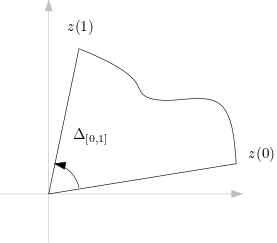
\includegraphics[scale=0.8]{deltaarg.png}
    \caption{Приращение аргумента вдоль кривой}
		\label{fig:14.1}
\end{figure}\\
\theorem (логарифмическое свойство)
Пусть $z(t) \in C^1[0;1]$, $\forall t \in [0,1] z(t) \neq 0$. Пусть $z(t) =
z_1(t)z_2(t)$, $z_k(t) \in C^1[0,1]$. Тогда
\begin{equation}\label{(14.8)}
    \Delta_{[0,1]}\argt z = \Delta_{[0,1]}\argt z_1 + \Delta_{[0,1]}\argt z_2
\end{equation}
\pr
Из \eqref{(14.7)} имеем:
\begin{align*}
  & \Delta_{[0,1]} \argt z(t) = \Img \int_{0}^{1}\frac{\left( z_1(\tau)z_2(\tau) \right)'}{z_1(\tau)z_2(\tau)}d \tau =\Img \int_{0}^{1}\frac{z_1'z_2+z_1z_2'}{z_1z_2}d \tau = \Img \int_{0}^{1}\frac{z_1'}{z_1}d \tau + \Img \int_{0}^{1}\frac{z_2'}{z_2}d \tau = \\
  & = \Delta_{[0,1]} \argt z_1(t) \Delta_{[0,1]} \argt z_2(t) 
\end{align*}
\Def
Пусть $\gamma$~--- кривая в $\CC$, заданная параметризацией $z=z(t)$, $t \in
[0;1]$, $z \in C^1[0;1]$, $0 \not \in \gamma$. Тогда \textbf{приращением
  аргумента $z$ вдоль кривой $\gamma$} называется
\begin{equation}\label{(14.9)}
    \Delta_{\gamma}\argt z = \Delta_{[0;1]}\argt z = \Img \int_{0}^1 \frac{z'(\tau)}{z(\tau)}d \tau
\end{equation}
Определение корректно, т.~к. \eqref{(14.9)} равносильно
\begin{equation}\label{(14.10)}
    \Delta_{\gamma}\argt z = \Img \int_{\gamma} \frac{dz}{z}
\end{equation}
    \begin{flushright}
    \textit{Лекция 11 (от 12.10)}
\end{flushright}
\section{$\S 15.$ Регулярные ветви многозначных функций $\{\sqrt{z}\}$ и $\Ln z$.}

    \begin{flushright}
    \textit{Лекция 12 (от 13.10)}
\end{flushright}
\corollary
Пусть $G$ односвязна, $0 \not \in G$. Тогда для регулярной $h_k \in \Ln z$
справедлива формула Ньютона-Лейбница
\begin{equation}\label{(15.14)}
    h_k(z) = h_k(a) + \int_{\gamma_{az}}\frac{d\zeta}{\zeta}
\end{equation}
где $a \in G$, $\gamma_{az} \subseteq G$.
\pr
\begin{align*}
  & h_k(z) = h_0(z) + 2i \pi k
\end{align*}
\begin{align*}
  & h_0(z) = \ln \left| z \right| + i \left( \psi_0 + \Delta_{\gamma_{az}}\argt z \right)
\end{align*}
\begin{align*}
  & \Real \int_{\gamma_{az}} \frac{d\zeta}{\zeta} = \ln \left| z \right| - \ln \left| a \right|
\end{align*}
Действительно, пусть $z(t) = \gamma_{az}$, тогда
\begin{align*}
  & \Real \int_{\gamma_{az}} \frac{d\zeta}{\zeta} = \Real \int_0^1 \frac{xx'+yy'}{x^2+y^2} d \tau = \Real \int_0^1 \frac{d \sqrt{x^2+y^2}}{\sqrt{x^2+y^2}} = \ln \left| z(1) \right| - \ln \left| z(0) \right| = \ln \left| z \right| - \ln \left| a \right|
\end{align*}
\begin{align*}
  & h_k(z) = \ln \left| z \right| - \ln \left| a \right| + \ln\left| a \right| + i \left( \psi_0 + 2 \pi k \right) + i \Delta_{\gamma_{az}}\argt z = h_k(a) + \int_{\gamma_{az}}\frac{d\zeta}{\zeta}
\end{align*}
\section{$\S 16$. Регулярные ветви $\{\sqrt[n]{f(z)}\}$ и $\ln f(z)$.}
\sug
$G$~--- область, $f$ регулярна на $G$, $\forall z \in G \ f(z) \neq 0$.
\begin{equation}\label{(16.1)}
    \left\{ \sqrt[n]{f(z)} \right\} = \sqrt[n]{\left| f(z) \right|} \exp \left( \frac{i}{n}\Arg f(z) \right)
\end{equation}
\begin{equation}\label{(16.2)}
    \Ln f(z) = \ln \left| f(z) \right| +i \Arg f(z)
\end{equation}
\begin{equation}\label{(16.3)}
    \Arg f(z) = \left\{ \argt f(z) + 2 \pi k \mid k \in \ZZ \right\}
\end{equation}
\Def
Пусть $\gamma$~--- непрерывная кривая в $G$, $f$ удовлетворяет предположению
$1$. Пусть $z(t)$~--- параметризация $\gamma$, $t \in [0;1]$. Пусть $\Gamma =
f(\gamma): \ w = f(z(t)), \ t \in [0;1]$. Тогда \textbf{приращением аргумента
  $f(z)$ вдоль кривой $\gamma$} называется
\begin{equation}\label{(16.4)}
    \Delta_{\gamma}\argt f(z) = \Delta_\Gamma\argt w = \Delta_{[0;1]}\argt f(z(t))
\end{equation}
\lemma
Пусть $f$, $f_1$, $f_2$ удовлетворяют предположению $1$ в области $G$. Тогда
\begin{enumerate}
    \item для любой непрерывной $\gamma \subseteq G$ выполняется логарифмическое
    свойство:
    \begin{equation}\label{(16.5)}
        \Delta_{\gamma}\argt (f_1f_2) = \Delta_\gamma\argt f_1 + \Delta_{\gamma}\argt f_2
    \end{equation}
    \item если $\gamma \subseteq G$ разбита точкой $A \in \gamma$ на части
    $\gamma_1$, $\gamma_2$, то
    \begin{equation}\label{(16.6)}
        \Delta_{\gamma}\argt f = \Delta_{\gamma_1}\argt f + \Delta_{\gamma_2}\argt f
    \end{equation}
    \item если $\gamma$~--- кусочно гладкая кривая в $G$, то
    \begin{equation}\label{(16.7)}
        \Delta_{\gamma}\argt f(z) = \Img \int_\Gamma \frac{dw}{w} = \Img \int_{\gamma} \frac{f'(\zeta)}{f(\zeta)}d\zeta
    \end{equation}
\end{enumerate}
\pr
Утверждения леммы очевидны из определения приращения аргумента функции.
\lemma
Пусть $G$ односвязна, $\os{\circ}{\gamma} \subseteq G$ замкнута и непрерывна.
Пусть $f$ удовлетворяет предположению $1$. Тогда
\begin{equation}\label{(16.8)}
    \Delta_{\os{\circ}{\gamma}}\argt f(z) = 0
\end{equation}
\pr
Пусть $\os {\circ}{\gamma} \subseteq G$ гладкая и замкнутая, параметризованная
$z(t)$.
\\
$\forall z_0 \in \os{\circ}{\gamma}$ существует непрерывная деформация $z(t,
\alpha)$ такая, что $z(t,a) = z(t)$, $z(t,b) = z_0$. По теореме $3$ $\S 14$
$I(\alpha) = const$, а значит,
\begin{align*}
  \Delta_{[0;1]}\argt f(z) = \Delta_{[0;1]}\argt f(z_0) = 0
\end{align*}
\lemma
Пусть $f$ удовлетворяет предположению $1$ в области $G$. Если в области $G$
сществуют регулярные ветви $h_0(z)$ или $g_0(z)$~--- регулярные ветви $\Ln f(z)$
или $\left\{ \sqrt[n]{f(z)} \right\}$, то все их непрерывные ветви регулярны и
удовлетворяют соотношениям:
\begin{equation}\label{(16.9)}
    h_k(z) = h_0(z) + 2i \pi k, \ k \in \ZZ
\end{equation}
\begin{equation}\label{(16.10)}
    g_k(z) = g_0(z) \exp\left( \frac{i}{n} 2 \pi k\right), \ k \in \{0, \dots, n-1\}
\end{equation}
\pr
Доказательство полностью аналогично доказательству леммы $15.1$.
\lemma
Пусть $f$ удовлетворяет предположению $1$ в $G$. Если в $G$ существует
регулярная ветвь $h(z)$ многозначной функции $\Ln z$, то $\forall a,b \in G$
\begin{equation}\label{(16.11)}
    h(b) = h(a) + \ln \left| \frac{f(b)}{f(a)} \right| + i \Delta_{\gamma_{ab}}\argt f(z)
\end{equation}
\pr
\begin{align*}
  & h(z) = \ln \left| f(z) \right| + i \Img h(z)
\end{align*}
В силу регулярности $h$ $\Img h$ будет гармонической функцией от $x, y$. Значит,
\begin{align*}
  & \varphi(z) = \Img h(z) \in \Arg f(z)
\end{align*}
Пусть $a \in G$, $\psi_0 \in \Arg f(a)$, $h(a) = \ln \left| f(a) \right| + i
\psi_0$. Пусть $\gamma_{az}$~--- гладкая кривая с параметризацией $z(t)$, $t \in
[0;1]$, $\varphi(z(t))$~--- гладкая ветвь $\Arg f(z(t))$.
\begin{align*}
  & \Delta_{\gamma_{az}}\argt f(z) = \varphi(z(1))-\varphi(z(0)) = \Img h(z) - \Img h(a)
\end{align*}
\begin{align*}
  & h(b) = \ln \left| f(b) \right| + i \Img h(b)
\end{align*}
\begin{align*}
  & h(a) = \ln \left| f(a) \right| + i \Img h(a)
\end{align*}
\begin{align*}
  & h(b) - h(a) = \ln \left| \frac{f(b)}{f(a)} \right| + i \left( \Img h(b) - \Img h(a) \right)
\end{align*}
Отсюда следует \eqref{(16.11)}.
\theorem
Пусть $f$ удовлетворяет предположению $1$ в $G$. Тогда у  $\Ln f(z)$ существуют
регулярные ветви в $G$ тогда и только тогда, когда выполняется \eqref{(16.8)}
для любой замкнутой $\os{\circ}{\gamma}\subseteq G$.
\pr
Докажем в обе стороны.
\begin{itemize}
    \item Необходимость.
    \\
    Если есть регулярные ветви $h(z) \in \Ln z$  $G$, то из \eqref{(16.11)} при
    $a = b$ получаем \eqref{(16.8)}.
    \item Достаточность.
    \\
    Пусть выполнено \eqref{(16.8)}. Фиксируем $a \in G$, $h(a) \in \Ln f(a)$.
    Рассмотрим
    \begin{equation}\label{(16.12)}
        h(z) = h(a) + \ln \left| \frac{f(z)}{f(a)} \right| + i \Delta_{\gamma_{az}}\argt f(z)
    \end{equation}
    В действительности приращение аргумента может зависеть от $\gamma$, поэтому
    корректнее расссматривать это как $h(\gamma_{az})$.
    \\
    По \eqref{(16.8)}
    \begin{align*}
      & \Delta_{\gamma_{az}}\argt f(z) = \Delta_{\tilde{\gamma}_{az}} f(z)
    \end{align*}
    \begin{align*}
      & \os{\circ}{\gamma} = \gamma_{az}+\tilde{gamma}^{-1}_{az}
    \end{align*}
    Значит, $h(z)$~--- функция лишь точки $z$.
    \begin{equation}\label{(16.13)}
        \exists \psi_0 \in \Arg f(a): \ h(a) = \ln \left| f(a) \right| + i \psi_0
    \end{equation}
    Из \eqref{(16.12)} следует, что
    \begin{align*}
      & h(z) = \ln \left| f(z) \right| + i \left( \psi_0 + \Delta_{\gamma_{az}}\argt f(z) \right) \in \Ln f(z)
    \end{align*}
    \begin{align*}
      & \Real \int_{\gamma_{az}}\frac{f'(\zeta)}{f(\zeta)}d\zeta = \ln \left| f(z) \right| - \ln \left| f(a) \right|
    \end{align*}
    \begin{align*}
      & \Delta_{\gamma_{az}}\argt f(z) = \Img \int_{\gamma_{az}}\frac{f'(\zeta)}{f(\zeta)}d\zeta
    \end{align*}
    Отсюда следует, что
    \begin{align*}
      & h(z) = \ln \left| f(a) \right| + \ln \left| f(z) \right| - \ln \left| f(a) \right| + i \Delta_{\gamma_{az}} \argt f(z) + i \psi_0 = \ln \left| f(a) \right| + \int_{\gamma_{az}}\frac{f'(\zeta)}{f(\zeta)}d \zeta
    \end{align*}
    Функция
    \begin{align*}
      & \varphi(z) = \int_{\gamma_{az}}\frac{f'(\zeta)}{f(\zeta)}d\zeta
    \end{align*}
    регулярна по теореме $3$ $\S 6$, а значит, и $h(z)$ регулярна.
\end{itemize}
\lemma
Пусть $f$ удовлетворяет предположению $1$ в $G$, $n \in \NN$, $n \geq 2$. Если в
$G$ существует регулярная ветвь $g(z)$ многозначной функции $\left\{
    \sqrt[n]{f(z)} \right\}$, то $\forall a, b \in G$
\begin{equation}\label{(16.14)}
    g(b) = g(a) \sqrt[n]{\left| \frac{f(b)}{f(a)} \right|}\exp \left( \frac{1}{n}\Delta_{\gamma_{ab}}\argt f(z) \right)
\end{equation}
\pr Доказательство разбиваем на два этама.
\begin{enumerate}
    \item $G$ односвязна.
    \\
    По лемме $2$ $\forall \os{\circ}{\gamma} \subseteq G$ выполняется
    \eqref{(16.8)}:
    \begin{align*}
      & \exists h(z) = h(a) + \ln \left|\frac{f(z)}{f(a)}\right|+ i\left(\Delta_{\gamma_{az}}\argt f(z)\right) \in \Ln f(z)
    \end{align*}
    регулярные ветви.
    \begin{align*}
      & g_0(z) = \exp \left(\frac{i}{n} h(z)\right)
    \end{align*}
    \begin{align*}
      & \exists \psi_0 \in \Arg f(a): \ h(z) = \ln \left| f(z) \right| + i \left( \psi_0 + \Delta_{\gamma_{az}}\argt f(z) \right)
    \end{align*}
    Тогда
    \begin{align*}
      & g_0(z) = \sqrt[n]{\left| f(z) \right|}\exp \left( \frac{i}{n} \left( \psi_0 + \Delta_{\gamma_{az}}\argt f(z) \right) \right)\in \left\{ \sqrt[n]{f(z)} \right\}
    \end{align*}
    регулярная ветвь.
    \\
    По лемме $3$ $\exists k \in \left\{ 0, \dots, n-1 \right\}: \ g(z) = g_0(z)$.
    Отсюда следует \eqref{(16.14)}.
    \item $G$~--- область.
    \begin{align*}
      &\forall a, b \in G, \ \forall \gamma_{ab} \subseteq G
    \end{align*}
    можем выбрать такие $a=z_0, z_1, \dots, z_{K-1}, z_K = b \in \gamma_{ab}$,
    что $\left| z_k - z_{k-1} \right|< l_k$, где $l_k$~--- расстояние до
    границы.
    \begin{align*}
      & \exists \left\{ B_\varepsilon(z_k) \right\}_{k=0}^K \subseteq G: \ z_{k+1} \in B_{\varepsilon}(z_k)
    \end{align*}
    Каждый из $B_{\varepsilon}(z_k)$ односвязен, поэтому выполняется
    \eqref{(16.14)}:
    \begin{align*}
      & \forall k \in \left\{ 0, \dots, K-1 \right\} \ \frac{g(z_{k+1})}{g(z_k)} = \sqrt[n]{\frac{f(z_{k+1})}{f(z_k)}} \exp \left( \frac{i}{n} \Delta_{\gamma_{z_kz_{k+1}}}\argt f(z) \right)
    \end{align*}
    Перемножая по всем $k$, получаем
    \begin{align*}
      & \frac{g(b)}{g(a)} = \sqrt[n]{\left| \frac{f(b)}{f(a)} \right|}\exp \left( \frac{i}{n} \sum_{k=0}^{K-1} \Delta_{\gamma_{z_kz_{k+1}}} \argt f(z) \right) = \sqrt[n]{\frac{\left| f(b) \right|}{\left| f(a) \right|}}\exp \left( \frac{i}{n}\Delta_{\gamma_{ab}}\argt f(z) \right)
    \end{align*}
    Это ни что иное, как \eqref{(16.14)}.
\end{enumerate}\theorem
Пусть $f$ удовлетворяет условиям предположения $1$ в $G$. Тогда существуют
регуляртые ветви $\left\{ \sqrt[n]{f(z)} \right\}$тогда и только тогда, когда
\begin{equation}\label{(16.15)}
    \forall \os{\circ}{\gamma} \subseteq G \exists k(\os{\circ}{\gamma}) \in \ZZ: \ \Delta_{\os{\circ}{\gamma}}\argt f(z) = 2\pi n k(\os{\circ}{\gamma}))
\end{equation}
    \begin{flushright}
    \textit{Лекция 13 (от 19.10)}
\end{flushright}
\pr
Из леммы $5$ очевидно следует необходимость (возьмем $a = b$).
\\
Докажем достаточность. Пусть $a \in G$, $z \in G$, $\gamma_{az}\in G$, $g(a) \in
\left\{ \sqrt[n]{f(z)} \right\}$. Тогда выполняется
\begin{equation}\label{(16.16)}
    g(z) = g(a) \sqrt[n]{\left| \frac{f(b)}{f(a)} \right|}\exp \left( \frac{i}{n} \Delta_{\gamma_{az}}\arg f(z) \right)
\end{equation}
Докажем регулярность такой ветви.
\\
Для замкнутых кривых экспонента примет значение $1$, а значит, $g(z)$ зависит
только от точки $z$. Очевидно, $\forall z \in G \ g(z)\in \left\{ \sqrt[n]{f(z)}
\right\}$. Докажем ее регулярность.
\\
Фиксируем произвольную $z_1 \in G$; тогда $\exists B_\varepsilon(z_1) \subseteq G$
такой, что
\begin{equation}\label{(16.17)}
    \forall z \in B_\varepsilon(z_1) \ g(z) = g(z_1) \sqrt[n]{\left| \frac{f(z)}{f(z_1)} \right|}\exp \left( \frac{i}{n} \Delta_{\gamma_{z_1z}}\argt f(z) \right)
\end{equation}
$B_{\varepsilon}(z_1)$ односвязна, значит, по лемме $2$
$\Delta_{\os{\circ}{\gamma}}\argt f(z) = 0$ для любой замкнутой
$\os{\circ}{\gamma} \subseteq B_\varepsilon(z_1)$. Но
\begin{align*}
  & g(z) = \exp \left( \frac{i}{n} h(z) \right)
\end{align*}
\begin{align*}
  & h(z) = \ln \left| f(z) \right| + i \left(\psi_0 + \Delta_{\gamma_{z_1z}}\argt f(z)\right), \ \psi_0 \in \Arg f(z_1)
\end{align*}
\begin{equation}\label{(16.18)}
    g(z_1) = \sqrt[n]{\abs{f(z_1)}} \exp\left( \frac{i}{n}\psi_0 \right)
\end{equation}
В $B_\varepsilon(z_1)$ есть регулярная ветвь $\Ln f(z)$, причем $h(z)$~--- та
самая ветвь, значит, $g(z)$ регулярна в $B_\varepsilon(z_1)$.
\\
В силу произвольности выбора $z_1$ показали регулярность во всей $G$.
\corollary
Если $h(z)$, $g(z)$~--- регулярные ветви $\Ln f(z)$ и $\left\{ \sqrt[n]{f(z)}
\right\}$ соответственно в $G$, то
\begin{equation}\label{(16.19)}
    h'(z) = \frac{f'(z)}{f(z)}
\end{equation}
\begin{equation}\label{(16.20)}
    g'(z) = \frac{f'(z)}{n\left( g(z) \right)^{n-1}}
\end{equation}
\pr
\begin{align*}
  & e^{h(z)} \equiv f(z) \rightarrow h'(z)e^{h(z)} \equiv f'(z) \Rightarrow h'(z) \equiv \frac{f'(z)}{f(z)}
\end{align*}
\begin{align*}
  & (g(z))^n \equiv f(z) \Rightarrow n(g(z))^{n-1}g'(z) \equiv f'(z) \Rightarrow g'(z) = \frac{f'(z)}{n\left( g(z) \right)^{n-1}}
\end{align*}
\section{$\S 17.$ Примеры вычисления регулярных ветвей.}
\Example
\begin{align*}
  & \left\{ \sqrt[4]{z^3(z+1)} \right\}, \ G = \CC \setminus[-1;0]
\end{align*}
Если ветвь существует, то
\begin{align*}
  & g_1(2) = i \sqrt[4]{24}
\end{align*}
При этих условиях найти $g_1(i)$, $g'_1(i)$.
\nonum
Заметим: $f(z) = z^3(z+1)$, $n=4$. Видим, что в $G$ $f(z) \neq 0$.
\\
$\forall \os{\circ}{\gamma} \subseteq G$~--- замкнутой~--- рассмотрим
$\Delta_{\os{\circ}{\gamma}}\argt f(z)$.
\begin{align*}
  & \Delta_{\os{\circ}{\gamma}}\argt f(z) = \Delta_{\os{\circ}{\gamma}}\argt z^3(z+1) = 3 \Delta_{\os{\circ}{\gamma}}\argt z + \Delta_{\os{\circ}{\gamma}}\argt (z-1)
\end{align*}
\begin{figure}[h!]
		\centering
		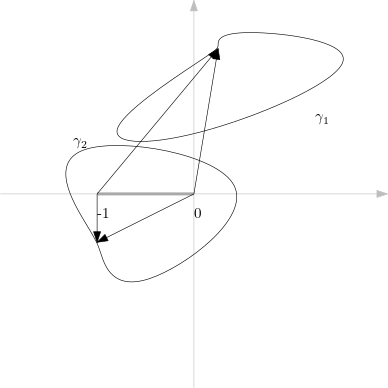
\includegraphics[scale=0.5]{Ex1.png}
		\label{fig:17.1}
\end{figure}
На кривых вида $\gamma_1$ (не опоясывающих разрез) приращение обоих аргументов
равно нулю (а значит, и суммарное), а на кривых вида $\gamma_2$ приращение
аргумента составит $8 \pi$. Оба случая удовлетворяют условию существования
регулярных ветвей.
\\
Докажем строго. Пусть $\os{\circ}{\gamma} = z(t)$, $t \in [0;1]$, $z(0) = z(1) =
z_0 \in \gamma$, $z(t, \alpha) = z(t) - \alpha$, $\alpha \in [-1;0]$. $\forall
(t, \alpha) \ z(t, \alpha) \neq 0$, $\forall \alpha \ z(1, \alpha) = z(0,
\alpha) = z_0 - \alpha$. Значит, по теореме $3$ $\S 14$ $I(\alpha) =
\Delta_{[0;1]}\argt z(t, \alpha) = const$, т.~е.
\begin{align*}
  & \Delta_{[0;1]} \argt z(t) = \Delta_{[0;1]} \argt(z(t) + 1) = \Delta_{\os{\circ}{\gamma}}z = \Delta_{\os{\circ}{\gamma}}(z+1) = 2 \pi k(\os{\circ}{\gamma})
\end{align*}
\begin{align*}
  & \Delta_{\ogamma} \argt f(z) = 4 \Delta_{\ogamma} \argt z = 8 \pi
\end{align*}
Желаемое условие выполняется.
\\
Значит,
\begin{align*}
  & g_1(z) = g_1(2) \sqrt[4]{\frac{\left| z^3(z+1) \right|}{24}} \exp \left( \frac{i}{4}\left( \Delta_{\gamma{2z}}\argt f(z) \right) \right)
\end{align*}
\begin{align*}
  & g_1(i) = g_1(2) \sqrt[4]{\frac{\left| i^3(i+1) \right|}{24}} \exp \left( \frac{i}{4}\left( \Delta_{\gamma_{2,i}}\argt f(z) \right) \right) = 2^{\frac{1}{8}}i\exp \left( \frac{i}{4} \left( 3\Delta_{\gamma_{2,i}}\argt z + \Delta_{\gamma_{2,i}} \argt (z+1) \right) \right) = \\
  & = 2^{\frac{1}{8}}i\exp \left( \frac{i}{4} \left( 3\frac{\pi}{2} + \frac{\pi}{4} \right) \right) = 2^{\frac{1}{8}}i\exp \left( \frac{7i\pi}{16} \right) =  2^{\frac{1}{8}}e^{\frac{15i\pi}{16}}
\end{align*}
\begin{align*}
  & g_1'(z) = \frac{4z^3+3z^2}{4g_1^3(z)}
\end{align*}
\begin{align*}
  & g_1'(i) = \frac{-4i -3}{4\cdot 2^{\frac{3}{8}}e^{\frac{45i\pi}{16}}} = -(4i+3)2^{-\frac{19}{8}}e^{-\frac{13i\pi}{16}}
\end{align*}
\Example
\begin{align*}
  & \Ln (1-z^2), \ G = \CC \setminus (-\infty; 1]
\end{align*}
Если ветвь существует, то
\begin{align*}
  & \Img h\left( \frac{i}{5} \right) = 0
\end{align*}
При этих условиях найти разложение $h$ в ряд Тейлора по степеням $(z+i)$,
область, где $h(z) = S(z)$~--- сумма своего ряда Тейлора, его радиус сходимости
$R$ и $S\left( \dst \frac{i}{5} \right)$.
\nonum
$G$ односвязна. Заметим: $f(z) = 1-z^2 \neq 0$ в $G$.
\\
$\forall \gamma \subseteq G$ рассмотрим $\Delta_{\gamma}\argt f(z)$.
\begin{align*}
  & h(z) = \ln \left| z \right| + i \Img h(z)
\end{align*}
\begin{align*}
  & h\left( \frac{i}{5} \right) = \ln \frac{26}{25}
\end{align*}
\begin{figure}[h!]
		\centering
		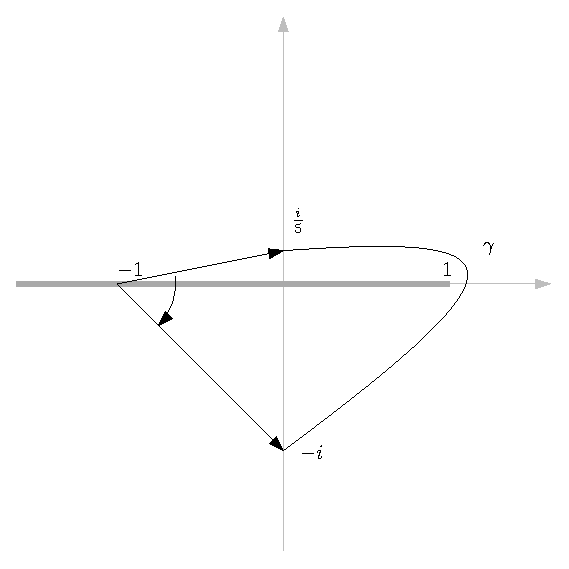
\includegraphics[scale=0.75]{Ex1.eps}
		\label{fig:17.2}
\end{figure}
\begin{align*}
  & h(-i) = \ln \frac{26}{25} + \ln \left| \frac{2}{\frac{26}{25}} \right|+ i\left( \Delta_{\gamma_{\frac{i}{5}, -i}}\argt (z+1) + \Delta_{\gamma_{\frac{i}{5}, -i}}\argt (z-1) + \Delta_{\gamma_{\frac{i}{5}, -i}}\argt (-1) \right) = \ln 2 - 2 i \pi
\end{align*}
Положим $\zeta = z+i$, $h(z) = h(\zeta - i) = \tilde{h}(\zeta)$. Тогда
$\tilde{h}(0) = h(-i) = \ln 2 - 2 i \pi$. Хотим разложить это в ряд.
\begin{align*}
  & \tilde{h}(\zeta) \in \Ln (1-(\zeta - i)^2) = \Ln(2+2i\zeta - \zeta^2) = \Ln \left(2\left( 1 - \frac{\zeta}{1-i} \right)\left( 1 - \frac{\zeta}{1+i} \right) \right) = \Ln 2 + \\
  & \Ln \left( 1 - \frac{\zeta}{1-i} \right) + \Ln \left( 1 - \frac{\zeta}{1+i} \right)
\end{align*}
Из теоремы об обратной функции
\begin{align*}
  & h^*_k(z) \in \Ln (1+z), \ \left| z \right| < 1 \Rightarrow h^*_k(z) = 2 i \pi k + \sum_{n=1}^\infty \frac{(-1)^{n+1}}{n} z^n, \ \left| z \right| < 1
\end{align*}
Рассмотрим
\begin{align*}
  & h_+(\zeta) \in \Ln \left( 1 - \frac{\zeta}{1+i} \right), \ \left| \zeta \right| < \sqrt{2}, \ h_+(0) = 0 \Rightarrow h_+(\zeta) = - \sum_{n=1}^\infty \frac{\zeta^n}{n(1+i)^n}, \ \left| \zeta \right| < \sqrt{2}
\end{align*}
\begin{align*}
  & h_-(\zeta) \in \Ln \left( 1 - \frac{\zeta}{1-i} \right), \ \left| \zeta \right| < \sqrt{2}, \ h_-(0) = 0 \Rightarrow h_-(\zeta) = - \sum_{n=1}^\infty \frac{\zeta^n}{n(1-i)^n}, \ \left| \zeta \right| < \sqrt{2}
\end{align*}
Заметим, что $\sqrt{2}$~--- максимальный радиус, т.~к. выходим на особую точку.
Видим:
\begin{align*}
  & \tilde{h}(\zeta) - h_+(\zeta) - h_-(\zeta) = \ln 2 + 2 i \pi k(\zeta)
\end{align*}
В правой части функция непрерывная, в левой ступенчатая, значит, $k = const$.
Найдем ее:
\begin{align*}
  &  \tilde{h}(0) - h_+(0) - h_-(0) = \ln 2 + 2 i \pi k = \ln 2 - 2 i \pi
\end{align*}
Значит, $k = -1$.
\\
Значит,
\begin{align*}
  & \tilde{h}(\zeta) = - \sum_{n=1}^\infty \frac{\zeta^n}{n(1+i)^n} - \sum_{n=1}^\infty \frac{\zeta^n}{n(1-i)^n} + \ln 2 - 2 i \pi
\end{align*}
\begin{align*}
  & h(z) = - \sum_{n=1}^\infty \frac{1}{n}\left( \frac{1}{(1+i)^n}+ \frac{1}{(1-i)^n}\right)(z-i)^n + \ln 2 - 2 i \pi, \ \left| z-i \right|< \sqrt{2}
\end{align*}
Видим, что $S(z)$ регулярна на $\left| z-i \right|< \sqrt{2}$; $S(z)$ и $h(z)$
есть регулярные ветви логарифма. Но также можем заметить, что часть разреза
лежит внутри круга сходимости. Тогда
\begin{align*}
  & \forall x \in (-1;1) \ h(x + i0) = h(x-i0) + i\Delta_{x+i0, x-i0}\argt h(z) = h(x-i0) + 2 i \pi \neq h(x-i0)
\end{align*}
Значит, внутри круга при положительной мнимой части $h(z) = S(z) + 2 i \pi$, а
при отрицательной мнимой части $h(z) = S(z)$.
\\
Значит,
\begin{align*}
  & S\left( \frac{i}{5} \right) = \ln \frac{25}{26} - 2 i \pi
\end{align*}
\begin{align*}
  & S'\left( \frac{i}{5} \right) = \left. \frac{-2z}{(1-z^2)} \right|_{z=\frac{i}{5}} = \frac{-2i\cdot 25}{5\cdot 26} = -\frac{5i}{13}
\end{align*}
\Def
Пусть $a, b \in \CC$, $a \neq 0$. Тогда
\begin{equation}\label{(17.1)}
    \left\{ a^b \right\} = \exp\left( b \Ln a\right)
\end{equation}
\Exse
Если $b = n$ или $b = \dst \frac{1}{n}$, $n\in \NN$, то \eqref{(17.1)} описывает
$a^n$ или $\left\{ \sqrt[n]{a} \right\}$ соответственно.
\Example
Разложить в ряд Тейлора регулярные ветви функции
\begin{align*}
  & \left\{ (1+z)^b \right\}, \ \left| z \right|<1
\end{align*}
\nonum
По определению,
\begin{align*}
  & (1+z)^b = \exp \left( b \Ln (1+z) \right)
\end{align*}
В силу существования регулярных ветвей у логарифма в этом круге ($h_k(0) = 2 i
\pi k$, $h_k$~--- регулярные ветви), то есть и регулярные ветви данной функции
будут существовать и иметь вид $w_k(z) = \exp \left( b h_k(z) \right)$.
\Exse
Доказать, что любая регулярная ветвь этой функции имеет такой вид.
\\
Вычислим производные $w_k$.
\begin{align*}
  & w_k(0) = e^{2bi\pi k}
\end{align*}
\begin{align*}
  & w_k'(z) = w_k(z) \frac{b}{1+z} \Rightarrow w_k'(0) = be^{2bi\pi k}
\end{align*}
\begin{align*}
  & w_k''(z) = w_k(z) \frac{b(b-1)}{(1+z)^2} \Rightarrow w_k''(0) = b(b-1)e^{2bi\pi k}
\end{align*}
\begin{align*}
  & w_k^{(n)}(z) = w_k(z) \frac{b(b-1)\dots(b-n+1)}{(1+z)^n} \Rightarrow w_k^{(n)}(0) = b(b-1)\dots(b-n+1)e^{2bi\pi k}
\end{align*}
\begin{align*}
  & w_k(z) = w_k(0)\sum_{n=0}^\infty C_b^nz^n
\end{align*}
\Example
Разложить в ряд Тейлора функцию
\begin{align*}
  & g \in \left\{ \sqrt[3]{1-z^2} \right\}, \ B_1(0), \ g(0) = \exp \left( \frac{2 i \pi}{3} \right)
\end{align*}
\nonum
По аналогии с предыдущим примером,
\begin{align*}
  & g(z) = \exp \left( \frac{2 i \pi}{3}\sum_{n=1}^\infty C_{\frac{1}{3}}^n(-1)^n z^{2n} \right)
\end{align*}
\Example
Разложить в $\os{\circ}{B}_1(\infty)$ в ряд Лорана регулярные ветви функции
\begin{align*}
  & \sets{\sqrt[4]{z^3(z+1)}}
\end{align*}
\nonum
\begin{align*}
  & \os{\circ}{B}_1(\infty) = \left\{ z \mid \left| z \right| > 1\right\}\subseteq \CC \setminus [-1;1]
\end{align*}
По аналогии с примером $1$
\begin{align*}
  & g_k(z) = \sqrt[4]{24}\exp \left( \frac{i\pi k}{2} \right)
\end{align*}
При $x > 2$, $x \in \RR$
\begin{align*}
  & g_0(x) = \sqrt[4]{x^3(x+1)} = x \sqrt[4]{1+\frac{1}{x}} = x \sum_{n=1}^\infty C_{\frac{1}{4}}^n\left( \frac{1}{x} \right)^n = S(x)
\end{align*}
\begin{align*}
  & \forall x \in \RR \cap (2; \infty) \ g_0(x) = S(x)
\end{align*}
Обе функции $S(z)$ и $g_0(z)$ регулярны, и по теореме единственности $g_0(z) =
S(z)$, а значит, искомый ряд Лорана будет иметь вид
\begin{align*}
  & z \sum_{n=1}^\infty C_{\frac{1}{4}}^n\left( \frac{1}{z} \right)^n
\end{align*}

    \begin{flushright}
    \textit{Лекция 14 (от 20.10)}
\end{flushright}
\section{$\S 18.$ Вычисление интегралов от регулярных ветвей.}
\Example
Вычислить при помощи теории вычетов интеграл
\begin{align*}
  & I = \int_0^2 \frac{\sqrt[4]{x^3(2-x)}}{(1+x)^2} dx
\end{align*}
\nonum
$g(z) = \sqrt[4]{z^3(2-z)}$ дает многозначную функцию. Отыщем регулярные ветви;
рассмотрим область, где ветви существуют. Функция $f(z) = z^3(2-z)$ должна быть
в области регулярной и не равной нулю.
\\
Рассмотрим $\CC \setminus [0;2]$. В такой области этот корень имеет регулярную
ветвь.
\\
Отыщем ветвь, что нам нужна. Построим ее так, чтобы $g(1+i0) = 1$; тогда
$\forall x \in [0;2] \ g(x+i0) = \sqrt[4]{x^3(2-x)}$. В этом случае
\begin{align*}
  & g(x-i0) = g(1+i0)\exp\left( \frac{i}{4}\left( 3\Delta_{\gamma_{1+i0,x}}\argt z + \Delta_{\gamma_{1+i0,x}}\argt (2-z) \right) \right) = \exp\left( \frac{-i\pi}{2}\right)
\end{align*}
\begin{figure}[h!]
		\centering
		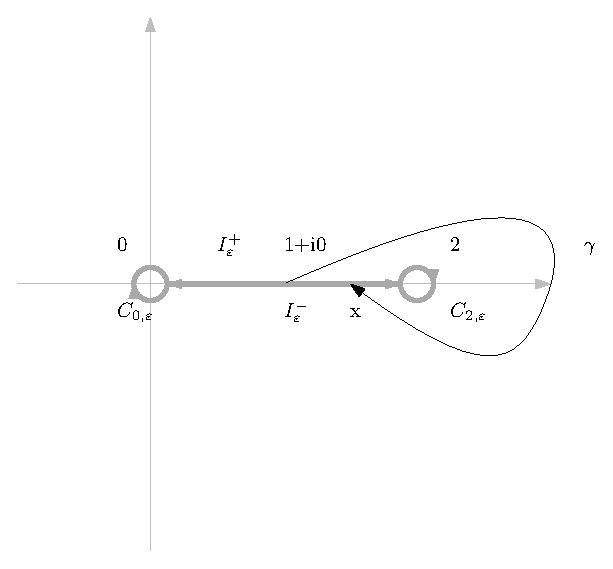
\includegraphics[scale=0.75]{Par18.eps}
		\label{fig:18.1}
\end{figure}
Рассмотрим
\begin{align*}
  & \gamma_\varepsilon = I_\varepsilon^+\cup C_{2, \varepsilon} \cup I_\varepsilon^-\cup C_{0, \varepsilon}
\end{align*}
и
\begin{align*}
  & F(z) = \frac{\sqrt[4]{z^3(2-z)}}{(1+z)^2} = \frac{g(z)}{(1+z)^2}
\end{align*}
и вычислим
\begin{align*}
  & I_\varepsilon = \int_{\gamma_\varepsilon}F(z) dz = 2 i \pi \left( \us{-1}{\res} F(z) + \us{\infty}{\res} F(z) \right)
\end{align*}
Видим, что $-1$~--- полюс $2$ порядка, а $\infty$~--- УОТ.
\begin{align*}
  & \us{-1}{\res} F(z) = \lim_{z \to -1}((z+1)^2F(z))' = \lim_{z \to -1}g'(z) = g'(-1) = \frac{f'(z)}{4g^3(z)}\mid_{z = -1} = \frac{-4(-1)^3+6(-1)^2}{4\left( \sqrt[4]{3}\exp\left( \frac{3i\pi}{4} \right)\right)^3} = \\
  & = \frac{5}{2\sqrt[4]{27}}\exp\left( \frac{-i\pi}{4} \right)
\end{align*}
Рассмотрим $x \in (2; \infty)$; тогда
\begin{align*}
  & g(x) = \sqrt[4]{x^3(2-x)}\exp\left( \frac{-i\pi}{4} \right) = x\sqrt[4]{1-\frac{2}{x}}\exp \left( \frac{-i\pi}{4} \right) = x\exp\left( \frac{-i\pi}{4} \right)\sum_{n=0}^\infty C_{\frac{1}{4}}^n\left( -\frac{2}{x} \right)^n
\end{align*}
Две регулярные функции ($g(x)$ и сумма) совпадают на $(2; \infty)$, а значит, по
теореме единственности
\begin{align*}
  & g(z) = z\exp\left( \frac{-i\pi}{4} \right)\sum_{n=0}^\infty C_{\frac{1}{4}}^n\left( -\frac{2}{z} \right)^n, \ \left| z \right|> 2
\end{align*}
\begin{align*}
  & F(z) = \frac{z}{(z+1)^2}h(z), \ h(z) = \exp\left( \frac{-i\pi}{4} \right)\sum_{n=0}^\infty C_{\frac{1}{4}}^n\left( -\frac{2}{z} \right)^n
\end{align*}
Заметим, что
\begin{align*}
  & \frac{z}{(1+z)^2} = \frac{1}{z(1+\frac{1}{z})^2} = \frac{1}{z} \left( 1-\frac{2}{z} +\frac{3}{z^2} + \dots \right)
\end{align*}
При перемножении двух рядов получим
\begin{align*}
  & \us{\infty}{\res}F(z) = -\exp\left( \frac{-i\pi}{4} \right)
\end{align*}
и интеграл
\begin{align*}
  & I_\varepsilon = 2 i \pi \left( \frac{5}{2\sqrt[4]{27}} - 1 \right)\exp\left( \frac{-i\pi}{4} \right)
\end{align*}
не зависит от $\varepsilon$. Заметим, что
\begin{align*}
  & I_\varepsilon = \int_{I_\varepsilon^+}F(z) + \int_{C_{2, \varepsilon}}F(z) + \int_{I_\varepsilon^-}F(z) + \int_{C_{0, \varepsilon}}F(z)
\end{align*}
Причем
\begin{align*}
  & \int_{I_\varepsilon^+}F(z) = \int_{\varepsilon}^{2-\varepsilon}\frac{\sqrt[4]{x^3(2-x)}}{(x+1)^2}dx
\end{align*}
\begin{align*}
  & \int_{I_\varepsilon^-}F(z) = \int_{2-\varepsilon}^{\varepsilon}\frac{g(x-i0)}{(x+1)^2}dx = -\int_{\varepsilon}^{2-\varepsilon}\frac{\sqrt[4]{x^3(2-x)}\exp\left( \frac{3i\pi}{2} \right)}{(x+1)^2}dx = -\exp\left( \frac{3i\pi}{2}\right) \int_{I_\varepsilon^+}F(z)
\end{align*}
Учтя $z = \varepsilon e^{i \varphi}$,
\begin{align*}
  & \left|  \int_{C_{0, \varepsilon}}F(z) \right| \leq \int_{0}^{2 \pi}\frac{\sqrt[4]{\varepsilon^3(2+\varepsilon)}\varepsilon}{(1-\varepsilon)^2}d\varphi \leq A\varepsilon^{\frac{7}{3}} \us{\varepsilon \to 0}{\to} 0
\end{align*}
Учтя $z = 2 + \varepsilon e^{i \varphi}$,
\begin{align*}
  & \left|  \int_{C_{2, \varepsilon}}F(z) \right| \leq \int_{0}^{2 \pi}\frac{\sqrt[4]{(2+\varepsilon)^3\varepsilon}\varepsilon}{(3-\varepsilon)^2}d\varphi \leq B\varepsilon^{\frac{4}{3}} \us{\varepsilon \to 0}{\to} 0
\end{align*}
Значит,
\begin{align*}
  & 2 i \pi \left( \frac{5}{2\sqrt[4]{27}} - 1 \right)\exp\left( \frac{-i\pi}{4} \right) = I_\varepsilon \us{\varepsilon \to 0}{\to} \int_{I_\varepsilon^+}F(z) + \int_{I_\varepsilon^-}F(z) = \left( 1 -\exp\left( \frac{3i\pi}{2}\right) \right) \int_{I_\varepsilon^+}F(z) \us{\varepsilon \to 0}{\to} \\
  & \us{\varepsilon \to 0}{\to} \left( 1 -\exp\left( \frac{3i\pi}{2}\right) \right) I
\end{align*}
Значит,
\begin{align*}
  & I = \frac{2 i \pi \left( \dst \frac{5}{2\sqrt[4]{27}} - 1 \right)\exp\left( \dst\frac{-i\pi}{4} \right)}{\left( 1 -\exp\left( \dst \frac{3i\pi}{2}\right) \right)}= \pi \sqrt{2}\left( \dst \frac{5}{2\sqrt[4]{27}} - 1 \right)
\end{align*}
\section{$\S 19.$ Целые и мероморфные функции.}
\Def
Функция $f$ называется \textbf{целой}, если она регулярна на $\CC$.
\\
Можем представить такую функцию в виде
\begin{equation}\label{(19.1)}
    \forall z \in \CC \ f(z) = \sum_{n=0}^\infty c_nz^n, \ c_n = \frac{1}{2i\pi}\int_{\gamma_r}\frac{f(\zeta)}{\zeta^{n+1}} d \zeta
\end{equation}
\theorem
Пусть $f:G \mapsto \CC$ целая, $\exists A > 0, \ R > 0, \ m \in \NN_0$ такие,
что $\forall z: \left| z \right| > R \hookrightarrow \left| f(z) \right| \leq
A\left| z \right|^m$. Тогда $f(z)$~--- многочлен степени $\leq m$.
\pr
Воспользуемся оценкой $c_n$.
\begin{align*}
  & \forall r > R \ \left|c_n \right| \leq \frac{1}{2\pi}\int_{\left| \zeta \right| = r} \frac{\left| f(\zeta) \right|}{\left| \zeta \right|^{n+1}}\left| d\zeta \right|\leq \frac{1}{2\pi}\frac{Ar^m}{r^{n+1}}r\cdot 2 \pi = Ar^{m-n}
\end{align*}
Значит, $\forall n > m \ c_n = 0$.
\corollary (теорема Лиувилля)
Если $f$ целая, $\exists R > 0, \ A > 0$: $\left| f(z) \right|< A$ при $\left| z
\right| < R$, то $f \equiv const$.
\theorem (Основная теорема алгебры)
Всякий многочлен $P_n(z) = z^n + C_{n-1}z^{n-1}+\dots+c_0$ имеет в $\CC$ хотя бы
один корень.
\pr
предположим, $\forall z \in \CC \ P_n(z) \neq 0$. Тогда $\varphi(z) = \dst
\frac{1}{P_n(z)}$ целая. Но, как легко видеть,
\begin{align*}
  & \lim_{z \to \infty}P_n(z) = \infty \Rightarrow \lim_{z \to \infty} \varphi(z) = 0 \Rightarrow \exists R > 0: \ \forall z: \ \left| z \right| > R \hookrightarrow \left| \varphi(z) \right| < 1
\end{align*}
Значит, по теореме Лиувилля $\varphi(z) = const$, тогда и $P_n(z) = const$.
Противоречие.
\\
Значит, можем заметить, что для целой функции $f$ единственная особая точка~---
это $\infty$.
\begin{itemize}
    \item $\infty$~--- УОТ, тогда $f = const$.
    \item $\infty$~--- полюс порядка $m$, тогда $f = P_m$.
    \item $\infty$~--- СОТ.
\end{itemize}
\Def
Целая функция, у которой $\infty$ есть СОТ, назвается \textbf{целой
  трансцендентной}.
\theorem (Сохоцкого)
Пусть $f$~--- целая трансцендентная функция, тогда
\begin{align*}
  & \forall A \in \CCC \ \exists z_n \to \infty: \ \lim_{n \to \infty}f(z_n) = A
\end{align*}
\pr
Рассмотрим два случая.
\begin{itemize}
    \item $A = \infty$
    \\
    $f$ неограничена в окрестности $\infty$ (т.~к. иначе она бы имела конечный
    предел), т.~е.
    \begin{align*}
      & \forall n \in \NN \exists z_n \in \CC: \left| f(z_n) \right|> n, \ \left| z_n \right| > n
    \end{align*}
    Итак, $\left\{ z_n \right\}$ и есть та самая последовательность.
    \item $A \in \CC$
    \\
    Пусть, от противного,
    \begin{align*}
      & \exists \delta_0 > 0, \ \varepsilon_0 > 0: \ \forall z: \ \left| z \right| \geq \delta_0 \ \left| f(z) - A \right| \geq \varepsilon_0
    \end{align*}
    Пусть $\varphi(z) = \dst \frac{1}{f(z) - A}$, $z \in B_{\delta_0}(\infty)$.
    На этом множестве
    \begin{align*}
      & \left| \varphi(z) \right| \leq \frac{1}{\varepsilon_0}
    \end{align*}
    Значит, эта функция на этом множестве регулярна и ограничена, а значит, для
    нее $\infty$~--- УОТ, т.~е.
    \begin{align*}
      & \exists \lim_{z \to \infty}\varphi(z) = B
    \end{align*}
    Значит, $\infty$~--- полюс либо УОТ для $f(z)$, противоречие.
\end{itemize}
\theorem (общая теорема Сохоцкого)
Пусть $f: \os{\circ}{B}_r(a) \mapsto \CC$ регулярна, $a$~--- СОТ $f$. Тогда
\begin{align*}
  & \forall A \in \CCC \ \exists z_n \to a, \ \lim_{n \to \infty} f(z_n) = A
\end{align*}
\Exse
доказать общую теорему Сохоцкого.
\theorem (Пикара)
Пусть $f$~--- целая трансцедентная функция, тогда $\forall a \in \CC$, за
исключением, быть может, одного, $\exists R > 0$: в $\os{\circ}{B}_R(\infty)$
существует бесконечное число решений уравнения $f(z) = A$, т.~е.
\begin{align*}
  & \exists z_n \to \infty: \ \forall n \in \NN \ f(z_n) = A
\end{align*}
\Example
$e^z = A$ имеет счетное число решений в любой окрестности при $A \neq 0$, но ни
одного решения при $A = 0$.
\Exse
Пусть $f$~--- целая функция и
\begin{align*}
  & \exists A > 0, R > 0, \ m \in \NN_0: \ \forall z: \ \left| z \right| > R \ \left| f(z) \right| \geq A \left| z \right|^m
\end{align*}
Доказать, что $f$~--- многочлен степени $\leq m$.
\Def
Функция $f$ называется мероморфной, если $\forall R > 0$ в круге $B_R(0)$ она
регулярна за исключением, быть может, конечного числа полюсов.
\Example
\begin{align*}
  & f(z) = \frac{P_n(z)}{Q_m(z)}
\end{align*}
Конечное число полюсов на всей $\CC$.
\Example
\begin{align*}
  & f(z) = \ctg z
\end{align*}
Счетное число полюсов на $\CC$.
\Example
\begin{align*}
  & f(z) = \frac{z}{e^z-1}
\end{align*}
Счетное число полюсов на $\CC$.
    \begin{flushright}
    \textit{Лекция 15 (от 26.10)}
\end{flushright}
\section{$\S 20.$ Принцип аргумента. Теорема Руше.}

    \begin{flushright}
    \textit{Лекция 16 (от 27.10)}
\end{flushright}
\theorem (Руше)
Пусть $G$~--- односвязная область, $\ogamma$~--- замкнутая положительно
ориентированная кусочно гладкая кривая в этой области. Пусть $f,g: G \mapsto
\CC$ регулярны, и
\begin{equation}\label{(20.3)}
    \forall z \in \ogamma \ \left| f(z) \right| > \left| g(z) \right|
\end{equation}
Тогда $f(z)$ и $h(z) = f(z)+g(z)$ имеют внутри $\ogamma$ одинаковое число нулей
с учетом их порядка.
\pr
\begin{align*}
  & \forall z \in \ogamma \ \left| f(z) \right| > \left| g(z) \right| \Rightarrow \forall z \in \ogamma \ f(z) \neq 0
\end{align*}
\begin{align*}
  & \forall z \in \ogamma \ \left| h(z) \right|\geq \left| f(z) \right| - \left| g(z) \right| > 0 \Rightarrow \forall z \in \ogamma h(z) \neq 0
\end{align*}
\begin{align*}
  & \Delta_{\ogamma}\argt h(z) = \Delta_{\ogamma} \argt \left( f(z)\left( 1+\frac{g(z)}{f(z)} \right) \right) = \Delta_{\ogamma}\argt f(z) +\Delta_{\ogamma}\argt \left( 1+\frac{g(z)}{f(z)} \right)
\end{align*}
\begin{align*}
  & \ogamma: w = 1 + \frac{g(z)}{f(z)} \Rightarrow \left| w-1 \right| = \left| \frac{g(z)}{f(z)} \right| < 1
\end{align*}
Пусть $\Gamma = w(\ogamma)$; $0 \not \in B_1(1)$ и эта область односвязна,
значит, по лемме $2$ $\S 14$
\begin{align*}
  & \Delta_{\ogamma}\argt \left( 1+\frac{g(z)}{f(z)} \right) = 0
\end{align*}
и тогда
\begin{align*}
  & N_h = \frac{1}{2\pi}\Delta_{\ogamma}\argt h(z) = \frac{1}{2\pi}\Delta_{\ogamma}\argt f(z) = N_f
\end{align*}
\theorem (Гаусса)
Многочлен
\begin{align*}
  & P_n(z) = c_0+zc_1+z^2c_2+\dots+z^nc_n
\end{align*}
имеет в $\CC$ ровно $n$ корней с учетом их порядка.
\pr
Рассмотрим $f(z) = z^n$, $g(z) = P_n(z) - f(z)$. Как известно,
\begin{align*}
  & \left| \frac{g(z)}{f(z)} \right| \us{z \to \infty}{\to} 0 \Rightarrow \exists R_0 > 0: \ \forall R \geq R_0 \ \forall z \in \gamma_R \left| f(z) \right| > \left| g(z) \right|
\end{align*}
Значит, по теореме Руше функция $P_n(z)$ имеет столько же нулей, сколько и $f(z)
= z^n$, на $B_R(0)$, с учетом порядка, т.~е. ровно $n$ штук.
\Example
Функция Жуковского
\begin{align*}
  & w = \frac{1}{2}\left( z+\frac{1}{z} \right)
\end{align*}
У функции $\pm i$~--- нули, $0$~--- полюс первого порядка.
\\
Рассматривая $R>1$, получим
\begin{align*}
  & \Delta_{\gamma_R}\argt w(z) = 2 \pi (N-P) = 2\pi
\end{align*}
\begin{align*}
  & \Delta_{\gamma_{\frac{1}{R}}}\argt w(z) = 2 \pi (N-P) = -2\pi
\end{align*}
\section{$\S 21.$ Геометрические принципы.}
\lemma (об открытости)
Пусть $f$ регулярна в $G$, $z_0 \in G$, $w_0 = f(z_0)$.
\\
Пусть при $n \geq 2$
\begin{equation}\label{(20.1)}
    f'(z_0) = \dots = f^{(n-1)}(z_0) = 0, \ f^{(n)}(z_0) \neq 0
\end{equation}
Тогда $\exists B_\delta(z_0)$ и $B_\varepsilon(w_0)$, такие, что $\forall w_1
\in B_{\varepsilon}(w_0)$ уравнение $f(z) = w_1$ имеет в круге $B_\delta(z_0)$
ровно $n$ решений.
\pr
Заметим, что $f(z) \neq const$, $f'(z) \neq const$. Тогда по теореме
единственности нули функции $f(z)-w_0$ и $f'(z)$ изолированы, поэтому
\begin{align*}
& \exists \delta > 0: \ \forall z \in \ol{\os{\circ}B_\delta(z_0)} \ f(z)-w_0 \neq 0, \ f'(z) \neq 0
\end{align*}
Пусть $\gamma = \left\{ z: \left| z-z_0 \right| = \delta \right\}$ положительно
ориентирована, и $\forall z \in \gamma \ f(z)\neq w_0$. Положим $0 < \varepsilon
= \inf \left\{ w_0 - f(z) \mid z \in \gamma \right\}$, $\Gamma = f(\gamma)$.
заметим, что $\Gamma$ замкнута и $w_0 \not \in \Gamma$.
\\
Тогда
\begin{align*}
& \forall w_1 \in \os{\circ}{B}_\varepsilon(w_0), \ \forall z \in \gamma \ \left| w_1-w_0 \right| < \varepsilon \leq \left| w_0 - f(z) \right|
\end{align*}
Пусть $F(z) = w_0 - f(z)$, $G(z) = w_1-w_0$. Тогда $H(z) = F(z)+G(z) =
w_1-f(z)$; значит, по теореме Руше (в силу $\left| F(z) \right|> \left| G(z)
\right|$) функции $w_0 - f(z)$ и $w_1-f(z)$ имеют одинаковое число нулей внутри
$\gamma$. 
\\
Заметим, что $f(z) = w_0$ имеет единственный нуль~--- $z_0$~--- порядка $n$.
Значит, с учетом порядка $f(z) = w_1$ имеет $n$ решений.
\\
Но 
\begin{align*}
& \forall z \in B_\delta(z_0) \ f'(z) = (f(z)-w_1)' \neq 0
\end{align*}
Значит, все нули будут иметь первый порядок, соответственно, их ровно $n$ штук.
\corollary
Пусть $f$ регулярна в $G \subseteq \CC$. Тогда $\forall z_0 \in G$ условие
$f'(z_0) = 0$ необходимо и достаточно для однолистности $f$ <<в малом>>~--- в
некоторой достаточно малой окрестности $z_0$, но не во всей $G$.
\Example
$w=e^z$ удовлетворяет условиям следствия, но не однолистна во всей комплексной
плоскости.
\theorem (принцип сохранения области)
Пусть $f$ регулярна в области $G$, причем $f(z) \neq const$. Тогда $f(G)$~---
также область.
\pr
Докажем открытость.
\begin{align*}
& \forall z_0 \in G \ w_0 = f(z_0) \in G^* = f(G)
\end{align*}
Поскольку $G$~--- область, 
\begin{align*}
& \exists \delta_1: \ B_{\delta_1}(z_0) \subseteq G
\end{align*}
и по лемме $20.1$
\begin{align*}
& \exists \delta \in (0; \delta_1], \ \exists \varepsilon > 0: \ \forall w_1 \in B_\varepsilon (w_0) \ \exists z_1 \in B_\delta(z_0): \ f(z_1) = w_1; \ f(B_\delta(z_0)) \supseteq B_\varepsilon(w_0)
\end{align*}
Значит, $B_\varepsilon(w_0)\in G^*$, т.~е. $w_0$~--- внутренняя точка $G^*$.
\\
Докажем связность.
\begin{align*}
  & \forall w_1, w_2 \in G^* \ \exists z_1,z_2 \in G: \ \exists \gamma_{z_1z_2} \subseteq G, \ \Gamma_{w_1w_2} = f(\gamma_{z_1z_2}) \subseteq G^*
\end{align*}
\theorem (принцип максимума модуля регулярной функции)
Пусть $f: G \mapsto \CC$ регулярна в ограниченной области $G$, непрерывна на ее
замыкании и непостоянна. Тогда
\begin{align*}
  & \max_{z \in \ol{G}} \left| f(z) \right| = \max_{z \in \partial G} \left| f(z) \right|
\end{align*}
\pr
Путь, от противного,
\begin{align*}
  & \exists z_0 \in G: \ \left| f(z_0) \right| = \max_{z \in \ol{G}}\left| f(z) \right|
\end{align*}
Пусть $w_0 = f(z_0)$. По теореме $20.1$
\begin{align*}
  & \exists \varepsilon > 0, \ B_\varepsilon(w_0) \subseteq f(G) = G^*
\end{align*}
\begin{align*}
  & w_1 \in B_\varepsilon(w_0): \left| w_1 \right| > \left| w_0 \right|; \ w_1 = w_0\left( 1+\frac{\varepsilon}{2\left| w_0 \right|} \right)
\end{align*}
\begin{align*}
  & \exists z_1 \in G: \ f(z_1) = w_1; \ \left| f(z_1) \right| > \left| f(z_0) \right|
\end{align*}
Противоречие.
\corollary (принцип минимума модуля регулярной функции)
Пусть $f: G \mapsto \CC$ регулярна в ограниченной области $G$, непрерывна на ее
замыкании и непостоянна. Тогда
\begin{align*}
  & \min_{z \in \ol{G}} \left| f(z) \right| = \min_{z \in \partial G} \left| f(z) \right|
\end{align*}
\Note
Для случая неограниченной $G$ вместо $\min$ и $\max$ используется $\inf$ и
$\sup$.
\lemma (Шварца)
Пусть $f: B_1(0) \mapsto \CC$ регулярна, $\forall z \in B_1(0) \ \left| f(z)
\right| \leq 1$, $f(0) = 0$. Тогда выполняется
\begin{equation}\label{(21.2)}
    \forall z \in B_1(0) \ \left| f(z) \right| \leq z
\end{equation}
Если в \eqref{(21.2)} достигается равенство при $z_0 \neq 0$, то
\begin{align*}
  & \exists \alpha \in \RR: \ \forall z \in \ol{B_1(0)} \ f(z) = e^{i\alpha}z
\end{align*}
\pr
$f(0) = 0$, а значит, существует регулярная в $B_1(0)$ функция $g(z)$: $f(z) =
zg(z)$. Функция $g(z) = \dst \frac{f(z)}{z}$, но при этом регулярна также и в
нуле.
\\
Рассмотрим произвольное $r \in (0;1)$ и $z: \ \left| z \right|<r$. По теореме
$2$
\begin{align*}
  & \left| g(z) \right| \leq \max \left\{ \left| \frac{f(\zeta)}{\zeta} \right| : \left| \zeta \right| =r \right\} \leq \frac{1}{r}
\end{align*}
Пусть $z_0 \in B_1(0)$; $\forall f \in (\left| z_0 \right|, 1)$ $\left| g(z_0)
\right| \leq \dst \frac{1}{r}$, а значит, $\left| g(z_0) \right|\leq 0$, и
$\forall z \in B_1(0) \ \left| f(z) \right|\leq \left| z \right|$.
\\
Пусть равенство в \eqref{(20.2)} достигается в некоторой точке $z_1$ (т.~е.
$\left| g(z) \right| = 1$). Поскольку точка лежит внутри области, то либо
возникает противоречие с принципом максимума, либо $g(z) = const = e^{i
  \alpha}$.
\theorem (принцип максимума и минимума гармонической функции)
Пусть $u: G \mapsto \CC$ гармоническая на $G \subseteq \RR^2$ и непостоянная,
непрерывная на $\ol{G}$. Тогда $\sup$ и $\inf$ функции $u$ на $G$ и $\ol{G}$
совпадают.
\pr
Допустим, $\exists z_0 = (x_0, y_0)\in G$, на которой $u$ достигает максимума.
Тогда $\exists \varepsilon > 0: \ B_\varepsilon(z_0)\subseteq G$; по теореме $2$
$\S 4$ сущствует регулярная $f$ в $B_\varepsilon(z_0)$ такая, что $\Real f(z) =
u(z)$.
\\
$w_0 = f(z_0)$; по теореме $21.1$ $f(B_\varepsilon(z_0))$~--- область, т.~е.
$\exists r > 0$: $B_r(w_0) \subseteq f(B_{\varepsilon}(z_0))$. Пусть $w_1 \in
B_r(w_0)$, $\Real w_1 > \Real w_0$.
\\
Значит,
\begin{align*}
  \exists z_1 \in B_\varepsilon(z_0): \ w_1 = f(z_1), \ \Real f(z_1) > \Real f(z_0) \Rightarrow u(z_1)>u(z_0)
\end{align*}
Противоречие.
\\
В силу $\inf u(z) = - \sup(-u(z))$, гармоничности $-u(z)$ и выполнимости
принципа максимума выполняется и принцип миминума.
\theorem (о среднем для гармонической функции)
Пусть $u: B_R(z) \mapsto \RR$ гармоническая и непрерывная на замыкании
этого круга, непостоянная. Тогда
\begin{equation}\label{(21.3)}
    u(a) = \frac{1}{2\pi}\int_0^{2\pi}u(a+Re^{i\varphi})d\varphi
\end{equation}
\pr
По теореме $2$ $\S 14$ существует $f: B_R(a) \mapsto \CC$~--- регулярная, причем
$\forall z \in B_R(a) \ \Real f(z) = u(z)$, $0<\rho < R$, $\gamma_\rho =
\left\{ z: \left| z-a \right| = \rho\right\}$.
\begin{align*}
  & f(a) = \frac{1}{2 i \pi}\int_{\gamma_\rho}\frac{f(\zeta)}{\zeta - a}d\zeta = \frac{1}{2i\pi}\int_0^{2\pi}\frac{f(a+\rho e^{i\varphi})}{\rho e^{i\varphi}} i \rho e^{i\varphi} d \varphi = \frac{1}{2\pi}\int_0^{2\pi}f(a+\rho e^{i\varphi})d \varphi
\end{align*}
\begin{align*}
  & \Real f(a) = u(a) = \frac{1}{2\pi}\int_0^{2\pi}\Real f(a+\rho e^{i\varphi})d \varphi = \frac{1}{2\pi}\int_0^{2\pi}u (a+\rho e^{i\varphi})d \varphi
\end{align*}
Устремляя $\rho \to R$, получаем \eqref{(21.3)}.

    \begin{flushright}
    \textit{Лекция 17 (от 02.11)}
\end{flushright}
\section{$\S 22.$ Конформные отображения в $\overline{\CC}$.}
\section{$\S 23.$ Дробно-линейные функции.}

    \begin{flushright}
    \textit{Лекция 18 (от 03.11)}
\end{flushright}
\theorem
При ДЛО пара симметричных точек относительно окружности или прямой $\gamma$
переходит в пару симметричных точек относительно образа $\gamma$ (окружности или
прямой).
\lemma
Точки $z$ и $z^*$ симметричны относительно окружности или прямой $\gamma$ тогда
и только тогда, когда любая окружность или прямая $\Gamma$: $z, z^* \in \Gamma$
перпендикулярна $\gamma$.
\pr (леммы)
\\
Рассмотрим случай, когда $\gamma$~--- окружность. 
\begin{itemize}
    \item Необходимость.
    \\
    Пусть $\Gamma$~--- также окружность, поскольку случай с прямой очевиден.
    \begin{figure}[h!]
        \centering
        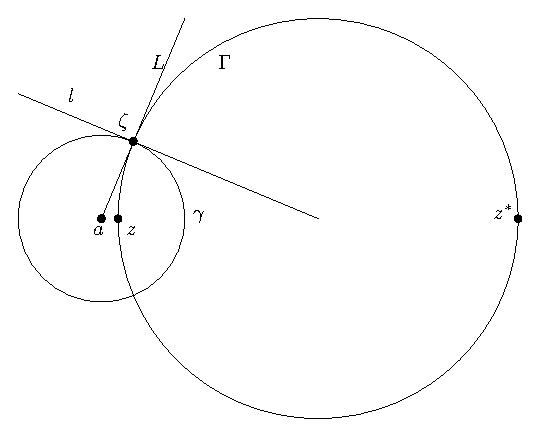
\includegraphics[scale=0.75]{neob.eps}
        \label{fig:23.1}
    \end{figure}
    Пусть $L$~--- касательная к $\Gamma$ из $A$, $\zeta \in L \cap \Gamma$.
    Тогда
    \begin{align*}
      & \left| a - \zeta \right| = \left| a-z \right|\cdot \left| a-z^* \right| = R^2
    \end{align*}
    а значит, $\zeta \in \gamma$. Пусть $l$~--- касательная к $\Gamma$ в точке
    $\zeta$, $l \perp [a;\zeta] \Rightarrow l \perp L$.
    \item Достаточность.
    \begin{itemize}
        \item $\Gamma$~--- прямая, тогда $a \in \Gamma$, и значит, $z$ и $z^*$
        принадлежат одной полупрямой, исходящей из центра (иначе прямые $l$ и
        $L$ не перпендикулярны).
        \item $\Gamma$~--- окружность, тогда пусть $\zeta \in \Gamma \cap
        \gamma$, тогда
        \begin{align*}
          & \left| a - \zeta \right|^2 = \left| a-z \right|\cdot \left| a-z^* \right| = R^2
        \end{align*}
    \end{itemize}
\end{itemize}
\pr (теоремы)
$z$, $z^*$ симметричны относительно $\gamma$ (пусть окружности). Пусть $f$~---
ДЛО \eqref{(23.1)}, \eqref{(23.2)}. Пусть $w = f(z)$, $w^* = f(z^*)$, нужно
доказать, что они симметричны относительно $\tilde{\gamma} = f(\gamma)$.
\\
Рассмотрим $w$, $w^*$. Пусть $\tilde{\Gamma}$~--- любая окружность или прямая,
такая, что $w, w^* \in \tilde{\Gamma}$. Значит, поругоому свойству существует
окружность или прямая$\Gamma$: $\tilde{\Gamma} = f(\Gamma)$. По свойству
однолистности $z, z^* \in \Gamma$. Значит, по лемме $1$ $\gamma \perp \Gamma$.
Тогда, посвойству сохранения углов, $\tilde{\Gamma} \perp \tilde{\gamma}$. По
лемме $1$ тогда $w$ и $w^*$ симметричны относительно $\tilde{\Gamma}$.
\theorem
Множество ДЛО образует группу отображений относительно операции суперпозиции.
\pr
~
\begin{itemize}
    \item Очевидно, существует единичный элемент~--- тождественное отображение.
    \item У каждого ДЛО существует и единственно обратное ДЛО (см. теорему $1$).
    \item Суперпозиция ДЛО есть ДЛО. Действительно, пусть
    \begin{align*}
      & \zeta = \frac{a_1z+b_1}{c_1z+d_1}, \ w = \frac{a_2z+b_2}{c_2z+d_2}, \ a_1d_1 - c_1d_1 \neq 0, \ a_2d_2 - b_2c_2 \neq 0
    \end{align*}
    Положим
    \begin{align*}
      & z = \frac{z_1}{z_2}, \ \zeta = \frac{\zeta_1}{\zeta_2}, \ w = \frac{w_1}{w_2}
    \end{align*}
    Тогда
    \begin{align*}
      & \left( \begin{matrix}
              \zeta_1 \\
              \zeta_2
          \end{matrix} \right) = \left( \begin{matrix}
              a_1 & b_1 \\
              c_1 & d_1
          \end{matrix} \right) \cdot \left( \begin{matrix}
              z_1 \\
              z_2
          \end{matrix} \right), \ \left( \begin{matrix}
              w_1 \\
              w_2
          \end{matrix} \right) = \left( \begin{matrix}
              a_2 & b_2 \\
              c_2 & d_2
          \end{matrix} \right) \cdot \left( \begin{matrix}
              \zeta_1 \\
              \zeta_2
          \end{matrix} \right)
    \end{align*}
    \begin{align*}
      & \left( \begin{matrix}
              w_1 \\
              w_2
          \end{matrix} \right) = \left( \begin{matrix}
              a_2 & b_2 \\
              c_2 & d_2
          \end{matrix} \right) \cdot \left( \begin{matrix}
              a_1 & b_1 \\
              c_1 & d_1
          \end{matrix} \right) \cdot \left( \begin{matrix}
              z_1 \\
              z_2
          \end{matrix} \right)
    \end{align*}
    Получили невырожденное ДЛО.
\end{itemize}
\Example
Отобразить с помощью ДЛО области (см. рис.)
\begin{figure}[h!]
    \begin{minipage}[c]{0.45\textwidth}
        \centering
        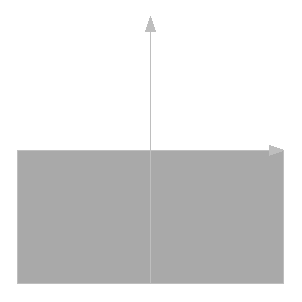
\includegraphics[scale=0.5]{half_plane.eps}
    \end{minipage}
    \begin{minipage}[c]{0.1\textwidth}
        \centering
        \LARGE{$\mapsto$}
    \end{minipage}
    \begin{minipage}[c]{0.45\textwidth}
        \centering
        
\includegraphics[scale=0.5]{round.eps}
    \end{minipage}
    \label{fig:23.2}
    \caption{$\Img z > 0 \mapsto \left| z \right| > 1$}
\end{figure}
\nonum
Возьмем любую $z_0: \ \Img z_0 > 0$. Пусть $z_0 \mapsto 0$, тогда $\bar{z_0}
\mapsto \infty$.
\\
Тогда
\begin{align*}
    & w = A\frac{z-z_0}{z-\ol{z_0}}
\end{align*}
Отыщем теперь $A$. Граница отображается на границу. Возьмем $x \in \RR$, она
должна лежать на единичную окружность. Тогда
\begin{align*}
    & 1 = \abs{w} = \abs{A\frac{x-z_0}{x+\ol{z_0}}} = \left| A \right| = e^{i\alpha}
\end{align*}
Итак,
\begin{equation}\label{(23.6)}
    w = e^{i \alpha}\frac{z-z_0}{z-\ol{z_0}}
\end{equation}
\Example
Отобразить с помощью ДЛО области (см. рис.).
\\
\begin{figure}[h!]
    \begin{minipage}[c]{0.45\textwidth}
        \centering
        
\includegraphics[scale=0.5]{round.eps}
    \end{minipage}
    \begin{minipage}[c]{0.1\textwidth}
        \centering
        \LARGE{$\mapsto$}
    \end{minipage}
    \begin{minipage}[c]{0.45\textwidth}
        \centering
        
\includegraphics[scale=0.5]{round.eps}
    \end{minipage}
    \label{fig:23.3}
    \caption{$\left| z \right| > 1 \mapsto \left| z \right| > 1$}
\end{figure}
\nonum
Возьмем произвольную $z_0$ и отобразим ее в ноль; тогда симметричная $z_0^* =
\dst \frac{1}{\ol{z_0}}$ перейдет в $\infty$.
\\
Тогда
\begin{align*}
    & w = A\frac{z-z_0}{z-\dst \frac{1}{\ol{z_0}}} = \tilde{A}\frac{z-z_0}{1 - z\ol{z_0}}
\end{align*}
Граница перейдет в границу, а значит,
\begin{align*}
    & 1 = \abs{w} = \abs{\tilde{A}\frac{e^{i \varphi}-z_0}{1 - e^{i \varphi}\ol{z_0}}} = \abs{\tilde{A}\frac{e^{i \varphi}-z_0}{e^{-i \varphi}-\ol{z_0}}} = \abs{\tilde{A}}
\end{align*}
Итак,
\begin{equation}\label{(23.7)}
    w = e^{i \alpha}\frac{z-z_0}{1 - z\ol{z_0}}
\end{equation}
\Example
Отобразить с помощью ДЛО три различные точки $z_1, z_2, z_3$ в три точки $w_1,
w_2,w_3$.
\nonum
Заметим, что условиям удовлетворяет отображение вида
\begin{equation}\label{(23.8)}
    h(z) = \frac{z-z_1}{z-z_2} \cdot \frac{z_3-z_2}{z_3-z_1} = \frac{w-w_1}{w-w_2} \cdot \frac{w_3-w_2}{w_3-w_1} = g(w)
\end{equation}
\begin{align*}
  & w = f(z) = g^{-1}(h(z))
\end{align*}
Существование получено. Докажем единственность.
\\
Пусть для начала $f(z_k) = z_k$, тогда
\begin{align*}
  & \frac{az_k + b}{cz_k+d} = z_k
\end{align*}
\begin{align*}
  & cz^2_k + (d-a)z_k - b = 0
\end{align*}
Значит, поскольку квадратное уравнение имеет три решения, все его коэффициенты
равны нулю. Значит, $f(z) = z$.
\\
Пусть существуют $f_1(z)$, $f_2(z)$, причем $f_1(z_k) = f_2(z_k) = w_k$; тогда
$z_k = f_1^{-1}(f_2(z_k))$, тогда по групповому свойству $f_1^{-1}(z) =
f_2^{-1}(z)$, а значит, $f_1(z) = f_2(z)$.
\Example
Отобразить с помощью ДЛО области (см. рис.).
\\
\begin{figure}[h!]
    \begin{minipage}[c]{0.45\textwidth}
        \centering
        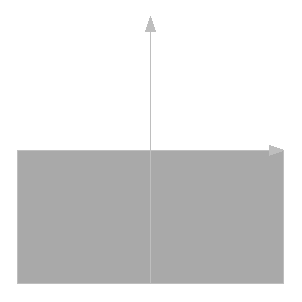
\includegraphics[scale=0.5]{half_plane.eps}
    \end{minipage}
    \begin{minipage}[c]{0.1\textwidth}
        \centering
        \LARGE{$\mapsto$}
    \end{minipage}
    \begin{minipage}[c]{0.45\textwidth}
        \centering
        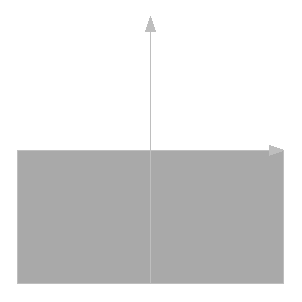
\includegraphics[scale=0.5]{half_plane.eps}
    \end{minipage}
    \label{fig:23.4}
    \caption{$\Img z > 0 \mapsto \Img z > 0$}
\end{figure}
\nonum
Пусть $x_1, x_2, x_3 \in \RR$, $x_1 < x_2 < x_3$, $u_1, u_2, u_3 \in \RR$, $u_1
< u_2 < u_3$, построим отображение $f(x_) = u_k$. по примеру $3$ такое
отображение существует и единственно, границу оно переводит в границу. Из
свойства сохранения углов следует сохранение ориентации границы. Рассматривая
\eqref{(23.8)}, получаем все действительные  коэффициенты, т.~е. $a, b, c, d \in
\RR$, тогда $\forall x \in \RR \ \argm w'(x) = 0 \Rightarrow w'(x) > 0$, т.~е.
\begin{align*}
  & w'(x) = \frac{ad-cb}{(cx+d)^2} > 0 \Leftrightarrow ad-cb > 0
\end{align*}
Итак, необходимо и достаточно, чтобы все коэффициенты ДЛО были действительны,
причем $ad-cb > 0$.
\section{$\S 24.$ Конформные отображения элементарными функциями. Теорема Римама.}
Рассмотрим функции, обладающие локальной однолистностью.
\begin{center}
    \textbf{Степенная функция}
\end{center}
Фиксируем $t > 0$, рассмотрим область $G = \CC \setminus [0;+\infty)$. Пусть
\begin{align*}
  & w = \left| z \right|^t \exp(it \argt z), \ \argt z \in (0, 2 \pi)
\end{align*}
Функция регулярна при любом $t$. Действительно,
\begin{align*}
  & h(z) = \ln \left| z \right| + i \argt_0 z
\end{align*}
регулярна на этой области, а
\begin{align*}
  & w = \exp(t h(z))
\end{align*}
регулярна в этой области, как суперпозиция регулярных функций.
\\
Исследуем теперь однолистность. Рассмотрим
\begin{align*}
  & G_{0,\varphi_0} = \left\{ z \mid \left| z \right| > 0, \ \argt z \in (0; \varphi_0)\right\}
\end{align*}
\begin{align*}
  & l_{\varphi} = \left\{ z \mid z = r e^{i \varphi}, \ r > 0, \ \varphi \in (0, \varphi_0)\right\}
\end{align*}
Тогда
\begin{align*}
  & w(l_\varphi) = \left\{ w \mid w = \rho e^{i t \varphi}, \ \rho > 0 \right\}
\end{align*}
Тогда условие однолистности:
\begin{align*}
  & \begin{cases}
      0 < \varphi_0 < 2 \pi \\
      0 < t \varphi_0 < 2 \pi
  \end{cases}
\end{align*}
Значит, функция конформна на этой области.
\Example
$t = 2$, $w = z^2$.
\\
Условие однолистности: $\varphi_0 \in (0; \pi)$.
\\
\begin{figure}[h!]
    \begin{minipage}[c]{0.45\textwidth}
        \centering
        
\includegraphics[scale=0.5]{half_round.eps}
    \end{minipage}
    \begin{minipage}[c]{0.1\textwidth}
        \centering
        \LARGE{$\mapsto$}
    \end{minipage}
    \begin{minipage}[c]{0.45\textwidth}
        \centering
        
\includegraphics[scale=0.5]{cut_rnd.eps}
    \end{minipage}
    \label{fig:24.1}
\end{figure}
Заметим, что данный полукруг содержится в $G_{0, \pi}$~--- области
однолистности, значит, функция будет однолистна.
\Example
$t = 2$, $w = z^2$.
\\
Условие однолистности: $\varphi_0 \in (0; \pi)$.
\\
\begin{figure}[h!]
    \begin{minipage}[c]{0.45\textwidth}
        \centering
        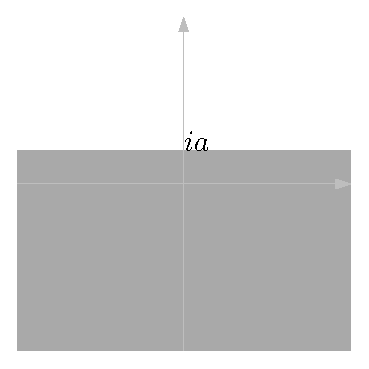
\includegraphics[scale=0.5]{top.eps}
    \end{minipage}
    \begin{minipage}[c]{0.1\textwidth}
        \centering
        \LARGE{$\mapsto$}
    \end{minipage}
    \begin{minipage}[c]{0.45\textwidth}
        \centering
        
\includegraphics[scale=0.5]{parabola.eps}
    \end{minipage}
    \label{fig:24.2}
\end{figure}
Заметим, что данная полуплоскость содержится в $G_{0, \pi}$~--- области
однолистности, значит, функция будет однолистна. Зная, что граница переходит в
границу, отыщем $w(x+ia)$.
\begin{align*}
  & w(x+ia) = (x+ia)^2 = x^2 - a^2 + 2ixa
\end{align*}
\begin{align*}
  & \begin{cases}
      u = x^2 - a^2 \\
      v = 2xa
  \end{cases} \Rightarrow u  = \left( \frac{v}{2a} \right)^2 - a^2
\end{align*}
Поскольку $0$ не лежит в полуплоскости, искомая область будет внешностью
параболы.
\Example
$w = \left| z \right|^{\frac{1}{2}}\exp \left(\dst \frac{i}{2}\argt z\right)$.
\begin{figure}[h!]
    \begin{minipage}[c]{0.45\textwidth}
        \centering
        
\includegraphics[scale=0.5]{parabola.eps}
    \end{minipage}
    \begin{minipage}[c]{0.1\textwidth}
        \centering
        \LARGE{$\mapsto$}
    \end{minipage}
    \begin{minipage}[c]{0.45\textwidth}
        \centering
        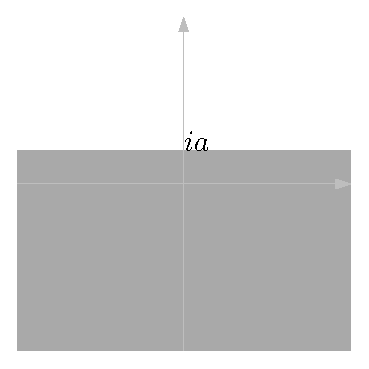
\includegraphics[scale=0.5]{top.eps}
    \end{minipage}
    \label{fig:24.3}
\end{figure}
Обратное к примеру $2$ отображение.
\begin{center}
    \textbf{Экспонента}
\end{center}
Всюду регулярна, но для однолистности необходимо, чтобы не было отличающихся на
$2 i \pi$ элементов (в силу периодичности).
\begin{figure}[h!]
    \centering
    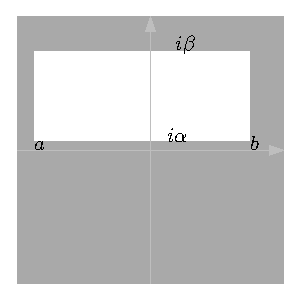
\includegraphics[scale=0.75]{odn_exp.eps}
    \label{fig:24.4}
    \caption{Область однолистности экспоненты}
\end{figure}
\begin{align*}
  & \begin{cases}
      -\infty \leq a \leq b \leq \infty \\
      0 \leq \beta - \alpha < 2 \pi
  \end{cases}
\end{align*}
\Example
\begin{figure}[h!]
    \begin{minipage}[c]{0.45\textwidth}
        \centering
        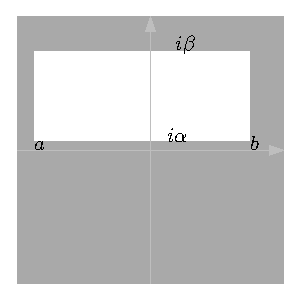
\includegraphics[scale=0.75]{odn_exp.eps}
    \end{minipage}
    \begin{minipage}[c]{0.1\textwidth}
        \centering
        \LARGE{$\mapsto$}
    \end{minipage}
    \begin{minipage}[c]{0.45\textwidth}
        \centering
        
\includegraphics[scale=0.5]{obraz_exp.eps}
    \end{minipage}
    \label{fig:24.5}
\end{figure}
Пусть $z = x+iy_0$, фиксированный $y_0 \in (\alpha,\beta)$. Тогда $\forall x \in
(a,b)$
\begin{align*}
  & f(z) = te^{iy_0}, \ t \in \left( e^{a}, e^{b} \right)
\end{align*}
\Example
~
\\
\begin{figure}[h!]
    \begin{minipage}[c]{0.45\textwidth}
        \centering
        
\includegraphics[scale=0.5]{polupolosa.eps}
    \end{minipage}
    \begin{minipage}[c]{0.1\textwidth}
        \centering
        \LARGE{$\mapsto$}
    \end{minipage}
    \begin{minipage}[c]{0.45\textwidth}
        \centering
        
\includegraphics[scale=0.5]{half_round.eps}
    \end{minipage}
    \label{fig:24.6}
    \caption{Перевод полуполосы в полуокружность.}
\end{figure}
Вертикальная черта переходит в полуокружность, верхняя граница~--- в отрезок
$[-1;0]$, нижняя граница~--- в отрезок $[0;1]$.
\Example
~
\\
\begin{figure}[h!]
    \begin{minipage}[c]{0.45\textwidth}
        \centering
        
\includegraphics[scale=0.5]{d_polupol.eps}
    \end{minipage}
    \begin{minipage}[c]{0.1\textwidth}
        \centering
        \LARGE{$\mapsto$}
    \end{minipage}
    \begin{minipage}[c]{0.45\textwidth}
        \centering
        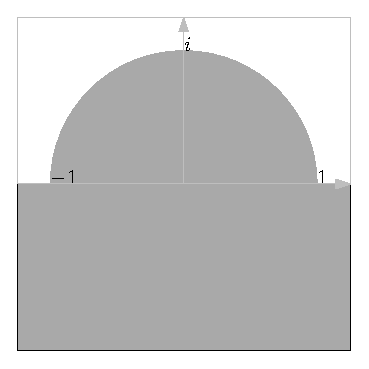
\includegraphics[scale=0.5]{out_rnd.eps}
    \end{minipage}
    \label{fig:24.7}
    \caption{Перевод полуполосы во внешность полуокружности.}
\end{figure}

    \begin{flushright}
    \textit{Лекция 19 (от 09.11)}
\end{flushright}
\begin{center}
    \textbf{Функция Жуковского}
\end{center}
\begin{equation}\label{(24.1)}
    w = \frac{1}{2}\left( z+\frac{1}{z} \right)
\end{equation}
Заметим, что $0$ и $\infty$~--- полюсы $1$ порядка, $\pm 1$~--- нули
производной.
\\
В каждой точке $z \not \in \left\{0, \pm 1,\infty \right\}$ функция конформна. В
точке $0$
\begin{align*}
  & g(z) = \frac{1}{w(z)} = \frac{2z}{z^2+1}
\end{align*}
Эта функция в нуле регулярна и имеет ненулевую производную, а значит, конформна
в нуле. В точке $\infty$
\begin{align*}
  & \varphi(z) = w\left( \frac{1}{z} \right) = \frac{1}{2}\left( \frac{1}{z} + z \right)
\end{align*}
Заметим, что это та же $w$, и в силу конформности в нуле конформна и на
бесконечности. В остальных точках проверим однолистность.
\begin{align*}
  & \frac{1}{2}\left( z_1 + \frac{1}{z_1} \right) - \frac{1}{2}\left( z_1 + \frac{1}{z_1} \right) = 0
\end{align*}
\begin{align*}
  & (z_1-z_2) \left( 1-\frac{1}{z_1z_2} \right)
\end{align*}
\begin{align*}
  & \left[ \begin{matrix}
          z_1=z_2 \\
          z_1z_2 = 1
      \end{matrix} \right.
\end{align*}
Область однолистности $G$: $\pm 1 \not \in G$, $\forall z \in G \ \dst
\frac{1}{z} \not \in G$.
\Example
Функция $w = \dst \frac{1}{z}$ задает две симметрии: относительно единичной
окружности и относительно действительной оси. Соответственно, области
однолистности:
\begin{itemize}
    \item $\left| z \right| < 1$
    \item $\left| z \right| > 1$
    \item $\Img z > 0$
    \item $\Img z < 0$
\end{itemize}
Пусть $z = e^{i \varphi}$, тогда функция Жуковского:
\begin{align*}
  & w = \frac{1}{2}\left( e^{i \varphi} + e^{-i\varphi}\right)
\end{align*}
\begin{equation}\label{(24.2)}
    \begin{cases}
        u = \frac{1}{2}\left( r+\frac{1}{r} \right)\cos \varphi \\
        v = \frac{1}{2}\left( r-\frac{1}{r} \right)\sin \varphi
    \end{cases}
\end{equation}
\Example
~
\begin{itemize}
    \item Пусть задана окружность
    \begin{align*}
      \gamma_r = \left\{ z: \left| z \right| = r, \ r \neq 1\right\}
    \end{align*}
    \begin{align*}
      & \frac{u^2}{a^2} + \frac{v^2}{b^2} = 1, \ a = \frac{1}{2}\left( r + \frac{1}{r} \right), \ b = \frac{1}{2}\left|  r - \frac{1}{r} \right|
    \end{align*}
    \begin{align*}
      & a^2+b^2 = c^2 = 1
    \end{align*}
    Такая окружность переходит в эллипс с фокусами в $\pm 1$, действительной
    полуосью $a$ и мнимой $b$.
    \item Пусть задан луч
    \begin{align*}
      l_\varphi = \left\{ z \mid z = re^{i\varphi}, \ r > 0\right\}, \ \varphi \in [-\pi;\pi) \setminus \left\{ 0, \pm \frac{\pi}{2}, -\pi \right\}
    \end{align*}
    \begin{equation}\label{(24.3)}
        \frac{u^2}{\cos^2 \varphi} - \frac{v^2}{\sin^2\varphi} = 1
    \end{equation}
    Такой луч переходит в гиперболу с фокусами в $\pm 1$.
    \begin{itemize}
        \item $\varphi \in \left( 0; \dst \frac{\pi}{2} \right)$~--- отображение
        в правую ветвь гиперболы, движение по ней вверх.
        \item $\varphi \in \left(\dst \frac{\pi}{2}; \pi \right)$~---
        отображение в левую ветвь гиперболы, движение по ней вверх.
        \item $\varphi \in \left( - \dst \frac{\pi}{2}; 0 \right)$~---
        отображение в правую ветвь гиперболы, движение по ней вниз.
        \item $\varphi \in \left( -\pi; -\dst \frac{\pi}{2} \right)$~---
        отображение в левую ветвь гиперболы, движение по ней вниз.
    \end{itemize}
\end{itemize}
\Example
~
\\
\begin{figure}[h!]
    \begin{minipage}[c]{0.45\textwidth}
        \centering
        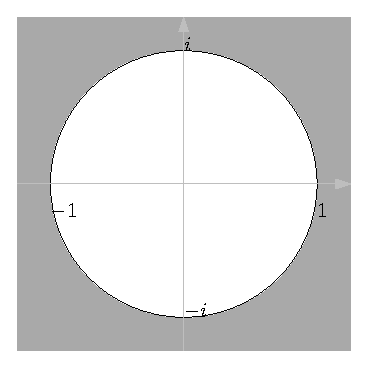
\includegraphics[scale=0.75]{rnd_in.eps}
    \end{minipage}
    \begin{minipage}[c]{0.1\textwidth}
        \centering
        \LARGE{$\mapsto$}
    \end{minipage}
    \begin{minipage}[c]{0.45\textwidth}
        \centering
        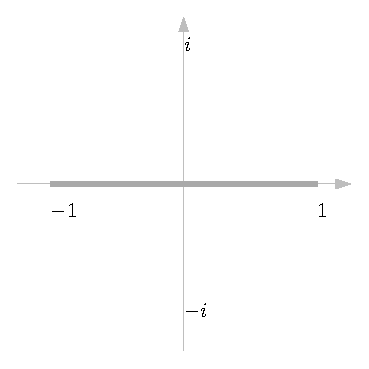
\includegraphics[scale=0.5]{pm1.eps}
    \end{minipage}
    \label{fig:24.10}
    \caption{Перевод единичного круга в $\CC \setminus [-1;1]$}
\end{figure}
\FloatBarrier
\Example
~
\\
\begin{figure}[h!]
    \begin{minipage}[c]{0.45\textwidth}
        \centering
        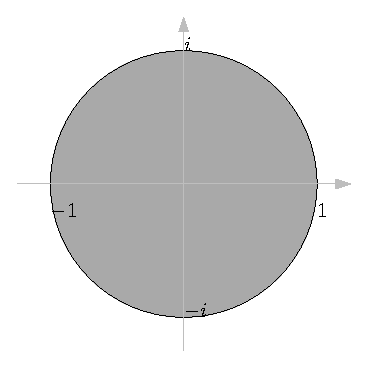
\includegraphics[scale=0.75]{rnd_out.eps}
    \end{minipage}
    \begin{minipage}[c]{0.1\textwidth}
        \centering
        \LARGE{$\mapsto$}
    \end{minipage}
    \begin{minipage}[c]{0.45\textwidth}
        \centering
        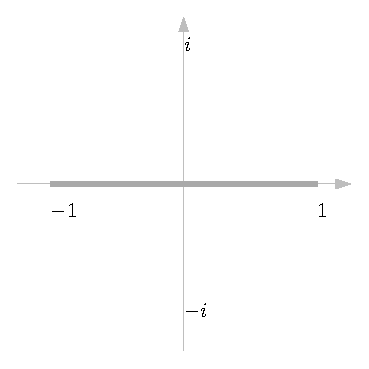
\includegraphics[scale=0.5]{pm1.eps}
    \end{minipage}
    \label{fig:24.11}
    \caption{Перевод внешности единичного круга в $\CC \setminus [-1;1]$}
\end{figure}
\FloatBarrier
\Example
~
\\
\begin{figure}[h!]
    \begin{minipage}[c]{0.45\textwidth}
        \centering
        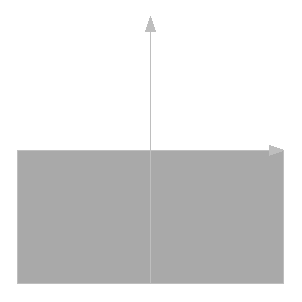
\includegraphics[scale=0.75]{half_plane.eps}
    \end{minipage}
    \begin{minipage}[c]{0.1\textwidth}
        \centering
        \LARGE{$\mapsto$}
    \end{minipage}
    \begin{minipage}[c]{0.45\textwidth}
        \centering
        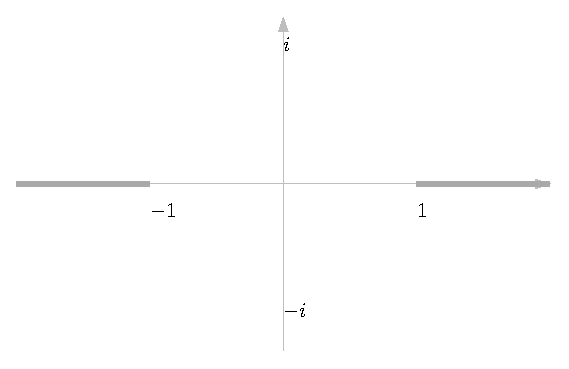
\includegraphics[scale=0.5]{pm1out.eps}
    \end{minipage}
    \label{fig:24.12}
    \caption{Перевод верхней полуплоскости в $\CC \setminus ((-\infty;-1]\cup[1;+\infty)$}
\end{figure}
\FloatBarrier
\Example
~
\\
\begin{figure}[h!]
    \begin{minipage}[c]{0.45\textwidth}
        \centering
        
\includegraphics[scale=0.75]{half_plane_t.eps}
    \end{minipage}
    \begin{minipage}[c]{0.1\textwidth}
        \centering
        \LARGE{$\mapsto$}
    \end{minipage}
    \begin{minipage}[c]{0.45\textwidth}
        \centering
        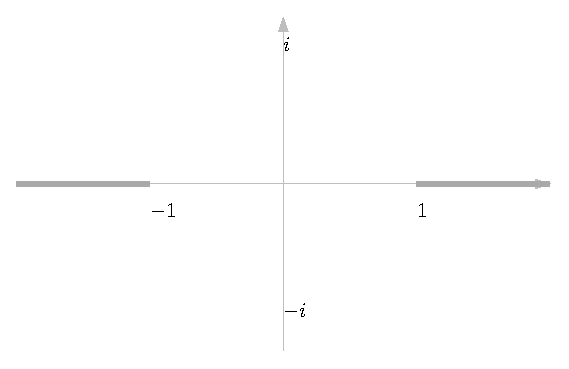
\includegraphics[scale=0.5]{pm1out.eps}
    \end{minipage}
    \label{fig:24.13}
    \caption{Перевод нижней полуплоскости в $\CC \setminus ((-\infty;-1]\cup[1;+\infty)$}
\end{figure}
\FloatBarrier
Отыщем обратную функцию Жуковского.
\begin{align*}
  & w = \frac{1}{2}\left( z+\frac{1}{z} \right) \Rightarrow z^2 - 2wz + 1 = 0
\end{align*}
\begin{align*}
  & z = w \pm g(w), \ g(w) \in \sqrt{w^2-1}
\end{align*}
\Example
Ветвь обратной функции Жуковского, где $g \sim w$ при $w \to \infty$, $z = w -
g(w)$, выполняет следующее преобразование:
\\
\begin{figure}[h!]
    \begin{minipage}[c]{0.45\textwidth}
        \centering
        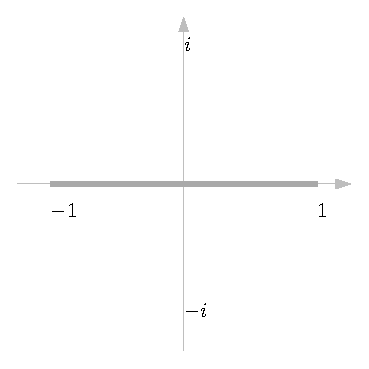
\includegraphics[scale=0.5]{pm1.eps}
    \end{minipage}
    \label{fig:24.14}
    \begin{minipage}[c]{0.1\textwidth}
        \centering
        \LARGE{$\mapsto$}
    \end{minipage}
        \begin{minipage}[c]{0.45\textwidth}
        \centering
        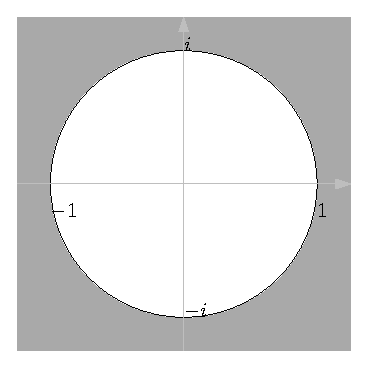
\includegraphics[scale=0.75]{rnd_in.eps}
    \end{minipage}
    \caption{Перевод $\CC \setminus [-1;1]$ в единичный круг}
\end{figure}
\FloatBarrier
\Example
Ветвь обратной функции Жуковского, где $g \sim w$ при $w \to \infty$, $z = w +
g(w)$, выполняет следующее преобразование:
\\
\begin{figure}[h!]
        \begin{minipage}[c]{0.45\textwidth}
        \centering
        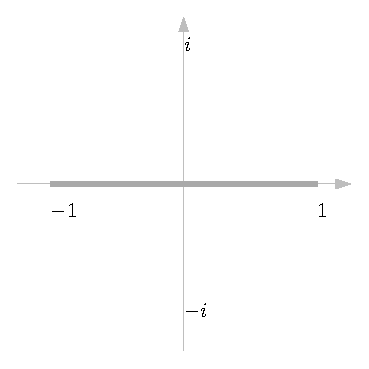
\includegraphics[scale=0.5]{pm1.eps}
    \end{minipage}
    \begin{minipage}[c]{0.1\textwidth}
        \centering
        \LARGE{$\mapsto$}
    \end{minipage}
        \begin{minipage}[c]{0.45\textwidth}
        \centering
        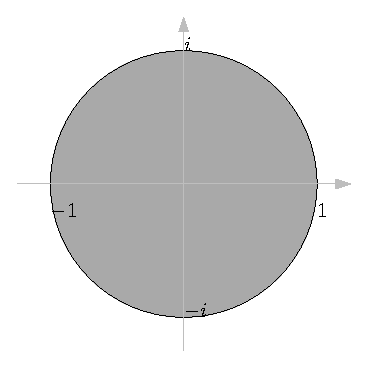
\includegraphics[scale=0.75]{rnd_out.eps}
    \end{minipage}
    \label{fig:24.15}
    \caption{Перевод $\CC \setminus [-1;1]$ во  внешность единичного круга}
\end{figure}
\FloatBarrier
\Example
Ветвь обратной функции Жуковского, где $g(0) = i$, $z = w - g(w)$, выполняет
следующее преобразование:
\\
\begin{figure}[h!]
        \begin{minipage}[c]{0.45\textwidth}
        \centering
        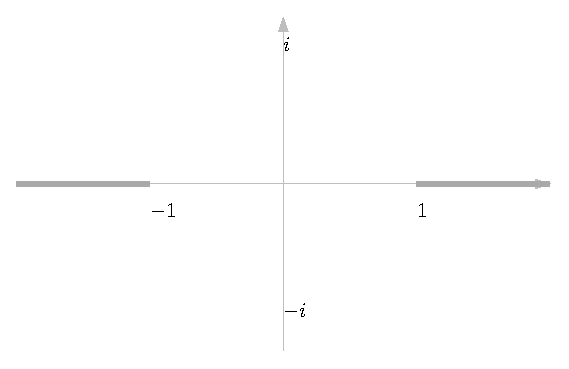
\includegraphics[scale=0.5]{pm1out.eps}
    \end{minipage}
    \begin{minipage}[c]{0.1\textwidth}
        \centering
        \LARGE{$\mapsto$}
    \end{minipage}
    \begin{minipage}[c]{0.45\textwidth}
        \centering
        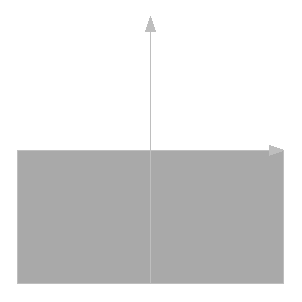
\includegraphics[scale=0.75]{half_plane.eps}
    \end{minipage}
    \label{fig:24.16}
    \caption{Перевод $\CC \setminus (-\infty;-1]\cup[1;+\infty)$ в верхнюю полуплоскость}
\end{figure}
\FloatBarrier
\Example
Ветвь обратной функции Жуковского, где $g(0) = i$, $z = w + g(w)$, выполняет
следующее преобразование:
\\
\begin{figure}[h!]
        \begin{minipage}[c]{0.45\textwidth}
        \centering
        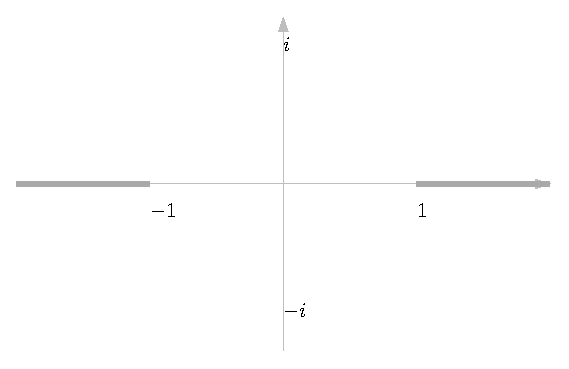
\includegraphics[scale=0.5]{pm1out.eps}
    \end{minipage}
    \begin{minipage}[c]{0.1\textwidth}
        \centering
        \LARGE{$\mapsto$}
    \end{minipage}
    \begin{minipage}[c]{0.45\textwidth}
        \centering
        
\includegraphics[scale=0.75]{half_plane_t.eps}
    \end{minipage}
    \label{fig:24.17}
    \caption{Перевод $\CC \setminus (-\infty;-1]\cup[1;+\infty)$ в нижнюю полуплоскость}
\end{figure}
\FloatBarrier
\begin{center}
    \textbf{Теорема Римана}
\end{center}
$\CC$ нельзя конформно отобразить на единичный круг. Действительно, функция (в
предположении существования) будет ограничена, регулярна (в силу определенности
на всей комплексной плоскости она обязана быть целой), значит, по теореме
Лиувилля это константа, что не является требуемым отображением.
\theorem
Общий вид конформного отображения $B_1(0) \mapsto B_1(0)$:
\begin{equation}\label{(24.4)}
    f(z) = e^{i\beta}\frac{z-a}{1-z\ol{a}}
\end{equation}
\pr
Если $f$ удовлетворяет \eqref{(24.4)}, то $f: B_1(0) \mapsto B_1(0)$ есть ДЛО, а
значит, оно конформно.
\\
Пусть теперь $g: B_1(0) \mapsto B_1(0)$~--- некоторое конформное отображение.
Докажем, что такая функция удовлетворяет \eqref{(24.4)}.
\\
Заметим:
\begin{align*}
  \exists w_0 \in B_1(0): \ g(0) = w_0
\end{align*}
Расмотрим теперь
\begin{align*}
  h(w) = \frac{w-w_0}{1-w\ol{w_0}}, \ h(w_0) = 0, \ h:B_1(0)\mapsto B_1(0)
\end{align*}
Положим
\begin{align*}
  f(z) = h(g(z))
\end{align*}
$f$ регулярна, как суперпозиция регулярных функций, и причем $f(0) = 0$,
$f:B_1(0) \mapsto B_1(0)$. Тогда по лемме Шварца $\forall z \in B_1(0) \ \left|
    f(z) \right|\leq \left| z \right|$.
\\
Тогда $f^{-1}$ таже будет регулярна, $f^{-1}(0) = 0$, $f^{-1}: B_1(0) \mapsto
B_1(0)$. Тогда по лемме Шварца $\forall w \in B_1(0) \ \left| f^{-1}(w)
\right|\leq \left| w \right|$. Подставляя сюда $w = f(z)$, получим $\left| z
\right| \leq \left| f(z) \right|$, т.~е. $\left| z \right| = \left| f(z)
\right|$, и по лемме Шварца выполняется $f(z) = e^{i\alpha}z$.
\\
Тогда $g(z)$~--- ДЛО. Проверим, что $g$ имеет вид \eqref{(24.4)}.
\begin{align*}
& e^{i\alpha}z = h^{-1}(g(z)); \ \exists z_0 \in B_1(0): \ g(z_0) = 0
\end{align*}
\begin{align*}
& e^{i\alpha} = (h^{-1})'(0)(g'(z_0)) = \frac{g'(z_0)}{h'(w_0)}
\end{align*}
\begin{align*}
& \alpha \in \Arg g'(z_0) - \Arg h'(w_0)
\end{align*}
\begin{align*}
& h'(w_0) = \left.\frac{1-w\ol{w_0}+\ol{w_0}(w-w_0)}{(1-w\ol{w_0})^2}\right|_{w=w_0} = 1 - \left| w_0 \right|^2 > 0 \Rightarrow 0 \in \Arg h'(w_0)
\end{align*}
\begin{align*}
& \alpha \in \Arg g'(z_0)
\end{align*}
Рассмотрим теперь 
\begin{align*}
& g_1(z) = e^{i\alpha}\frac{z-z_0}{1-z\ol{z_0}}
\end{align*}
\begin{align*}
&\varphi(z) = g(g_1^{-1}(w)): B_1(0) \mapsto B_1(0)
\end{align*}
\begin{align*}
&\varphi(g_1(z)) = g(w), \ \varphi(0) = 0, \ \Arg \varphi'(0) + \Arg g_1'(0) = \Arg g'(z_0)
\end{align*}
Дифференцируя,
\begin{align*}
& \alpha \in \Arg g_1(0), \ 0 \in \Arg \varphi'(0)
\end{align*}
По лемме Шварца для прямой и обратной функций
\begin{align*}
& \left| \varphi(z) \right| = \left| z \right| \Rightarrow \varphi(z) = z
\end{align*}
(в силу $0 \in \Arg \varphi'(0)$). Но тогда $g_1(z) = g(z)$, и теорема
доказана.
\lemma 
Пусть область $G\subseteq \CC$ такова, что существует конформное $f_0: G \mapsto
B_1(0)$. Тогда любое конформное отображение $G$ на $B_1(0)$ имеет вид
\begin{align*}
  & f(z) = h(f_0(z))
\end{align*}
причем $h$ имеет вид \eqref{(24.4)}.
\pr
Пусть $f_1: G \mapsto B_1(0)$~--- конформное. Рассмотрим 
\begin{align*}
  & \varphi(w) = f_1(f_0^{-1}(w)): B_1(0) \mapsto B_1(0)
\end{align*}
Оно конформно как суперпозиция конформных. По теореме $1$ это ДЛО,
уловлетворяющее \eqref{(24.4)}. Поскольку
\begin{align*}
& f_1(z) = \varphi(f_0(z))
\end{align*}
то лемма доказана.
\theorem (единственности конформных отображений)
Пусть $G$ такова, что существует конформное $f_0:G \mapsto B_1(0)$. Тогда
множество всех конформных отображений $G \mapsto B_1(0)$ зависит от трех
действительных параметров. В частности, такое отображение единственно, если
выполнены условия:
\begin{equation}\label{(24.5)}
f(z_0) = 0, \ \argt f'(z_0) = \alpha \in [0;2\pi), \ z_0 \in G
\end{equation}
\pr
Из леммы $1$ и теоремы $1$ следует утверждение о трех параметрах.
\\
Докажем теперь единственность. Допустим, от противного, существуют $f_1$, $f_2$,
удовлетворяющие \eqref{(24.5)}. Пусть
\begin{align*}
  & \varphi(w) = f_1(f_2^{-1}(w)), \ \varphi(f_2(z)) = f_1(z), \ \varphi(0) = 0
\end{align*}
Значит, $\varphi(z)$ будет ДЛО по лемме $1$. Дифференцируя в $z_0$, имеем
\begin{align*}
    & \argt \varphi'(0) + \Arg f_2'(z_0) = \Arg f_1'(z_0)
\end{align*}
\begin{align*}
  & 0 \in \Arg \varphi'(0) \Rightarrow \varphi(0) = 0, \ z_0 = 0, \ \alpha = 0
\end{align*}
\begin{align*}
  & \varphi(z) = z \Rightarrow f_1(z) = f_2(z)
\end{align*}
\theorem (Римана)
Пусть $G$~--- область в $\CCC$, граница которой содержит более одной точки.
Тогда существует конформное $f: G \mapsto B_1(0)$.
\corollary
Если $G_1 \subseteq \CCC$, $G_2 \subseteq \CCC$, и ганицы каждой содержат более
одной точки, то существует конформное обображение $G_1$ на $G_2$.
\pr
Пусть $f_1: G_1 \mapsto B_1(0)$, $f_2: G_2 \mapsto B_1(0)$, тогда искомое
отображение $\varphi(z) = f_1(f_2^{-1}(z)): G_1 \mapsto G_2$.
\theorem (принцип соответствия границ)
Пусть $G_1, G_2$~--- ограниченные односвязные области в $\CC$ с кусочно гладкими
границами $\Gamma_1, \Gamma_2$. Пусть $f: G_1 \mapsto G_2$~--- конформное; тогда
существует непрерывное продолжение $\tilde{f}$ такое, что оно отображает
$\Gamma_1$ на $\Gamma_2$ с сохранением ориентации.
    \begin{flushright}
    \textit{Лекция 20 (от 10.11)}
\end{flushright}
\section{$\S 25.$ Принцип симметрии.}
\theorem
Пусть заданы области $G$, $G^*$ в верхней полуплоскости с кусочно гладкими
границами $\Gamma$, $\Gamma^*$. Пусть границы содержат конечное чило интервалов
действительной оси $l_1, \dots, l_n$, $l_1^*, \dots, l_n^*$. Пусть $\tilde{G}$,
$\tilde{G^*}$~--- симметричные относительно действительной оси области. Пусть
$f: G \cup \dst \bigcup_{s=1}^n l_s \mapsto G^*\cup \dst \bigcup_{s=1}^n l_s^*$
конформна на $G$ и непрерывна на $G \cup \dst \bigcup_{s=1}^n l_s$ взамно
однозначно отображает $\forall s \in \left\{ 1, \dots, n \right\} \ l_s \mapsto
l_s^*$. Тогда существует (аналитическое) продолжение $f$ на область $G \cup \dst
\bigcup_{s=1}^n l_s \cup \tilde{G}$, конформно отображающее ее на $G^* \cup \dst
\bigcup_{s=1}^n l_s^* \cup \tilde{G^*}$.
\begin{figure}[h!]
    \begin{minipage}[c]{0.5\textwidth}
        \centering
        
\includegraphics[scale=0.75]{1st.eps}
    \end{minipage}
    \begin{minipage}[c]{0.5\textwidth}
        \centering
        
\includegraphics[scale=0.75]{2nd.eps}
    \end{minipage}
    \label{fig:25.1}
\end{figure}
\pr
Зададим функцию $F$ (искомое продолжение).
\begin{equation}\label{(25.1)}
    F(z) = \begin{cases}
        f(z), \ z \in G \cup \bigcup_{s=1}^n l_s \\
        \ol{f(\ol{z})}, \ z \in \tilde{G}
    \end{cases}
\end{equation}
Докажем дифференцируемость. Пусть $z_0 \in \tilde{G}$; тогда
\begin{align*}
  & \exists \varepsilon > 0: \ \forall \Delta z: \ \left| \Delta z \right| < \varepsilon \ z_0+\Delta z \in G
\end{align*}
\begin{align*}
  & \frac{F(z_0+\Delta z) - F(z_0)}{\Delta z} = \frac{\ol{f}(\ol{z_0+\Delta z}) - \ol{f}(\ol{z_0})}{\Delta z} = \ol{\frac{f(\ol{z_0}+\ol{\Delta z}) - f(\ol{z_0})}{\ol{\Delta z}}}
\end{align*}
Тогда
\begin{align*}
  & \ol{z_0} \in G, \ \ol{z_0} +\ol{\Delta z} \in G, \ \exists f'(\ol{z_0}) = \lim_{\Delta z \to 0} \frac{f(\ol{z_0}+\ol{\Delta z}) - f(\ol{z_0})}{\ol{\Delta z}}
\end{align*}
\begin{align*}
  & \exists F'(z_0) = \ol{f'(\ol{z_0})}
\end{align*}
Пусть теперь $x_0 \in l_s$. Докажем, что $F(z)$ непрерывна в $x_0$. Рассмотрим
нижний полукруг окрестности.
\begin{align*}
  & \lim_{z \os{\tilde{G}}{\to} x_0}F(z) = \lim_{\ol{z} \os{G}{\to} x_0}\ol{f(\ol{z})} = \ol{\lim_{\ol{z} \os{G}{\to} x_0}f(\ol{z})} = \ol{f(x_0)} = f(x_0) \in l_s^*
\end{align*}
Аналогично находится предел по верхнему полукругу.
\\
Тогда по теореме о стирании разреза $F(z)$ регулярна в $x_0$ и, значит,
регулярна во всей объединенной области.
\\
Докажем, наконец, однолистность. Область $G$ отображалась однолистно, как и
интервалы; каждая точка $\tilde{G}$ соответствует единственной точке $G$, как и
$\tilde{G^*}$ и $G^*$, а значит, отображение однолистно и на оставшейся части.
\corollary
принцип симметрии можнообобщить на симметрии относительно любой прямой или
окружности.
\pr
Всякую такую кривую можем перевести в действительную ось (область~--- в верхнюю
полуплоскость), применить принцип симметрии и перевести обратно.
\Example
Найти преобразование, переводящее данные области.
\begin{figure}[h!]
    \begin{minipage}[c]{0.45\textwidth}
        \centering
        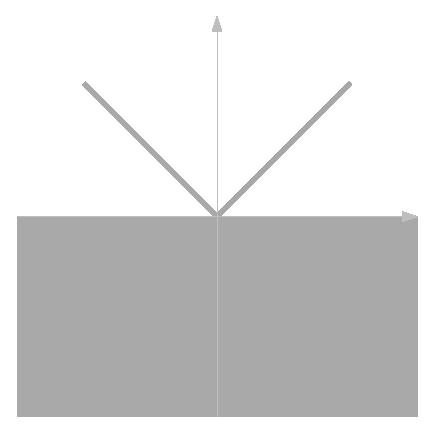
\includegraphics[scale=0.75]{ex24_1.eps}
    \end{minipage}
    \begin{minipage}[c]{0.1\textwidth}
        \centering
        \LARGE{$\mapsto$}
    \end{minipage}
    \begin{minipage}[c]{0.45\textwidth}
        \centering
        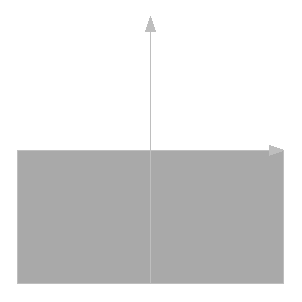
\includegraphics[scale=0.5]{half_plane.eps}
    \end{minipage}
    \label{fig:25.1}
\end{figure}
Воспользовавшись принципом симметрии, рассмотрим лишь правую часть вместе с
мнимой осью. Используя $w_1 = z^4$, получим $\CC \setminus[-4;+\infty)$, причем
функция будет непрерывно продлена на нижний край разреза от нуля и до
бесконечности. Применяя $w_2 = w_1+4$, получим $\CC \setminus[0;+\infty)$, причем
функция будет непрерывно продлена на нижний край разреза от $4$ и до
бесконечности. При помощи $w_3 = \sqrt{\left| w_2 \right|}\exp \left(
\dst \frac{i}{2}\argt w_2\right)$ получаем верхнюю полуплоскость, а $(-\infty;
-2]$ имеет непрерывное продолжение функции на себе. Затем сдвигаем этот разрез:
$w_4 = w_3+2$, и извлекаем корень: $w_5 = \sqrt{\left| w_4 \right|}\exp \left(
    \dst \frac{i}{2}\argt w_4\right)$. По принципу симметрии можем раскрыть все
до полуплоскости.
\begin{center}
    \begin{tabular}{cccc}
      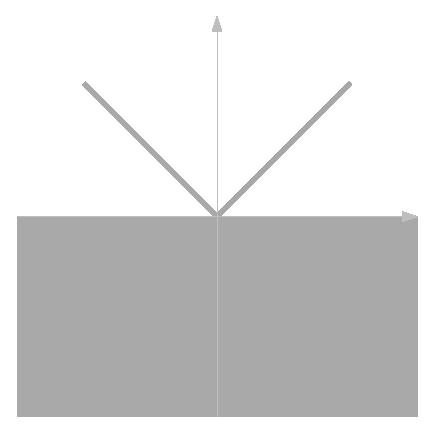
\includegraphics[scale=0.75]{ex24_1.eps} & $\Rightarrow$ & 
\includegraphics[scale=0.75]{2511.eps} & $\mapsto$ \\
      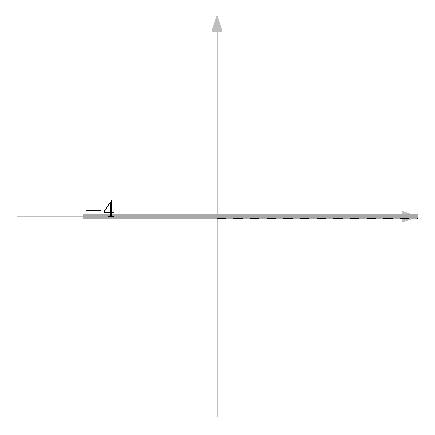
\includegraphics[scale=0.75]{2512.eps} & $\mapsto$ & \includegraphics[scale=0.75]{2513.eps} & $\mapsto$ \\
      \includegraphics[scale=0.75]{2514.eps} & $\mapsto$ & \includegraphics[scale=0.75]{2515.eps} & $\mapsto$ \\
      \includegraphics[scale=0.75]{2516.eps} & $\Rightarrow$ & \includegraphics[scale=1]{half_plane.eps} & \\
    \end{tabular}
\end{center}
\Example
Найти преобразование, переводящее данные области.
\begin{align*}
  & G = \left\{ z = x+iy \mid y^2 < 2p \left( x+\frac{p}{2} \right) \right\}, \ p > 0
\end{align*}
\begin{figure}[h!]
    \begin{minipage}[c]{0.45\textwidth}
        \centering
        \includegraphics[scale=0.75]{2520.eps}
    \end{minipage}
    \begin{minipage}[c]{0.1\textwidth}
        \centering
        \LARGE{$\mapsto$}
    \end{minipage}
    \begin{minipage}[c]{0.45\textwidth}
        \centering
        \includegraphics[scale=0.5]{half_plane.eps}
    \end{minipage}
    \label{fig:25.1}
\end{figure}
Воспользовавшись принципом симметрии, рассмотрим лишь верхнюю часть вместе с
действительной осью. Используя $w_1 = \sqrt{\left| z \right|}\exp \left(\dst
    \frac{i}{2}\argt z\right)$, получаем полуполосу. Растянем эту полуполосу при
помощи $w_2 = \pi\sqrt{\frac{2}{\pi}}$, экспонентой $w_3 = e^{w_2}$ превратим в
верхнюю полуплоскость с вырезанным единичным полукругом. Функцией Жуковского
$w_4 = dst \frac{1}{2}\left( w_3+\dst\frac{1}{w_4} \right)$ переводим в верхнюю
полуплоскость, но она имеет особый участок $[-1;+\infty)$. По принципу симметрии
можем раскрыть это до плоскости с разрезом по $(-\infty;-1]$, и легко, сдвигая
$w_5 = -w_4+1$ и извлекая корень $w_6 = \sqrt{\left| w_5 \right|}\exp \left(\dst
    \frac{i}{2}\argt w_5\right)$, получаем искомое.
\begin{center}
    \begin{tabular}{cccc}
      \includegraphics[scale=0.75]{2520.eps} & $\Rightarrow$ & \includegraphics[scale=0.75]{2521.eps} & $\mapsto$ \\
      \includegraphics[scale=0.75]{2522.eps} & $\mapsto$ & \includegraphics[scale=0.75]{2523.eps} & $\mapsto$ \\
      \includegraphics[scale=0.75]{2524.eps} & $\mapsto$ & \includegraphics[scale=0.75]{2525.eps} & $\Rightarrow$ \\
      \includegraphics[scale=0.75]{2526.eps} & $\mapsto$ & \includegraphics[scale=1]{2527.eps} & $\mapsto$ \\
      \includegraphics[scale=0.5]{half_plane.eps} & & & \\
    \end{tabular}
\end{center}
\section{$\S 26.$ Задача Дирихле на плоскости.}
    \begin{flushright}
    \textit{Лекция 21 (от 16.11)}
\end{flushright}
\theorem
В общей задаче Дирихле при существовании решения в ограниченной области онобудет
единственным. Решение ищем как ограниченную функцию.
\pr
От противного. Допустим, существуют два различных решения $u_1$, $u_2$. Тогда $w
= u_1-u_2 : G \mapsto \RR$, $\Delta w = 0$, $w\Big|_\Gamma = 0$. Тогда по лемме
$1$ $w \equiv 0$.
\Note
Условие ограниченности области является лишь техническим. Условие же
ограниченности функции на области существенно.
\Example
\begin{align*}
  & u(x,y) = \frac{x^2+y^2-2x}{x^2+y^2}
\end{align*}
\begin{align*}
  & G = \left\{ (x,y) \mid x^2+y^2<2x \right\} = \left\{ z: \left| z \right| <1\right\}
\end{align*}
При граничном условии~--- нуле эта функция является решением задачи Дирихле, но
и тождественный нуль также решение. При условии ограниченности эта функция не
подходит.
\begin{center}
    \textbf{Класическая задача Дирихле в круге $B_R(0), \ R > 0$}
\end{center}
\begin{equation}\label{(26.4)}
    \begin{cases}
        \Delta u = 0, \ \left| z \right|< R \\
        u \big|_{\left| z \right| = R} = u_0(z)
    \end{cases}
\end{equation}
причем $u_0(z)$ непрерывна на $\gamma_r$ и решение \eqref{(26.4)} непрерывно на
некотором $B_{R_1}(0), \ R_1 > R$.
\\
Тогда существует регулярная $f: B_{R_1}(0) \mapsto \CC$, что $\Real f(z) =
u(z)$. Тогда по интегральной формуле Коши
\begin{align*}
  & \forall z \in B_R(0) \ f(z) = \frac{1}{2 i \pi} \int_{\gamma_R} \frac{f(\zeta)}{\zeta - z}d\zeta = \frac{1}{2 \pi} \int_{0}^{2\pi} \frac{f(Re^{i\psi})\zeta(\psi)}{\zeta(\psi) - z}d\psi
\end{align*}
Введем теперь симметричную точку $z^* = \dst \frac{R^2}{z}$. Тогда
\begin{align*}
  & \frac{1}{2 i \pi} \int_{\gamma_R} \frac{f(\zeta)}{\zeta - z^*}d\zeta = \frac{1}{2 \pi} \int_{0}^{2\pi} \frac{f(Re^{i\psi})\zeta(\psi)}{\zeta(\psi) - z^*}d\psi = 0
\end{align*}
\begin{align*}
  & f(z) = \frac{1}{2\pi}\int_{0}^{2\pi}f(\zeta(\psi))\left( \frac{\zeta(\psi)}{\zeta(\psi) - z} - \frac{\zeta(\psi)}{\zeta(\psi) - z^*}\right)d\psi = \frac{1}{2\pi}\int_{0}^{2\pi}f(\zeta(\psi))\left( \frac{\zeta(\psi)}{\zeta(\psi) - z} - \right. \\
  & \left. - \frac{\zeta(\psi)\ol{z}}{\zeta(\psi)\ol{\zeta(\psi)} - \zeta(\psi)\ol{z}}\right)d\psi = \frac{1}{2\pi}\int_{0}^{2\pi}f(\zeta(\psi))\left( \frac{\zeta(\psi)\ol{\zeta(\psi)} - z\ol{z}}{\left| \zeta(\psi) - z \right|^2}\right)d\psi = \frac{1}{2\pi}\int_{0}^{2\pi}f(\zeta(\psi))\cdot \\
  & \cdot \left( \frac{\abs{\zeta(\psi)}^2 - \abs{z}^2}{\left| \zeta(\psi) - z \right|^2}\right) d\psi = \frac{1}{2\pi}\int_{0}^{2\pi}f(Re^{i\psi})\left( \frac{R^2 - \abs{z}^2}{\left| Re^{i\psi} - z \right|^2}\right) d\psi
\end{align*}
\begin{equation}\label{(26.5)}
    u(z) = \frac{1}{2\pi}\int_{0}^{2\pi}\tilde{u}_0(\psi)\left( \frac{R^2 - \abs{z}^2}{\left| Re^{i\psi} - z \right|^2}\right) d\psi = \frac{1}{2\pi}\int_{0}^{2\pi}u_0(Re^{i\psi})\left( \frac{R^2 - \abs{z}^2}{\left| Re^{i\psi} - z \right|^2}\right) d\psi
\end{equation}
\eqref{(26.5)} называется \textbf{формулой Пуассона}, интеграл~---
\textbf{интегралом Пуассона}.
\begin{equation}\label{(26.6)}
    K(\zeta,z) = \frac{1}{2\pi} \frac{\abs{\zeta}^2 - \abs{z}^2}{\left| \zeta - z \right|^2}
\end{equation}
\eqref{(26.6)} называется \textbf{ядром (интеграла) Пуассона}.
\begin{equation}\label{(26.7)}
    u(z) = \int_{0}^{2\pi}\tilde{u}_0(\psi)K\left(Re^{i\psi},z\right) d\psi
\end{equation}
\begin{equation}\label{(26.8)}
    K(\zeta,z) = \Real\left( \frac{1}{2\pi} \frac{\zeta+z}{ \zeta - z }\right)
\end{equation}
\begin{align*}
  & f(z) = \frac{1}{2\pi}\int_{0}^{2\pi}\tilde{u}_0(\psi)\frac{\zeta+z}{\zeta-z}d\psi = \frac{1}{2i\pi}\int_{\gamma_R}u_0(\zeta)\frac{\zeta+z}{\zeta-z}\frac{d\zeta}{\zeta}
\end{align*}
\begin{equation}\label{(26.9)}
    u(z) = \Real \frac{1}{2i\pi}\int_{\gamma_R}u_0(\zeta)\frac{\zeta+z}{\zeta-z}\frac{d\zeta}{\zeta}
\end{equation}
\lemma
\begin{align*}
  &\forall z \in B_R(0) \ I(z) = \int_0^{2\pi}K(Re^{i\psi}, z) d\psi = 1
\end{align*}
\pr
\begin{align*}
  & I(z) = \Real I^*(z) = \Real \frac{1}{2\pi}\int_0^{2\pi}\frac{\zeta + z}{\zeta - z} d\psi = \Real \frac{1}{2\pi}\int_{\gamma_R}\frac{\zeta + z}{\zeta - z} \frac{d\zeta}{\zeta} = \Real \left( \us{z}{\res}g(\zeta) + \us{0}{\res}g(\zeta)\right) = \\
  & = \Real(2 - 1) = 1
\end{align*}
\lemma
Пусть $\delta \in \left( 0;\dst \frac{\pi}{2} \right)$, $\zeta_0 \in \gamma_R: \
\zeta_0 = Re^{i\psi_0}, \ \psi_0 \in [0;2\pi)$. Пусть
\begin{align*}
  & \gamma(0, \delta) = \left\{ \zeta \in \gamma_R \mid \zeta = Re^{i\psi}, \ \psi \in (\psi_0+\delta, \psi_0 +2\pi - \delta) \right\}
\end{align*}
Тогда
\begin{align*}
  & \lim_{z \os{B_R(0)}{\to} \zeta_0} \max_{\zeta \in \gamma(0;\delta)}K(\zeta, z) = 0
\end{align*}
\pr
\begin{align*}
  & K(\zeta,z) = \frac{1}{2\pi} \frac{R^2-\abs{z}}{ \abs{\zeta - z }^2}
\end{align*}
$\forall \varepsilon > 0$ рассмотрим $z \in B_\varepsilon(\zeta_0) \cap B_R(0)$;
тогда
\begin{align*}
  & \forall \zeta \in \gamma_R \ \exists \varepsilon > 0: \ \left| \zeta - \zeta_0 \right| = R\left| 1-e^{i(\psi_0-\psi)} \right| > \varepsilon_0, \ \left| z - \zeta_0 \right| < \frac{\varepsilon_0}{2}
\end{align*}
\begin{align*}
  & \forall \zeta \in \gamma_R \ \exists \varepsilon > 0: \ \left| \zeta - z \right| \geq \left| \zeta - \zeta_0 \right| - \left| \zeta_0 - z \right| > \frac{\varepsilon_0}{2}
\end{align*}
\begin{align*}
  & 0 \leq \lim_{z \os{B_R(0)}{\to} \zeta_0} \max_{\zeta \in \gamma(0;\delta)}K(\zeta, z) \leq \lim_{z \os{B_R(0)}{\to} \zeta_0}\frac{2}{\pi\varepsilon_0}\left( R^2-\left| z \right|^2 \right) = 0
\end{align*}
\theorem
Решение общей задачи Дирихле существует в круге $B_r(0)$ и описывается
интегралом Пуассона.
\pr
\begin{equation}\label{(26.10)}
    u(z) = \frac{1}{2\pi}\int_{0}^{2\pi}\tilde{u}_0(\psi)\left( \frac{R^2 - \abs{z}^2}{\left| Re^{i\psi} - z \right|^2}\right) d\psi
\end{equation}
Докажем гармоничность.
\begin{align*}
  & f(z) = \frac{1}{2\pi}\int_{0}^{2\pi}\tilde{u}_0(\psi)\frac{\zeta + z}{\zeta-z}d\psi, \ \zeta = Re^{i\psi}
\end{align*}
Пусть $z \in B_R(0)$, $z+\Delta z\in B_R(0)$. Тогда
\begin{align*}
  & \frac{f(z+\Delta z) - f(z)}{\Delta z} - \frac{1}{\pi}\int_{0}^{2\pi}\tilde{u}_0(\psi)\frac{\zeta}{(\zeta-z)^2}d\psi = \frac{1}{\pi}\int_{0}^{2\pi}\tilde{u}_0(\psi)\left( \frac{z+\Delta z + \zeta}{\zeta - \Delta z - z} + \frac{\zeta + z}{\zeta - z} - \frac{\zeta}{(\zeta-z)^2}\right) d\psi = \frac{1}{\pi}\int_{0}^{2\pi}\tilde{u}_0(\psi)\left( \frac{\zeta}{(\zeta - \Delta z - z)(\zeta - z)} - \frac{\zeta}{(\zeta-z)^2}\right) d\psi = \frac{1}{\pi}\int_{0}^{2\pi}\tilde{u}_0(\psi)\left( \frac{\zeta \Delta z}{(\zeta - \Delta z - z)(\zeta - z)^2}\right) d\psi \us{\Delta z \to 0} 0
\end{align*}
Производная существует, а значит, функция регулярна, а $u$ гармоническая.
\\
Докажем ограниченность. Из определения общей задачи Дирихле на границе за
вычетом конечного числа точек ограничена $u_0(z)$, а поскольку интеграл ядра
равен $1$, то и $u(z)$ ограничена тем же числом.
\\
Докажем непрерывность на границе. Для этого докажем, что
\begin{align*}
  & \lim_{z\os{B_R(0)}{\to} \zeta_0} u(z) = u(\zeta_0)
\end{align*}
Пусть
\begin{align*}
  &\Delta I=  \int_0^{2\pi}\tilde{u}_0(z)K(\zeta(\psi), z)d\psi - u_0(\zeta_0) = \int_0^{2\pi}(\tilde{u}_0-u_0(\zeta_0))K(\zeta(\psi), z)d\psi
\end{align*}
В силу непрерывности $u_0$ в $\zeta_0$
\begin{align*}
  & \forall \varepsilon > 0 \ \exists \delta > 0: \ \left| \psi - \psi_0 \right| < \delta \ \left| u_0(\zeta) - u_0(\zeta_0) \right| <\varepsilon, \ \zeta_0 = Re^{i\varphi_0}
\end{align*}
Положим
\begin{align*}
  & \gamma(1, \delta) = \left\{ \zeta \mid \zeta = Re^{i\psi}, \ \left| \psi - \psi_0 \right| < \delta \right\}, \ \gamma(0, \delta) = \gamma_R\setminus\gamma(1,\delta)
\end{align*}
\begin{align*}
  &\Delta I=  \int_{\psi_0-\delta}^{\psi_0+\delta}(\tilde{u}_0-u_0(\zeta_0))K(\zeta(\psi), z)d\psi + \int_{\psi_0+\delta}^{\psi_0+2\pi-\delta}(\tilde{u}_0-u_0(\zeta_0))K(\zeta(\psi), z)d\psi
\end{align*}
Первый интеграл ограничен сверху $\varepsilon$; для второго же по лемме $2$
$\exists \rho: \ \forall z \in B_\rho(z_0) \max_{\zeta \in
  \gamma(1,\delta)}K(\zeta,z) <\varepsilon$, а значит, модуль интеграла
ограничен сверху $4\pi M \varepsilon$. Значит, можем заметить, что предел
суммарного интеграла будет равен нулю.
\theorem
На ограниченной односвязной области $G$ с кусочно гладкой границей $\Gamma$
существует решение обобщенной задачи Дирихле.
\pr
По теореме Римана существует регулярная $f: G \mapsto B_1(0)$, конформная на
этой области. Тогда $\exists z=g(w): B_1(0) \mapsto G$, и это также конформное
отображение.
\\
То же верно и для замыканий по принципу соответствия границ. Пусть $f(\zeta) =
\alpha$, $g(\alpha) = \zeta$, $\left| \alpha \right|= 1$, $\zeta \in \Gamma$. В
исходной задаче Дирихле $u_0(\zeta)$ непрерына на границе за исключением
конечного числа точек $\tilde{u}(\alpha) = u(g(\alpha))$ обладает тем же
свойством на $\gamma_1$, и по теореме $3$ существует решение $u(w)$ задачи
Дирихле с граничным условием $\tilde{u}(\alpha)$. По формуле Пуассона
\begin{align*}
  & u(w) = \frac{1}{2i\pi}\int_{\gamma_1}\tilde{u}(\alpha)\frac{\alpha + w}{\alpha - w} \frac{d\alpha}{\alpha}
\end{align*}
$u(z) = u(f(z)): G \mapsto \RR$, эта функция гармоническая по теореме $1$, а на
границе $u(\zeta) = u_0(\zeta) = \tilde{u}(\alpha)$. Тогда
\begin{equation}\label{(26.11)}
    u(z) = \Real \frac{1}{2i\pi}\int_{\Gamma}u_0(\zeta)\frac{f(\zeta)+f(z)}{f(\zeta) - f(z)} \frac{f'(\zeta)d\zeta}{f(\zeta)}
\end{equation}
Заметим, что существует дробно-линейное отображение $\Img z > 0 \mapsto B_1(0)$.
Тогда, используя формулу \eqref{(26.11)}, получим теорему:
\theorem
Пусть $u_0(x)$ непрерывна на $\RR$ за исключением, быть может, конечного числа
точек разрыва первого рода, и ограничена. Тогда решение общей задачи Дирихле в
$\Img z > 0$ существует и описывается формулой
\begin{equation}\label{(26.12)}
    u(z) = \frac{1}{\pi}\int_{-\infty}^\infty \frac{y u_0(t)}{(x-t)^2 +y^2} dt, \ z = x+iy
\end{equation}

    \begin{flushright}
    \textit{Лекция 22 (от 17.11)}
\end{flushright}
\section{$\S 27.$ Аналитическое продолжение.}
\Def
Путь задана $f: D \mapsto \CC$, $D \subseteq G \subseteq \CC$, $G$~--- область,
$g: G \mapsto \CC$ регулярна. Если $\forall z \in D \ f(z) = g(z)$, то $g$
называется \textbf{аналитическим продолжением} $f$ на $G$.
\Example
\begin{align*}
  & e^x \to e^z = e^xe^{iy}, \ D = \RR \subseteq \CC \to G = \CC
\end{align*}
\Example
\begin{align*}
  & \sin x \to \sin z = \frac{e^{iz}-e^{-iz}}{2}, \ D = \RR \subseteq \CC \to \CC
\end{align*}
\Def
Пусть $a \in \CC$, $f: B_r(a) \mapsto \CC$, $r>0$~--- регулярная. Тогда $\left(
    B_r(a), f \right)$ называется \textbf{элементом аналитической функции с
  центром в точке $a$}.
\Def
Два элемента $\left( B_r(a), f \right)$ и $\left( B_\rho(b), g \right)$
называются \textbf{эквивалентными}, если $a = b$, $\forall z \in B_{r_0}(a) \
f(z) = g(z)$, $r_0 = \min \left\{ r, \rho \right\}$.
\Def
Пусть $\left( B_r(a), f \right)$~--- элемент аналитической функции, тогда
говорят, что элемент $\left( B_\rho(b), g \right)$ является его
\textbf{непосредственным аналитическим продолжением (НАП)}, если $B_r(a) \cap
B_\rho(b) \neq \varnothing$, $\forall z \in B_r(a) \cap B_\rho(b) \ f(z) =
g(z)$.
\Note
Если определены $B_r(a), B_\rho(b), f$, то по теореме единственности однозначно
определен и $\left( B_\rho(b), g \right)$.
\Def
Пусть $\left( B_r(a), f \right)$~--- элемент. Говорят, что $\left( B_\rho(b), g
\right)$ есть \textbf{аналитическое продолжение элемента $\left( B_r(a), f
  \right)$ вдоль конечной цепочки элементов (кругов)}, если $\exists \left\{
    \left( B_{r_k}(z_k), f_k \right) \right\}_{k=0}^n$ такое, что $\left(
    B_{r_0}(z_0), f_0 \right) \sim \left( B_r(a), f \right)$, $\left(
    B_{r_n}(z_n), f_n \right) \sim \left( B_\rho(b), g \right) $, $\forall k \in
\left\{ 1,\dots, n\right\}$ $\left( B_{r_k}(z_k), f_k \right)$ является
непосредственным аналитическим продолжением $\left( B_{r_{k-1}}(z_{k-1}),
    f_{k-1} \right)$.
\Example
\begin{align*}
  & f_1(z) = \sum_{n=0}^{\infty}z^n
\end{align*}
сходится на $B_1(0)$ и расходится при $\left| z \right| \geq 1$. Пусть $\left(
    B_1(0), f_1 \right)$~--- элемент; тогда
\begin{align*}
  & f_2 = \frac{1}{1-z}
\end{align*}
регулярна в $\CC \setminus \left\{ 1 \right\}$, и для $a \in \CC \setminus [1;
+\infty)$ элемент $\left( B_{\left| a-1 \right|}(a), f_2 \right)$ будет НАП
$\left( B_1(0), f_1 \right)$; для $a_2 \in (1; +\infty)$ элемент $\left(
    B_{\left| a_2-1 \right|}(a_2), f_2 \right)$ не будет НАП $\left( B_1(0), f_1
\right)$, но будет аналитическим продолжением вдоль конечной цепочи кругов.
\Example
Пусть
\begin{align*}
  & f_s(z) = \sqrt{\left| z \right|}\exp\left( \frac{i}{2}\argt_s(z) \right), \ \argt_s(z) \in \left( s-\frac{\pi}{2}, s+\frac{\pi}{2} \right)
\end{align*}
Для элемента $\left( B_1(1), f_0 \right)$ элемент $\left( B_1(i),
    f_{\frac{\pi}{2}} \right)$ будет НАП, а для него, в свою очередь, элемент
$\left( B_1(-1), f_\pi \right)$ будет НАП.
\\
Для элемента $\left( B_1(1), f_0 \right)$ элемент $\left( B_1(-i),
    f_{-\frac{\pi}{2}} \right)$ будет НАП, а для него, в свою очередь, элемент
$\left( B_1(-1), f_{-\pi} \right)$ будет НАП.
\begin{align*}
  & \forall z \in B_1(-1) \ f_\pi(z) = f_{-\pi}(z)
\end{align*}
\section{$\S 28.$ Полные аналитические функции $\Ln z$, $\sqrt[n]{z}$ и римановы
  поверхности.}

    \begin{flushright}
    \textit{Лекция 23 (от 23.11)}
\end{flushright}
\theorem
Пусть $a, b \in \CC \setminus \left\{ 0 \right\}$. Пусть $\left( B_{\left| a
      \right|}(a), h_a \right)$~--- элемент, порожденный $\Ln z$. Тогда для
любой $\gamma_{ab}$, не содержащей нуля, существует аналитическое продолжение в
некоторый элемент $\left( B_{\left| b \right|}(b), h_b \right)$~--- элемент,
порожденный $\Ln z$, причем
\begin{equation}\label{(28.1)}
    h_b(b) = h_a(a) + \int_{\gamma_{ab}}\frac{d\zeta}{\zeta}
\end{equation}
\begin{equation}\label{(28.2)}
    \forall z \in B_{\left| b \right|}(b) \ h_b(z) = h_b(b) + \int_{b}^z\frac{d\zeta}{\zeta}
\end{equation}
$\forall c \in \CC \setminus\left\{ 0 \right\}$, $\forall \left( B_{\left| c
      \right|}(c), h_c\right)$, порожденного $\Ln z$, существует
$\tilde{\gamma}_{ac}$ такая, что этот элемент есть аналитическое продолжение
исходного вдоль этой кривой.
\pr
Заметим, что в силу того, что кривая не содержит нуля, $d = \min \left\{ \left|
        \zeta \right|: \zeta \in \gamma_{ab} \right\} > 0$. Рассмотрим набор
точек $a = z_0, z_1, \dots, z_{K-1}, z_K = b$ на кривой, причем
$l_{\gamma_{z_{k-1}z_k}} \leq \dst \frac{d}{2}$. Зададим для каждой из точек шар
$B_{\left| z_k \right|}z_k$. Заметим, что $\left| z_k- z_{k-1} \right| \leq \dst
\frac{d}{2} < \left| z_{k-1} \right|$. Тогда, как видим, следующая точка лежит в
окрестности предыдущей.
\\
Допустим, доказано существование продолжения на $\gamma_{az_{k-1}}$; докажем
существование $\gamma_{az_k}$. На $B_{\left| z_k \right|}(z_k)$
\begin{equation}\label{(28.3)}
    h_k(z_k) = h_{k-1}(z_{k-1}) + \ln \left| z_k \right| - \ln \left| z_{k-1} \right| + i\Delta_{\gamma_{z_{k-1}z_k}} \argt z = h_{k-1}(z_{k-1}) +\int_{\gamma_{z_{k-1}z_k}} \frac{d\zeta}{\zeta}
\end{equation}
\begin{equation}\label{(28.4)}
    \forall z \in B_{\left| z_k \right|}(z_k) h_k(z) = h_k(z_k) + \int_{z_k}^z \frac{d\zeta}{\zeta}
\end{equation}
Значит, получили искомое продолжение.
\\
Для точки $c$ фиксируем некоторую не содержащую нуля кривую $\gamma_{ac}$. Для
нее существует аналитическое продолжение $\left( B_{\left| c \right|}(c),
    \tilde{h}_c \right)$; и $\exists k \in \ZZ: h_c(z) = \tilde{h}_c(z) + 2 i
\pi k$. Тогда искомая $\tilde{\gamma}_{ac}$ будет равна $\gamma_{ac}$,
объединенной с кругом с центром в нуле и радиусом $c$, обойденным $k$ раз.
\corollary
Полная аналитическая функция $\Ln z$ состоит из элементов $\left( B_{\left| a
      \right|}(a), h_a(z) + 2 i \pi k \right)$, $a \neq 0$, $k \in \ZZ$,
$h_a$~--- регулярная ветвь логарифма.
\begin{align*}
  & \left\{ \sqrt[n]{z} \right\} = \exp \left( \frac{1}{n}\Ln z \right)
\end{align*}
\corollary
Полная аналитическая функция $\left\{ \sqrt[n]{z} \right\}$ состоит из элементов
$\left( B_{\left| a \right|}(a), g_a(z)\exp \left( \frac{i}{n} 2 \pi k
    \right)\right)$, $a \neq 0$, $k \in \left\{ 0, \dots, n-1 \right\}$,
$g_a$~--- регулярная ветвь корня.
\begin{center}
    \textbf{Риманова поверхность $\Ln z$}
\end{center}
\begin{align*}
  & G_0 = \CC \setminus (-\infty; 0]: \ h_0(z) = \ln \left| z \right| + i \argm z, \ \argm z \in (-pi; \pi); \ h_k(z) = h_0(z) + 2 i \pi k, \ k \in \ZZ
\end{align*}
\begin{align*}
  & G_k = \CC \setminus (-\infty; 0]: \\
  & \forall x < 0 \ h_{k-1}(x+i0) = \ln \left| x \right| + i \pi + 2\pi (k-1)i, \  h_{k}(x+i0) = \ln \left| x \right| + i (-\pi) + 2\pi k i
\end{align*}
Значения на верхнем и нижнем краях разреза равны. Можем склеить верхнюю часть
$G_k$ с нижней $G_{k+1}$ для всех $k$. На этой поверхности функция будет
регулярна в любой точке.
\begin{center}
    \textbf{Риманова поверхность $\sqrt{z}$}
\end{center}
\begin{align*}
  & G_0 = \CC \setminus (-\infty; 0]: \ g_0(z) = \sqrt{\left| z \right|} \exp \left( \frac{i}{2} \argm z \right)
\end{align*}
\begin{align*}
  & G_1 = \CC \setminus (-\infty; 0]: \ g_1(z) = -g_0(z)
\end{align*}
\begin{align*}
  & \forall x < 0 \ g_0(x+i0) = i\sqrt{\left| x \right|}, \ g_0(x-i0) = -i\sqrt{\left| x \right|} \\
  & g_1(x+i0) = g_0(x-i0), \ g_1(x-i0) = -g_0(x+i0)
\end{align*}
Значения на верхнем и нижнем краях разреза равны. Можем склеить верхние части с
нижними. На этой поверхности функция будет регулярна в любой точке.
\section{$\S 29.$ Особые точки аналитических функций.}
\Def
Пусть аналитическая функция $F(z)$ такова, что $\exists \gamma_{ab}$: $\forall z
\in \gamma_{ab}\setminus \left\{ b \right\}$ есть аналитическое продолжение
вдоль $\gamma_{az}$, а вдоль $\gamma_{ab}$ его нет. Тогда $b$~--- \textbf{особая
  точка.}
\Def
Пусть $b = \infty$, при замене аргумента $\tilde{F}\left( \
dst \frac{1}{z}\right) = F(z)$ имеет особую точку в нуле, тогда $\infty$~---
\textbf{особая точка} функции $F$.
\Note
Полюса и СОТ регулярной функции~--- особые точки аналитической, а УОТ~--- нет.
\Def
Точка $a$ называется \textbf{точкой ветвления аналитической функции}, если
существует проколотая окрестность, где аналитическая функция определена, но не
однозначно, т.~е. можем в некоторой проколотой окрестности точки $a$ продолжить
функцию, обходя вокруг этой точки, до элемента с той же окрестностью, но другой
функцией.
\Example
$0, \infty$~--- точки ветвления логарифма (никогда не повторяются функции,
логарифмический порядок) и корня (могут повториться, алгебраический порядок).
\theorem (Коши-Адамара)
Пусть степенной ряд
\begin{align*}
  & \sum_{n=0}^\infty c_n(z-a)^n = S(z)
\end{align*}
сходится в круге $B_R(a), \ 0 < a < \infty$. Тогда на границе области (круга)
сходимости существуют особые точки аналитической функции.
\pr
От противного. Пусть $\gamma_R = \left\{ \zeta: \left| \zeta - a \right| = R
\right\}$,
\begin{align*}
  &\forall \zeta \in \gamma_R \ \exists \left( B_{r_\zeta}, f_\zeta \right), \ r_\zeta > 0
\end{align*}
аналитическое продолжение $\left( B_R(a), S(z) \right)$ вдоль радиуса
$\gamma_R$. Всю окружность можно покрыть кругами с центрами в каждой точке, и
существует конечное подпокрытие (лемма Гейне-Бореля), т.~е. конечный набор точек
$\left\{ \zeta_k \right\}_{k=1}^K$ таких, что круги с центрами в них содержат в
себе $\gamma_R$. Получили функцию (аналитическую):
\begin{align*}
  & F(z) = \begin{cases}
      \left( B_R(a), S(z) \right) \\
      \left( B_{r_k}(\zeta_k), f_k \right)
  \end{cases}
\end{align*}
Пусть $G$~--- объединение $B_R(a)$ и всех перечисленных кругов. Докажем
однозначность $F$ на $G$. Рассмотрим $m, n: \ B_{r_n}(\zeta_n)\cap
B_{r_m}(\zeta_m)\neq \varnothing$; тгда в пересечении этих двух кругов с
$B_R(a)$ $f_m(z) = S(z) = f_n(z)$, и по теореме единственности $f_n(z) = f_m(z)$
на пересечении этих двух кругов. Рассмотрим теперь $r = \inf \left\{ \left|
        z-\zeta \right| : z \in B_R(a), \ \zeta \in \CC \setminus G\right\} >
0$; тогда $B_{R+r} \subseteq G$ и $F(z)$ регулярна в этом круге. Ряд
\begin{align*}
  & \sum_{n=0}^\infty \frac{F^{(n)}(z)}{n!}(z-a)^n
\end{align*}
сходится к сумме при $\left| z-a \right|< R$, но тогда этот ряд и в круге
$B_{R+r}$ сходится, противоречие.
\Example
\begin{align*}
  & f(z) = \frac{1}{(z+3)(z^2+2)}
\end{align*}
Радиус сходимости равен $\sqrt{2}$.
\Example
\begin{align*}
  & \frac{1}{1-z} \sum_{n=0}^{\infty} z^n
\end{align*}
Одна особая точка на границе, расходится в них всех.
    \newpage
\section{Additional information}
\end{document}